\documentclass[12pt, a4paper]{book}

\usepackage[T1]{fontenc}
\usepackage{ucs}
\usepackage[utf8x]{inputenc}
\usepackage[english, greek]{babel}

%Fonts
%\usepackage[version=3]{mhchem}
\usepackage{kerkis}

%Paragraph
%\usepackage{indentfirst}
\usepackage{parskip}
\setlength{\parskip}{.5cm}

%Graphics
\usepackage{graphicx}
\usepackage{caption}
\usepackage{subcaption}
%\usepackage{subfloat}
\usepackage{float}
\usepackage{wrapfig}
\usepackage[labelfont=bf]{caption}
\DeclareGraphicsExtensions{.pdf,.png,.jpg}

%Source code
\usepackage{listings} %source code

%Tables
\usepackage{booktabs}
%\usepackage{hhline}

%Page
\usepackage{fullpage}

%Hyper reference
\usepackage[unicode]{hyperref}
\usepackage{xcolor}
\hypersetup{
    colorlinks,
    linkcolor = {blue!100!black},
    citecolor = {blue!100!black},
    urlcolor = {blue!100!black}
}

%Math
\usepackage{amsmath, amsthm, amssymb}
%\usepackage{gfsartemisia-euler}

%URL
\usepackage{url}

%Footnote
\usepackage{threeparttablex}
%\usepackage{footnote}

%Text
\usepackage[normalem]{ulem}
\usepackage{adjustbox}

%Commands

\newcommand{\eng}[1]{\selectlanguage{english}#1\selectlanguage{greek}}
\newcommand{\gre}[1]{\selectlanguage{greek}#1\selectlanguage{english}}

\newcommand{\en}{\selectlanguage{english}}
\newcommand{\gr}{\selectlanguage{greek}}

\newcommand{\norm}[1]{\left\lVert#1\right\rVert}

\begin{document}

%%%%%%%%%%%%%%%%%%%%%%%%%%%%%%%%%%%%%%%%%%%%%%%%%%%%%%%%%%%%%%%%%%%%%%%%%%%%%%%%
\adjustbox{valign=t}{
    \begin{minipage}{0.25\linewidth}
        
\includegraphics[width = 3cm, height=2.8cm]{frontpage/fig/university-patras.jpg}
\end{minipage}}
\hfill
\adjustbox{valign=t}{\begin{minipage}[t]{0.75\linewidth}
    {\Large\textsc{\textbf{Πανεπιστημιο Πατρων}}}\\[5pt]
    {\small\textsc{Τμημα Ηλεκτρολογων Μηχανικων Και Τεχνολογιας Υπολογιστων\\[5pt]
    Τομεας Τηλεπικοινωνιων Και Τεχνολογιας Πληροφοριας\\[5pt]
    Εργαστηριο Απεικονισης Πληροφοριας Kαι Εικονικης Πραγματικοτητας\\}}
\end{minipage}}
\noindent\makebox[\textwidth]{\rule{\textwidth}{0.4pt}}

\vspace{1.5cm}

\begin{center}
    {\Huge\textsc{\textbf{Διπλωματικη Εργασια}}}\\
    {\Large του φοιτητή του Τμήματος Ηλεκτρολόγων Μηχανικών και\\
    Τεχνολογίας Υπολογιστών της Πολυτεχνικής Σχολής του\\
    Πανεπιστημίου Πατρών}\\[2cm]
    {\Large\textsc{\eng{Stanev Dimitar}}}\\[10pt]
    {\Large\textsc{Αριθμός Μητρώου: $7436$}}\\[1.5cm]
    {\Large \uline{Θέμα}}\\[10pt]
    {\Large\textbf{<<Καταγραφή Και Δυναμική Ανάλυση της Κίνησης του Ανθρώπου>>}}\\[2cm]
    {\Large \uline{Επιβλέπων}}\\[10pt]
    {\Large\textsc{Μουστάκας Κωνσταντίνος}}\\[2cm]
    {\Large Αριθμός Διπλωματικής Εργασίας:}\\[2cm]
    {\Large{Πάτρα, Ιουνίου 2014}}
\end{center}

\thispagestyle{empty}
\newpage

%%%%%%%%%%%%%%%%%%%%%%%%%%%%%%%%%%%%%%%%%%%%%%%%%%%%%%%%%%%%%%%%%%%%%%%%%%%%%%%%
\thispagestyle{empty}
\clearpage\mbox{}\clearpage

%%%%%%%%%%%%%%%%%%%%%%%%%%%%%%%%%%%%%%%%%%%%%%%%%%%%%%%%%%%%%%%%%%%%%%%%%%%%%%%%
\begin{center}
    {\HugeΠΙΣΤΟΠΟΙΗΣΗ}\\[1cm]
    Πιστοποιείται ότι η Διπλωματική Εργασία με θέμα\\[0.5cm]
    <<Καταγραφή Και Δυναμική Ανάλυση της Κίνησης του Ανθρώπου>>\\[1cm]
    Του φοιτητή του Τμήματος Ηλεκτρολόγων Μηχανικών και Τεχνολογίας Υπολογιστών\\[0.5cm]
    \eng{STANEV DIMITAR YURIY}\\[10pt]
    Αριθμός Μητρώου: 7436\\[2cm]
    Παρουσιάστηκε δημόσια και εξετάστηκε στο Τμήμα Ηλεκτρολόγων Μηχανικών και Τεχνολογίας Υπολογιστών στις\\
    ..../..../........\\[9cm]
\end{center}

\begin{minipage}[t]{0.5\textwidth}
    \begin{flushleft}
        Ο Επιβλέπων\\
        Μουστάκας Κωνσταντίνος
    \end{flushleft}
\end{minipage}%
\begin{minipage}[t]{0.5\textwidth}
    \begin{flushright}
        Ο Διευθυντής του Τομέα\\
        Φακωτάκης Νίκος
    \end{flushright}
\end{minipage}%

\thispagestyle{empty}
\newpage
\clearpage\mbox{}
\thispagestyle{empty}
\clearpage


%%%%%%%%%%%%%%%%%%%%%%%%%%%%%%%%%%%%%%%%%%%%%%%%%%%%%%%%%%%%%%%%%%%%%%%%%%%%%%%%
\section*{Περίληψη}

Αντικείμενο της παρούσας διπλωματικής εργασίας είναι αρχικά η καταγραφή της κίνησης του ανθρώπου και κατόπιν η δημιουργία ενός αντιπροσωπευτικού μοντέλου ώστε να μπορεί να μελετηθεί η δυναμική του συμπεριφορά. Ως συσκευή καταγραφής χρησιμοποιήθηκε ο αισθητήρας \eng{Kinect} της \eng{Microsoft}. Το μοντέλο του που αναπτύχθηκε αφορά κυρίως τα κάτω άκρα του ανθρώπου και επιπλέον διαθέτει μυοσκελετική δομή. Στα πλαίσια των αναλύσεων χρησιμοποιήθηκαν διάφορες τεχνικές για την εξαγωγή των αποτελεσμάτων όπως είναι η αντίστροφη κινηματική, αντίστροφη δυναμική, υπολογισμός μυϊκών διεγέρσεων και ορθή δυναμική και προτείνουμε μια στρατηγική για την ανάλυση.

Στο πρώτο κεφάλαιο γίνεται μια αναφορά στο πώς οι μεθοδολογίες που αναπτύχθηκαν στα πλαίσια της διπλωματικής εργασίας μπορούν να χρησιμοποιηθούν σε πραγματικές εφαρμογές. Στο δεύτερο κεφάλαιο γίνεται μια ανασκόπηση των χαρακτηριστικών του αισθητήρα, πώς μπορούμε να έχουμε πρόσβαση στα δεδομένα που μας ενδιαφέρουν, τα διάφορα εργαλεία που είναι διαθέσιμα, αλλά και τρόποι μείωσης του θορύβου των μετρήσεων. Στο τρίτο κεφάλαιο γίνεται μια εισαγωγή στις βασικές έννοιες της ρομποτικής δίνοντας μαθηματικούς ορισμούς, που είναι απαραίτητοι για την κατασκευή της διάταξης που θα μελετήσουμε. Στο τέταρτο κεφάλαιο αναφερόμαστε στην μοντελοποίηση των μυών, εστιάζοντας στα μοντέλα \eng{Hill-Type} και εξηγούνται τα στάδια από την στιγμή της παραγωγής νευρικών διεγέρσεων έως την δημιουργία της κίνησης. Στο πέμπτο κεφάλαιο μιλάμε για την ροή της ανάλυσης που ακολουθήθηκε. Τέλος στο έκτο κεφάλαιο παρατείνονται τα αποτελέσματα των πειραμάτων.

%\vspace{6cm}

\paragraph{\textbf{Λέξεις κλειδιά:}}Καταγραφή κίνησης, ορθή δυναμική, αντίστροφη δυναμική, υπολογισμός μυϊκών διεγέρσεων, μυοσκελετικά μοντέλα

\thispagestyle{empty}
\clearpage\mbox{}
\thispagestyle{empty}
\clearpage

%%%%%%%%%%%%%%%%%%%%%%%%%%%%%%%%%%%%%%%%%%%%%%%%%%%%%%%%%%%%%%%%%%%%%%%%%%%%%%%%
\section*{\texorpdfstring{\eng{Abstract}}{}}

\en
The research developed in this thesis first deals with the problem of capturing the human body motion and then concentrates with the creation of multibody model to study its dynamics behavior. The Microsoft's Kinect sensor was used to capture the human motion. As a model we modeled the human lower limb and we attached some muscles on it. For the analysis phase we used inverse kinematics, inverse dynamics, computed muscle control and forward dynamics methods and showed a general pipeline strategy for the analysis.

The first chapter deals with the usage of the methodology developed in this thesis and its applications in real life problems. The second chapter deals with the motion capture sensor, its characteristics, how to access its data, the alternative tools to programm it and a way to deal with noisy measurements. In the third chapter an introduction to some robotics concepts is made, which is necessary for the development of the model. In the forth chapter provides the Hill-Type muscle model and explains how a muscle can generate force for excitation input. In the fifth chapter develops the methods used to analyse the captured data. In the sixth chapter the final results of the analysis are given.
\gr

%\vspace{6cm}

\paragraph{\textbf{\eng{Keywords:}}}\eng{Motion capture, forward dynamics, inverse dynamics, computed muscle control, musculoskeletal models}

\thispagestyle{empty}
\clearpage\mbox{}
\thispagestyle{empty}

%%%%%%%%%%%%%%%%%%%%%%%%%%%%%%%%%%%%%%%%%%%%%%%%%%%%%%%%%%%%%%%%%%%%%%%%%%%%%%%% 
\section*{Ευχαριστίες}

Θα ήθελα να ευχαριστήσω πρώτα από όλα την οικογένεια μου, και ειδικότερα την μητέρα και τον πατέρα μου για τις θυσίες που έκαναν όλο αυτό το καιρό έτσι ώστε να μπορέσω να σπουδάσω. Την κοπέλα μου την Αναστασία για την υποστήριξη και την βοήθεια της κατά την συγγραφή της διπλωματικής μου εργασίας. Τον επιβλέπων καθηγητή μου, κ. Μουστάκα για την ευκαιρία που μου έδωσε να ασχοληθώ με τόσο ενδιαφέρον ερευνητικό πεδίο, αλλά και για την άψογη συνεργασία και βοήθεια που πρόσφερε.

\thispagestyle{empty}
\clearpage

%%%%%%%%%%%%%%%%%%%%%%%%%%%%%%%%%%%%%%%%%%%%%%%%%%%%%%%%%%%%%%%%%%%%%%%%%%%%%%%%
\begin{center}
  \null\vfill
  \large{{\em Αφιερωμένο στην μνήμη του παππού μου}}
  \vspace{2cm}
  \null\vfill
\end{center}

\thispagestyle{empty}

\tableofcontents

\listoffigures

%%%%%%%%%%%%%%%%%%%%%%%%%%%%%%%%%%%%%%%%%%%%%%%%%%%%%%%%%%%%%%%%%%%%%%%%%%%%%%%%
\chapter{Εισαγωγή}

Πολλοί παράγοντες συμβάλουν στην συντεταγμένη κίνηση του σώματος και η γοητεία των επιστημόνων έχει οδηγήσει σε αμέτρητα πειράματα και μελέτες ώστε να μπορούν να την εξηγήσουν. Ως αποτέλεσμα υπάρχει πληθώρα υλικό και αποτελέσματα από μελέτες των χαρακτηριστικών των μυών του σώματος, την γεωμετρική τους συσχέτιση με τα οστά και το αποτέλεσμα της κίνησης των αρθρώσεων. Κατά καιρούς έχουν γίνει κλινικές μελέτες σε ασθένειες όπως είναι η εγκεφαλική παράλυση, το εγκεφαλικό επεισόδιο, η οστεοαρθρίτιδα, η Νόσο του Πάρκινσον ώστε να μελετηθούν οι νευρικές διεγέρσεις που οδηγούν την κίνηση του σώματος τόσο πριν την θεραπεία αλλά και μετά, με σκοπό να εξαχθούν συμπεράσματα για την αντιμετώπιση τους. Δυστυχώς η σύνθεση των δεδομένων από τις κλινικές μελέτες για την κατανόηση της δυσλειτουργίας που οφείλεται στην ασθένεια και την δημιουργία μια επιστημονικής βάσης για την αντιμετώπιση της ανώμαλης κίνησης παραμένει μια σημαντική πρόκληση.

Η χρήση πειραμάτων για την κατανόηση της δυναμικής της κίνησης έχει κάποια μειονεκτήματα. Για παράδειγμα η εκτίμηση των δυνάμεων που παράγονται από τους μύες είναι ακατόρθωτο να μετρηθούν πειραματικά. Επίσης υπάρχει δυσκολία κατανόησης των φαινομένων δράσης-αντίδρασης σε τόσο πολύπλοκα συστήματα μόνο από πειράματα. Ο προσδιορισμός της συνεισφοράς κάθε μυ στην κίνηση δεν είναι προφανές γιατί πολλές φορές η δράση του δεν συνεπάγεται μόνο την επιτάχυνση της άρθρωσης στην οποία δρα \cite{zajac-gordon89} αλλά και σε άλλες αρθρώσεις.

Απαραίτητη προϋπόθεση για την μελέτη πολύπλοκων διατάξεων είναι η ανάπτυξη θεωρητικών μοντέλων που μπορούν να προσεγγίσουν τις ανθρώπινες δραστηριότητες και σε συνδυασμό με τις πειραματικές ενδείξεις να γίνει συστηματική μελέτη. Το σύστημα θα πρέπει να είναι σε θέση να φανερώσει τις εξαρτήσεις μεταξύ του νευρικού, του μυϊκού, του σκελετικού συστήματος και της κίνησης του σώματος. Είναι φανερό ότι τα αποτελέσματα αυτού του είδους αναλύσεων παρέχουν μεγαλύτερη πληροφορία και δίνουν την δυνατότητα στους ερευνητές να εξάγουν κατάλληλη θεραπεία για την ασθένεια.

Τα τελευταία χρόνια και ιδιαίτερα με την ανάπτυξη των υπολογιστών ήμαστε σε θέση να κάνουμε πολύπλοκες προσομοιώσεις σε μικρότερο χρονικό διάστημα (της τάξεων μερικών ωρών) που πριν μια δεκαετία θα χρειαζόταν και μέρες. Ο παράγοντας που βελτιώσε την δραματική μείωση του χρόνου δεν οφείλεται μόνο στην ανάπτυξη των υπολογιστών αλλά και στην εφεύρεση νέων μεθόδων. Η δυναμική προσομοίωση και την ανάπτυξη μυοσκελετικών αλλά και νευρομυοσκελετικά μοντέλων είναι σε θέση να δώσουν λύση σε πολλά προβλήματα που απασχολούν την ιατρική και είναι ευρέως αποδεχτά και έχουν μελετηθεί σε βάθος \cite{thelen-chumanov06, piazza06, pandy01, zajac02}.

Παρόλα αυτά υπάρχουν πολλά προβλήματα και φαινόμενα που δεν έχουν μοντελοποιηθεί ώστε να δώσουν πρόγνωση. Τα μοντέλα που έχουν δημιουργηθεί δεν είναι τόσο ακριβή και υπάρχει περιθώριο βελτιώσεων. Επίσης σε κάποιες αναλύσεις εκτελούνται ακόμα με απαγορευτικούς χρόνους κάνοντας τα ακατάλληλα πολλές φορές. Μεγάλη πρόοδος έχει γίνει στην ανάπτυξη αξιόπιστων μοντέλων για τον μυ, αλλά η μεγάλη διαφοροποίηση που υπάρχει στο ανθρώπινο σώμα καθιστά δύσκολη την χρήση ενός γενικού μοντέλου. Από την άλλη υπάρχει μεγάλο χάσμα στην διασύνδεση του νευρικού συστήματος με το κινητήριο σύστημα και τα μοντέλα που υπάρχουν είναι απλοποιημένα και δεν αναπαριστούν πλήρες τις λειτουργίες του. Συμπερασματικά πρέπει να γίνει πολύ δουλεία τόσο από την μεριά των επιστημόνων που μελετούν την ανθρώπινη φυσιολογία αλλά και των μηχανικών που μοντελοποιούν τα συστήματα ώστε να τα χρησιμοποιήσουν στις προσομοιώσεις.

Είναι αναγκαία η δημιουργία ενιαίων εργαλείων και μοντέλων που θα χρησιμοποιούνται από την επιστημονική κοινότητα στις μελέτες τους. Υπάρχουν πολλά εργαστήρια που έχουν αναπτύξει ενδιαφέρουσες τεχνικές, ωστόσο τα αποτελέσματα τους δεν είναι διαθέσιμα για να χρησιμοποιηθεί από άλλους. Υπάρχουν αρκετά εμπορικά εργαλεία (\eng{Anybody, Adams, Visuals 3D}) που είναι κλειστού κώδικα και δεν δίνουν την δυνατότητα επέκτασης και ευελιξίας. Η ανάγκη αυτή έχει οδηγήσει στην ανάπτυξη του ανοιχτού συστήματος \eng{OpenSim} που υποστηρίζεται από μια μεγάλη κοινότητα με πολλά μοντέλα και αναλυτικές μεθόδους, έχοντας βοηθήσει σημαντικά τους ερευνητές τα τελευταία χρόνια. Δίνοντας την δυνατότητα στους επιστήμονες να μοιράζονται κοινές μεθόδους ανάλυσης, μοντέλα και αποτελέσματα, βοηθάει στην βελτίωση, στην αναπαραγωγή και επιβεβαίωση των αποτελεσμάτων που έχουν εξαχθεί από τρίτους.

%%%%%%%%%%%%%%%%%%%%%%%%%%%%%%%%%%%%%%%%%%%%%%%%%%%%%%%%%%%%%%%%%%%%%%%%%%%%%%%%
\section*{Παραδείγματα}

Ως κλασικό παράδειγμα θα αποδείξουμε ότι τα μυοσκελετικά μοντέλων μπορούν να χρησιμοποιηθούν για να εκτιμηθεί η πορεία θεραπείας ορθοπεδικών εγχειρήσεων. Η βάδιση με λυγισμένα τα γόνατα (\eng{crouch gait}) είναι μια από τις πιο κοινές ανωμαλίες σε άτομα με εγκεφαλική παράλυση. Χαρακτηριστικό αυτής της βάδισης είναι το περπάτημα με λυγισμένα γόνατα και η ανικανότητα να παραχθεί αρκετή δύναμη από τους μύες στο γόνατο ώστε να σηκωθεί η λεκάνη (μια κίνηση που απαιτεί πολύ δύναμη και κόπωση από τους μύες).  Μια αιτία είναι το μικρό μήκος του Ημιτενοντώδη μυ και μερικές φορές η θεραπεία είναι η επιμήκυνση του μυ. Ωστόσο, μπορούν να υπάρχουν και άλλες αιτίες της υπερβολικής κάμψης του γόνατος (π.χ. αδύναμοι καμπτήρες της ποδοκνημικής άρθρωσης), και η επιμήκυνση του Ημιτενοντώδη μπορεί να θέσει σε κίνδυνο την αντοχή των μυών στον αστράγαλο \cite{arnolda06}.

\begin{figure}[H]
    \centering
    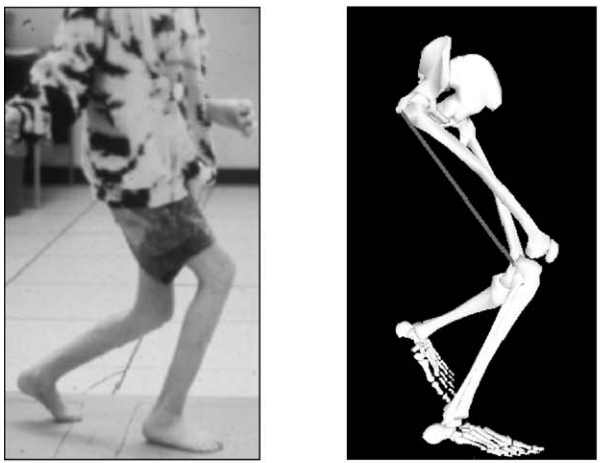
\includegraphics[width=0.8\textwidth]{introduction/fig/crouch-gait.png}
    \caption{Πρόβλημα περπατήματος με λυγισμένα γόνατα\cite{arnolda06}}
    \label{fig:crouch-gait}
\end{figure}

Για αυτό το λόγο μπορούν να γίνουν καταγραφές της βάδισης του ασθενή σε ειδικά εργαστήρια και με κατάλληλο μοντέλο των κάτω άκρων και να μελετηθεί για τον συγκεκριμένο ασθενή αν πρέπει να γίνει η επιμήκυνση του Ημιτενοντώδη. Στα μοντέλα είναι δυνατή η παραμετροποίηση των μυών για το συγκεκριμένο ασθενή ώστε να μελετηθεί με ορθή δυναμική το αποτέλεσμα της εγχείρισης εικονικά. Τέτοιου είδους αναλύσεις θα ήταν ένα χρήσιμο εργαλείο για τους ιατρούς ώστε να τους δώσουν μια εποπτική κατάσταση του ασθενή, να βελτιώσουν την επιτυχία της εγχείρισης αλλά και την δημιουργία μιας θεραπευτικής αγωγής.

Ως δεύτερο παράδειγμα \cite{fregly07} είναι η μελέτη τόπου βαδίσματος ώστε να μειωθεί η καταπόνηση του γονάτου. Σε αυτή την μελέτη οι ασθενείς με προβλήματα οστεοαρθρίτιδα καταπονούν το γόνατο κατά την βάδιση, οπότε οι συγγραφείς προτείνουν μια πολύ απλή παραλλαγή της βάδισης ώστε να μειωθεί η δύναμη που ασκείται στο γόνατο, στρέφοντας ελαφρά το πόδι προστάξω. Κατά το πείραμα οι ασθενείς καταγράφονται από συστήματα παρακολούθησης της κίνησης και επίσης καταγράφεται η αντίδραση εδάφους. Εφαρμόζεται αντίστροφη κινηματική και αντίστροφη δυναμική και σε πραγματικό χρόνο υπάρχει μέτρηση της δύναμης που ασκείται στο γόνατο αλλά και του προσανατολισμού του ποδιού. Στα πλαίσια του πειράματος έχει αναπτυχθεί μια συσκευή που σηματοδοτεί τον ασθενή όταν δεν ακολουθεί τους κανόνες της βάδισης για την μείωση της καταπόντισης. Ως αποτέλεσμα μετά από τέσσερα σεμινάρια οι ασθενείς είχαν συνηθίσει στο νέο τρόπο βάδισης ώστε να μην καταπονούν το γόνατο.

\begin{figure}[H]
    \centering
    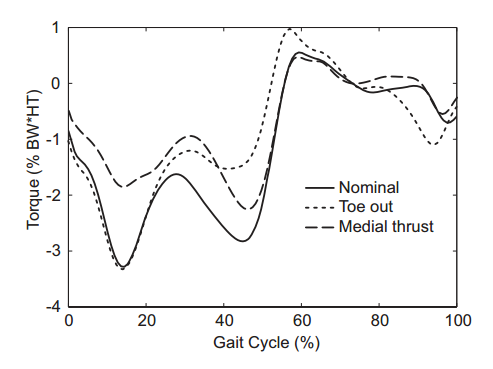
\includegraphics[width=0.8\textwidth]{introduction/fig/knee-load.png}
    \caption{Αποτελέσματα της ροπής της προσαγωγή στο γόνατο\cite{fregly07}}
    \label{fig:knee-load}
\end{figure}

Σαν τρίτο παράδειγμα, θα ήταν ενδιαφέρον να μπορούσαμε να μελετήσουμε την συμπεριφορά των φαρμάκων στις ασθένειες και δραστηριότητες των ανθρώπων. Ως βασικό προαπαιτούμενο απαιτείται η κατανόηση και η μοντελοποίηση της δράσης του φαρμάκου ώστε να μπορεί να προσομοιωθεί. Επίσης απαιτείται η μοντελοποίηση της ασθένειας και το πως αυτή συνδέεται με τις δραστηριότητες του ανθρώπου. Έχουν γίνει μελέτες μοντελοποίησης φαρμάκων όπως είναι η δοπαμίνη για την θεραπεία της Νόσος του Πάρκινσον \cite{haeri05}. Ωστόσο, υπάρχουν δυσκολίες όπως είναι η μοντελοποίηση του βασικά γάγγλια (\eng{basal ganglia}). Παρόλο αυτά μπορούν να εξαχθούν ενδιαφέροντα αποτελέσματα και να εξηγηθούν πράγματα που ίσως δώσουν λύση στην εύρεση μεθόδων θεραπείας δύσκολων ασθενειών.

Συμπερασματικά, οι προσομοιώσεις μπορούν να βοηθήσουν την επιστήμη της ιατρικής και όχι μόνο στο να μελετά την συμπεριφορά μια ασθένειας αλλά και να εξάγει συμπεράσματα θεραπείας και στρατηγικές αγωγής. Οι μέθοδοι προσομοιώσεων χρησιμοποιούνται σε άλλες βιομηχανίες, όπως είναι η βιομηχανία των αυτοκινήτων για την σχεδίαση κινητήρων και έχει μειώσει δραματικά το κόστος κατασκευής τους. Ως εκ τούτου θα πρέπει να χρησιμοποιούνται και στην ιατρική, στην παραγωγή νέων φαρμάκων, την δημιουργία νέων ορθοπεδικών μηχανισμών όπως είναι οι υποστηρικτές σκελετικού συστήματος \cite{stopforth12} και σε πολλούς άλλους κλάδους.


%%%%%%%%%%%%%%%%%%%%%%%%%%%%%%%%%%%%%%%%%%%%%%%%%%%%%%%%%%%%%%%%%%%%%%%%%%%%%%%%
\chapter{Συσκευή Καταγραφής Κίνησης}

Στο παρόν κεφάλαιο θα γίνει μια σύντομη ανασκόπηση των χαρακτηριστικών του αισθητήρα. Θα εξηγήσουμε πως δουλεύει ο αλγόριθμος ανίχνευσης του σκελετού και πώς μπορούμε να έχουμε πρόσβαση στις τροχαίες των αρθρώσεων που είναι απαραίτητες για να γίνει η καταγραφή της κίνησης. Θα αναφέρουμε εναλλακτικά εργαλεία που μπορεί να χρησιμοποιήσει κανείς και θα κάνουμε μια σύγκριση μεταξύ τους. Έπειτα θα περάσουμε στο κομμάτι των μετρήσεων και στο πώς μπορούμε να βελτιώσουμε την ποιότητα τους. Τέλος θα γίνει επίδειξη του συστήματος που υλοποιήθηκε για την καταγραφή της βάδισης.

%%%%%%%%%%%%%%%%%%%%%%%%%%%%%%%%%%%%%%%%%%%%%%%%%%%%%%%%%%%%%%%%%%%%%%%%%%%%%%%%
\section{Αισθητήρας}

Ο αισθητήρας της \eng{Microsoft} που πρωτοεμφανίστηκε το 2009 ήταν μια καινοτομία που αρχικά προοριζόταν για την βιομηχανία των παιχνιδιών, αλλά λόγω των πολύ μεγάλων δυνατοτήτων και σχετικά χαμηλής τιμής σύντομα μπήκε στο στόχαστρο της ανοιχτής κοινότητας η οποία κατάφερε να το \lq χακάρει\rq  και να διαθέσει το πρώτο \eng{API} για πρόσβαση στην συσκευή. Με αποτέλεσμα μετά από λίγο καιρό να βγάλει και η \eng{Microsoft} το αντίστοιχο \eng{API}.

%%%%%%%%%%%%%%%%%%%%%%%%%%%%%%%%%%%%%%%%%%%%%%%%%%%%%%%%%%%%%%%%%%%%%%%%%%%%%%%%
\subsection{Χαρακτηριστικά}

Το \eng{Kinect} βασίζεται σε τεχνολογία λογισμικού η οποία έχει αναπτυχθεί από την \eng{Rare}, θυγατρική της \eng{Microsoft}. Η τεχνολογία της κάμερας αναπτύχθηκε από την ισραηλινή εταιρία \eng{PrimeSense} , η οποία ανέπτυξε ένα σύστημα που μπορεί να ερμηνεύσει συγκεκριμένες χειρονομίες, καθιστώντας δυνατόν τον έλεγχο ηλεκτρονικών συσκευών χωρίς κάποια άλλη συσκευή εισόδου, αλλά μόνο χειρονομίες σώματος. Για να γίνει αυτό δυνατόν χρησιμοποιείτε μια υπέρυθρη κάμερα, ένας προβολέας υπερύθρων και ένα ειδικό μικροτσίπ για να παρακολουθεί την κίνηση των αντικειμένων και τα άτομα σε τρεις διαστάσεις. Αυτό το σύστημα \eng{3D scanner} που ονομάζεται \eng{Light Coding} χρησιμοποιεί μια παραλλαγή εικόνας (χάρτης βάθους) η οποία μπορεί να αναπαρασταθεί σε τρισδιάστατο χώρο. Η συσκευή διαθέτει μία \eng{RGB} (8\-\eng{bits} των τριών καναλιών) κάμερα, αισθητήρα βάθους (11\-\eng{bits} μέχρι 2048 διακριτές στάθμες) και \eng{multi-array} μικρόφωνο και είναι ικανό να παρέχει πλήρη σωματική απεικόνιση \eng{3D}, καταγραφή κίνησης, αναγνώριση προσώπου και δυνατότητες αναγνώρισης φωνής όπως φαίνεται στην εικόνα \ref{fig:kinect-characteristics}.

\begin{figure}[H]
    \centering
    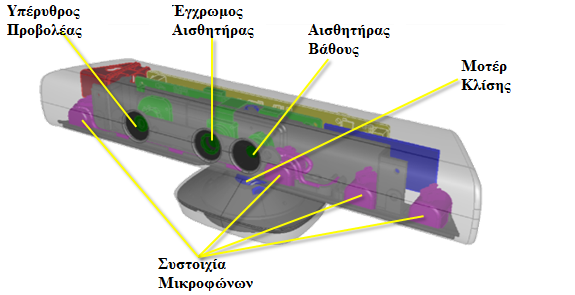
\includegraphics[width=.8\textwidth]{kinect/fig/kinect-characteristics.png}
    \caption{Ο αισθητήρας}
    \label{fig:kinect-characteristics}
\end{figure}

Ο αισθητήρας βάθους αποτελείται από ένα υπέρυθρο προβολέα λέιζερ σε συνδυασμό με ένα μονόχρωμη αισθητήρα \eng{CMOS}, ο οποίος καταγράφει δεδομένα βίντεο σε \eng{3D} κάτω από οποιεσδήποτε συνθήκες φωτισμού. Η τεχνολογία του λογισμικού επιτρέπει την προηγμένη αναγνώριση χειρονομιών, αναγνώριση προσώπου και αναγνώριση φωνής. Σύμφωνα με τις πληροφορίες που παρέχονται στους εμπόρους λιανικής πώλησης, το \eng{Kinect} είναι σε θέση να εντοπίζει ταυτόχρονα έως έξι άτομα. Ο χάρτης βάθους που δημιουργείτε από τον αισθητήρα βάθους, είναι στην ουσία μία εικόνα, η οποία χρησιμοποιώντας διαφορετικές αποχρώσεις χρώματος από λευκό έως μπλε ανάλογα με την απόσταση τον αντικειμένων που 'βλέπει'. Αν σκεφτεί κανείς το μικρό σχετικό κόστος με τις δυνατότητες και την πληροφορία που σου παρέχει το \eng{Kinect} μπορεί κανείς να το συνδυάσει και να δημιουργήσει πολύ ενδιαφέρουσες εφαρμογές \cite{jean13}. Στον πίνακα \ref{tab:sensor-characteristics} συνοψίζονται τα βασικά τεχνικά χαρακτηριστικά λειτουργίας.

\begin{center}
    \begin{tabular}{ll}
        \toprule
        % after \\: \hline or \cline{col1-col2} \cline{col3-col4} ...
        \multicolumn{2}{c}{Χαρακτηριστικά} \\
        \midrule
        Ανάλυση & $1280\times 960, \quad 1024\times 768,$ \\
          & $640\times 480, \quad 320\times 240$ \\
        Υπέρυθρη αόρατη δέσμη & $0.4m$ έως $3.5m$ \\
        Χάρτης βάθους, \eng{RGB} ροή δεδομένων & μέχρι 30 \eng{FPS} \\
        Κάθετης κλίσης & $\pm 27^{o}$ \\
        Κάθετο πεδίο ορατότητας & $43.5^{ο}$ \\
        Οριζόντιο πεδίο ορατότητας & $57^{ο}$ \\
        \bottomrule
    \end{tabular}
    \captionof{table}{Χαρακτηριστικά της συσκευής}
    \label{tab:sensor-characteristics}
\end{center}

\begin{figure}[H]
    \centering
    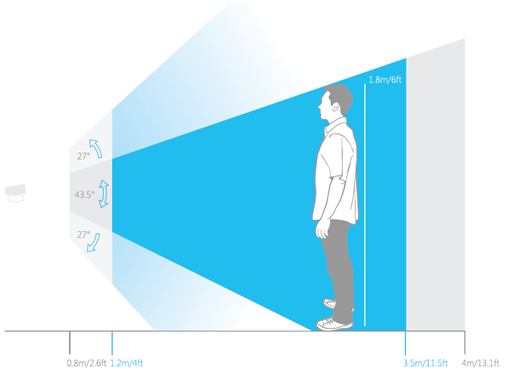
\includegraphics[width=.9\textwidth]{kinect/fig/kinect-operation-mode.png}
    \caption{Περιοχή λειτουργίας}
    \label{fig:kinect-operation-mode}
\end{figure}

%%%%%%%%%%%%%%%%%%%%%%%%%%%%%%%%%%%%%%%%%%%%%%%%%%%%%%%%%%%%%%%%%%%%%%%%%%%%%%%%
\subsection{Αλγόριθμος Ανίχνευση Σκελετού}

Η υλοποίηση ενός αλγορίθμου ανίχνευσης του σκελετού είναι ένα δύσκολο κομμάτι που σχετίζεται με το κλάδο της υπολογιστικής όρασης \cite{mubarak97}, αλλά και άλλων κλάδων. Η ανίχνευση του σκελετού έχει μελετηθεί σε βάθος \cite{thomas00, poppe07} στο παρελθών. Με την δυνατότητα στερεοσκοπικής όρασης, αλλά και τον στόχο να αλληλεπιδρά με τον άνθρωπο η ομάδα έρευνας της \eng{Microsoft} υλοποιείσαι εσωτερικά έναν αλγόριθμο εκτίμησης της στάσης του ανθρώπου και την θέση των αρθρώσεων \cite{shotton11} με κριτήρια, τόσο στην ακρίβεια των αποτελεσμάτων, όσο και στην ταχύτητα για εφαρμογές πραγματικού χρόνο.

\begin{figure}[H]
    \centering
    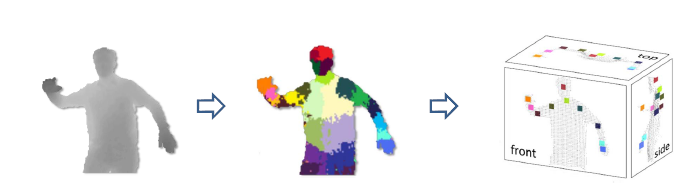
\includegraphics[width=.9\textwidth]{kinect/fig/kinect-skeleton-algorithm.png}
    \caption{Διαδικασία εξαγωγής της θέσης των αρθρώσεων}
    \label{fig:kinect-skeleton-algorithm}
\end{figure}

Ο αλγόριθμος αρχικά εκτιμά τις θέσεις των αρθρώσεων με βάση την εικόνας βάθους μαντεύοντας για κάθε εικονοστοιχείο πόσο πιθανό είναι να βρίσκεται μια άρθρωση στο συγκεκριμένο σημείο δίνοντας ένα επίπεδο εμπιστοσύνης. Έπειτα επιλέγει το σκελετό που είναι πιο πιθανό να δώσει αυτές τις ετικέτες στις αρθρώσεις για τα επίπεδα εμπιστοσύνης. Αλλά πριν μπορέσει να γίνει αυτό, ο αλγόριθμος πρέπει να κάνει ακριβείς εικασίες για τη θέση των αρθρώσεων. Αρχικά, συλλέχθηκαν εικόνες βάθους για τις οποίες ήταν ήδη γνωστή η θέση των αρθρώσεων για να μπορεί να γίνει η εκπαίδευση του αλγορίθμου και συντέθηκα επιπλέον εικόνες με διαφορετικά χαρακτηριστικά σώματος όπως φαίνεται στην εικόνα \ref{fig:kinect-data-synthesis}. Η αναγνώριση βασίζεται στην θεωρία των τυχαίων δέντρων απόφασης (\eng{randomized decision forest}).

\begin{figure}[H]
    \centering
    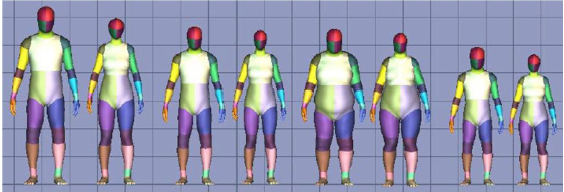
\includegraphics[width=.9\textwidth]{kinect/fig/kinect-data-synthesis.png}
    \caption{Σύνθεσης των εικόνων βάθους για την εκπαίδευση του αλγορίθμου}
    \label{fig:kinect-data-synthesis}
\end{figure}

Το πρόβλημα είναι πολύ δύσκολο και εξαρτάται από πολλούς παράγοντες, όπως είναι το φως, η διαφοροποίηση των ανθρώπων, οι ποικίλες στάσεις, το χρώμα, το δίσημο και από παρεμπόδιση τμημάτων του σώματος που δεν είναι ορατά στον αισθητήρα (\eng{occlusion}). Ο αλγόριθμος επιτυγχάνει πολύ υψηλά ποσοστά ανίχνευσης με μεγάλη ακρίβεια. Είναι ταχύτατος γιατί από την φύση του μπορεί να εκτελεστεί παράλληλα, με αποτέλεσμα η υλοποίηση του να γίνει στο υλικό εσωτερικά και όχι από λογισμικό.

Αυτό που απασχολεί τον χρήστη είναι πως θα μπορέσει να έχει πρόσβαση σε αυτή την πληροφορία. Το πρόβλημα είναι απλό, αφού το \eng{API} διαθέτει συναρτήσεις που σου παρέχουν την δυνατότητα. Ανάλογα με την βιβλιοθήκη που θα χρησιμοποιήσει κανείς για να έχει πρόσβαση στον αισθητήρα πρέπει να μελετήσει τις δυνατότητες που του περεχεί, αλλά και την ευκολία για την ρύθμιση της συσκευής.

%%%%%%%%%%%%%%%%%%%%%%%%%%%%%%%%%%%%%%%%%%%%%%%%%%%%%%%%%%%%%%%%%%%%%%%%%%%%%%%%
\section{Εργαλεία}

Υπάρχουν πολλές εναλλακτικές λύσεις για το πιο εργαλείο μπορεί να χρησιμοποιηθεί για πρόσβαση στα δεδομένα που σου παρέχει το Kinect. Παρακάτω θα αναφερθούν δύο εργαλεία, το προκαθορισμένο \eng{SDK} της \eng{Microsoft} και το εναλλακτικό της \eng{OpenNI}. Και τα δύο είναι εξίσου καλά και χρησιμοποιούνται από πολλούς χρήστες. Τα εργαλεία σου παρέχουν επιπλέον δυνατότητες για πιο προχωρημένες εφαρμογές όπως είναι η αναγνώριση ομιλίας, αναγνώριση έκφρασης προσώπου, τρισδιάστατη ανακατασκευή και άλλα πολλά. Παρακάτω θα αναφερθούν κάποια βασικά χαρακτηριστικά που μας ενδιαφέρουν για το πρόβλημα που θέλουμε να λύσουμε.

%%%%%%%%%%%%%%%%%%%%%%%%%%%%%%%%%%%%%%%%%%%%%%%%%%%%%%%%%%%%%%%%%%%%%%%%%%%%%%%%
\subsection{Προκαθορισμένο Εργαλείο}

Το εργαλείο της \eng{Microsoft} είναι δωρεάν και παρέχει πλούσιο ρεπερτόριο όχι μόνο από συναρτήσεις για πρόσβαση στην συσκευή. Είναι αποκλειστικά για \eng{Windows} και δεν μπορεί να χρησιμοποιηθεί από αλλά λειτουργικά. Οι γλώσσες προγραμματισμού που χρησιμοποιούνται είναι η \eng{C++} και η \eng{C\#}. Υπάρχει δυνατότητα συνεργασία με άλλες βιβλιοθήκες, όπως είναι η \eng{XNA}, \eng{DirectX}.

Όσον αφορά την απόκτηση σκελετικής πληροφορίας υπάρχει μια μεγάλη διαφορά στο ότι το \eng{SDK} της \eng{Microsoft} που σου παρέχει πληροφορία 20 αρθρώσεων. Ένα σημαντικό πλεονέκτημα σε σχέση με άλλα εργαλεία είναι ότι δεν απαιτείται βαθμονόμιση του αισθητήρα. Επίσης μπορεί κανείς να ανιχνεύει μέχρι έξι σκελετούς στην εφαρμογή του. Τέλος, σου παρέχει έτοιμες δομές για φίλτρων για την βελτίωση του αποτελέσματος των θέσεων των αρθρώσεων, που είναι μια απαραίτητη διαδικασία αφού υπάρχει πάντα θόρυβος και προβλήματα εκτίμησης της θέσης. Στην εικόνα \ref{fig:microsoft-sdk-skeleton} φαίνεται ενδεικτικά η δομή του σκελετού που σου προσφέρει το συγκεκριμένο εργαλείο.

\begin{figure}[H]
    \centering
    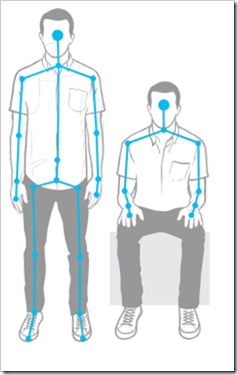
\includegraphics[]{kinect/fig/microsoft-skeleton.png}
    \caption{Σκελετικό σύστημα της \eng{Microsoft}}
    \label{fig:microsoft-sdk-skeleton}
\end{figure}

%%%%%%%%%%%%%%%%%%%%%%%%%%%%%%%%%%%%%%%%%%%%%%%%%%%%%%%%%%%%%%%%%%%%%%%%%%%%%%%%
\subsection{Εναλλακτικά Εργαλεία}

Το εναλλακτικό εργαλείο είναι το OpenNI. Εκτός από το \eng{Kinect} δίνει την δυνατότητα πρόσβασης και σε άλλους αισθητήρες με τον ίδιο τρόπο και έχει μια πολύ ξεκάθαρη αρχιτεκτονική, που διευκολύνει τον προγραμματιστή όπως φαίνεται στην εικόνα \ref{fig:openni-framework}. Όπως και με το \eng{SDK} της \eng{Microsoft} η \eng{OpenNI} σου παρέχει πλούσιο ρεπερτόριο από αλγορίθμους και εφαρμογές. Είναι ανοιχτού κώδικα, υπάρχει υλοποίηση όσο στα \eng{Windows} έτσι και στο \eng{Linux} (\eng{cross platform}). Οι κύριες γλώσσες προγραμματισμού  που υποστηρίζονται από το \eng{OpenNI} είναι η \eng{C++}, η \eng{Java} και \eng{Python}.

\begin{figure}[H]
    \centering
    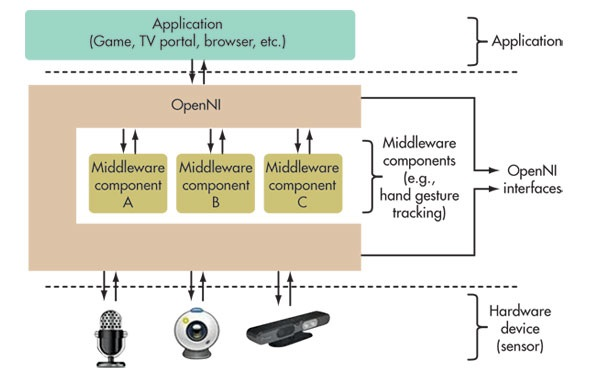
\includegraphics[width=.8\textwidth]{kinect/fig/openni-framework.jpg}
    \caption{Αρχιτεκτονική του \eng{OpenNI}}
    \label{fig:openni-framework}
\end{figure}

\begin{figure}[H]
    \centering
    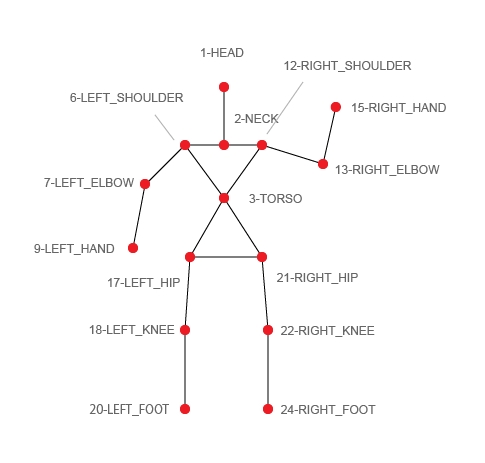
\includegraphics[width=.5\textwidth]{kinect/fig/openni-skeleton.png}
    \caption{Σκελετικό σύστημα του \eng{OpenNI}}
    \label{fig:openni-skeleton}
\end{figure}

Όσον αφορά την εξαγωγή του σκελετού, μειονεκτεί σε σύγκριση με τον αντίστοιχο εργαλείο της \eng{Microsoft}. Αυτό γιατί σου παρέχει 16 αρθρώσεις όπως φαίνεται στην εικόνα \ref{fig:openni-skeleton}, που ίσως δεν είναι αρκετά για την εφαρμογή, ειδάλλως δεν είναι και τόσο κρίσιμη διαφορά. Ένα βασικό μειονέκτημα όμως είναι η απαίτηση βαθμονόμησης της συσκευής. Επίσης κάτι σημαντικό είναι το κομμάτι που αφορά την βελτίωση των μετρήσεων και το \eng{OpenNI} δεν σου παρέχει έτοιμες δομές, κάτι που θα χρειασθεί χρόνο για να υλοποιηθεί. Για τους παραπάνω λόγους προτιμήθηκε το εργαλείο της \eng{Microsoft}. Ενδεικτικά στον πίνακα \ref{tab:openni-microsoft} φαίνονται κάποιες βασικές διαφορές.

\begin{center}
    \begin{tabular}{lcc}
        \toprule
        % after \\: \hline or \cline{col1-col2} \cline{col3-col4} ...
        \multicolumn{1}{c}{Χαρακτηριστικά} & \eng{OpenNI} & \eng{Microsoft SDK} \\
        \midrule
        Πρόσβαση στα δεδομένα βάθους και \eng{RGB} & Ναι & Ναι \\
        Ανίχνευση αρθρώσεων & Ναι & Ναι \\
        Υποστήριξη αναγνώρισης χειρονομιών & Ναι & Όχι \\
        Συναρτήσεις άμεσης αποθήκευσης δεδομένων στο δίσκο & Ναι & Όχι \\
        Βαθμονόμιση & Ναι & Όχι \\
        Υποστήριξη επεξεργασίας ήχου και αναγνώριση ομιλίας & Όχι & Ναι \\
        Ευκολία εγκατάστασης & Όχι & Ναι \\
        Διαθέσιμος αριθμός αρθρώσεων & 16 & 20 \\
        Ποιότητα εγχειριδίων τεκμηρίωση  & Καλή & Μέτρια\\
        \bottomrule
    \end{tabular}
    \captionof{table}{Σύγκριση εναλλακτικών εργαλείων}
    \label{tab:openni-microsoft}
\end{center}

%%%%%%%%%%%%%%%%%%%%%%%%%%%%%%%%%%%%%%%%%%%%%%%%%%%%%%%%%%%%%%%%%%%%%%%%%%%%%%%%
\section{Σύστημα Μετρήσεων}

Οι συλλογή ορθών μετρήσεων είναι ένα σημαντικό βήμα για την εξαγωγή σωστών αποτελεσμάτων στα μετέπειτα στάδια. Η καταγραφή της βάδισης του ανθρώπου είναι η βάση για πολλές αναλύσεις, όπου μπορούν να εξαχθούν χρήσιμα αποτελέσματα. Ενδεικτικά θα ήταν χρήσιμη η μελέτη της δυναμικής συμπεριφοράς του σώματος κατά την διεξαγωγή μιας κίνησης με αποτέλεσμα να μπορεί κανείς να μελετήσει την συμπεριφορά του μυοσκελετικού συστήματος. Πρέπει να δοθεί μεγάλη βαρύτητα στην απόκτηση έγκυρων μετρήσεων, για το λόγο αυτό πρέπει να δημιουργηθούν αλγόριθμοι που να ελαχιστοποιούν τα σφάλματα και να διώχνουν τον θόρυβο. Στην συνέχεια θα εξηγηθούν κάποια ενδεικτικά προβλήματα κατά την διαδικασία της καταγραφής και η αντιμετώπιση τους.

%%%%%%%%%%%%%%%%%%%%%%%%%%%%%%%%%%%%%%%%%%%%%%%%%%%%%%%%%%%%%%%%%%%%%%%%%%%%%%%%
\subsection{Τροχιές των Αρθρώσεων}

Ο προγραμματιστής  μπορεί έχει πρόσβαση στα δεδομένα της συσκευής που αφορούν την συντεταγμένη των αρθρώσεων. Δεδομένου ότι έχει ενεργοποιηθεί εσωτερικά (από τον πρόγραμμα) η ανίχνευση του σκελετού και στο πεδίο ορατότητας της συσκευής ανιχνευθεί αντικείμενο ανθρώπινης μορφής, τότε η συσκευή στέλνει πακέτα με την πληροφορία των θέσεων των αρθρώσεων πίσω στον χρήστη. Το πακέτο περιέχει και επιπλέον πληροφορίες για τις αρθρώσεις όπως είναι ο προσανατολισμός (προϋποθέτει ιεραρχική δομή σκελετού), σκορ εμπιστοσύνης για την μέτρηση (που κυμαίνεται από 0 έως 1) και κάποιες ενδείξεις αν έχει εξαχθεί συμπέρασμα για την θέση της άρθρωσης. Στην ανάλυση ενδιαφερόμαστε για την θέση όσο εξελίσσεται ο χρόνος. Έστω ότι έχουμε $Ν$ αριθμό αρθρώσεων που αποθηκεύονται σε συγκεκριμένες χρονικές στιγμές.

\begin{equation}
    p^{t}_{j} = \{x^{t}_{j}, y^{t}_{j}, z^{t}_{j}\}, \quad t \in (0, t), \quad j \in (0, N)
    \label{equ:trajectories}
\end{equation}

Όπου \eng{p} είναι η Καρτεσιανή θέση την χρονική στιγμή \eng{t} για την άρθρωση \eng{j}. Η αρχή των αξόνων είναι η θέση του \eng{Kinect} και ο άξονας \eng{Z} είναι το βάθος όπως φαίνεται στην εικόνα \ref{fig:kinect-joints}.

\begin{figure}[H]
    \centering
    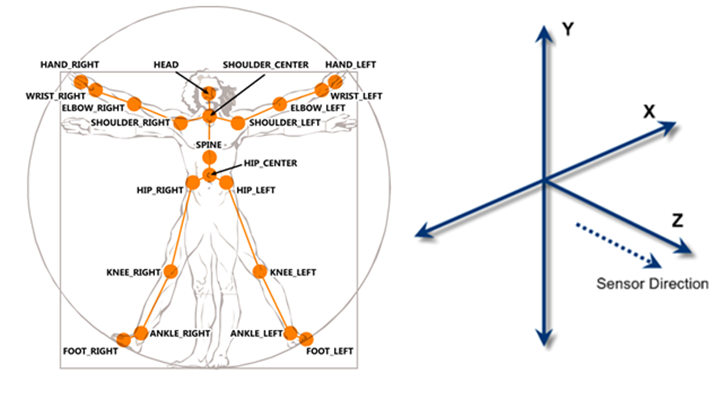
\includegraphics[width=.8\textwidth]{kinect/fig/kinect-joints.png}
    \caption{Σύστημα αρθρώσεων}
    \label{fig:kinect-joints}
\end{figure}

Πρέπει να διευκρινιστεί ότι τα δεδομένα δεν έρχονται περιοδικά σε ντετερμινιστικές χρονικές στιγμές αλλά έχουν μια απόκλιση που οφείλεται κυρίως στο \eng{software} και στις εσωτερικές καθυστερήσεις. Για το λόγο αυτό είναι χρήσιμο να γίνει η μέτρηση της χρονικής στιγμής που έρχονται και αποθηκεύονται τα δεδομένα και να χρησιμοποιηθεί στα μετέπειτα στάδια της ανάλυσης. Μια άλλη παρατήρηση είναι ότι τα δεδομένα είναι στο σύστημα συντεταγμένων με αρχή των αξόνων το \eng{Kinect} και ανάλογα το εργαλείο που θα χρησιμοποιηθεί στα μετέπειτα στάδια της επεξεργασία θα πρέπει να γίνει η κατάλληλη μετατροπή συστήματος συντεταγμένων.

%%%%%%%%%%%%%%%%%%%%%%%%%%%%%%%%%%%%%%%%%%%%%%%%%%%%%%%%%%%%%%%%%%%%%%%%%%%%%%%%
\subsection{Αντιμετώπιση του Θορύβου}

Υπάρχουν πολλά ενοχλητικά προβλήματα που εμφανίζονται στην πράξη και καθιστούν τις μετρήσεις \lq μην κατάλληλες για επεξεργασία\rq . Ο θόρυβος επηρεάζεται από πολλούς παράγοντες, όπως είναι ο φωτισμός στον χώρο που εκτελείται το πείραμα, η στάση του σώματος, η τοποθεσία της συσκευής και πολλά άλλα. Ένα πολύ εμφανές παράδειγμα θορύβου που εμφανίζεται κατά την εκτίμηση της θέσης της άρθρωσης λόγο της μικρής απόκλιση της τιμής από την προηγούμενη μέτρηση με αποτέλεσμα να σου δίνει την αίσθηση ότι το δείγμα τρέμει ενώ στην πραγματικότητα είναι στάσιμο όπως φαίνεται και στην εικόνα \ref{fig:hand2}.

\begin{figure}[h]
    \centering
    \begin{subfigure}[b]{.3\textwidth}
        
\includegraphics[width=\textwidth]{kinect/fig/hand1.png}
        \caption{Ακριβή εκτίμηση}
        \label{fig:hand1}
    \end{subfigure} ~
    \begin{subfigure}[b]{.3\textwidth}
        
\includegraphics[width=\textwidth]{kinect/fig/hand2.png}
        \caption{Εκτίμηση λόγο θορύβου}
        \label{fig:hand2}
    \end{subfigure}
    \caption{Πρόβλημα εκτίμησης θέσης λόγο θορύβου}
\end{figure}

Για την αντιμετώπιση του προβλήματος μπορούν να υλοποιηθούν απλές τεχνικές φιλτραρίσματος και να ελαχιστοποιηθεί ο θόρυβος. Πρέπει κανείς να ξεχωρίσει κάποια κριτήρια που είναι το ποσοστό της εξομάλυνσης των πολύ απότομων κινήσεων, την καθυστέρηση που εισάγεται από την αλλαγή που προκαλεί η φάση του φίλτρου και το αν η εφαρμογή είναι πραγματικού χρόνου (\eng{online}) ή μην πραγματικού χρόνου (\eng{offline}).

Αν επιλεχθεί να αποκοπούν οι ψηλές συχνότητες (απότομες κινήσεις) τότε θα αντιμετωπιστεί το πρόβλημα που αναφέρθηκε πιο πάνω και το αποτέλεσμα θα είναι αυτό της εικόνας \ref{fig:hand1}. Ο θόρυβος αυτής της μορφής στην ξένη βιβλιογραφία αναφέρεται σαν \lq \eng{jitter} \rq . Πρέπει να προσέξουμε όμως γιατί το σύστημα θα αγνοεί πέραν του θορύβου και τις απότομες κινήσεις του δείγματος που ίσως είναι κάτι ανεπιθύμητο. Η σωστή επιλογή αυτών των παραμέτρων είναι κρίσιμη και εξαρτάται από την εφαρμογή που μας ενδιαφέρει και κυρίως από την ταχύτητα του δείγματος.

Όπως φαίνεται στην εικόνα \ref{fig:filter-latency} με κόκκινο είναι η τροχιά, όπου βλέπουμε τις ανεπιθύμητες μεταβολές λόγο θορύβου. Από την άλλη με μπλε χρώμα είναι η τροχιά μετά το φιλτράρισμα, όπου παρατηρούμε ότι έχει εξομαλυνθεί ο θόρυβος, αλλά έχει δημιουργηθεί καθυστέρηση των δειγμάτων. Κάτι που αξίζει να σημειωθεί είναι ότι αν η εφαρμογή δεν απαιτείται να είναι πραγματικού χρόνου, τότε μπορούν να χρησιμοποιηθούν μην αιτιατά φίλτρα, που λαμβάνουν υπόψη στους υπολογισμούς τους μελλοντικές τιμές με αποτέλεσμα να γίνει καλύτερη εκτίμηση της τροχιάς.

\begin{figure}[h]
    \centering
    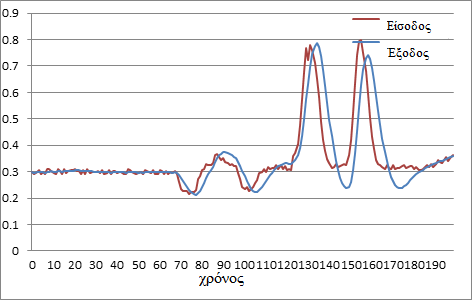
\includegraphics[width=.8\textwidth]{kinect/fig/filter-latency.png}
    \caption{Εξομάλυνση και καθυστέρηση ακολουθίας μετά το φιλτράρισμα}
    \label{fig:filter-latency}
\end{figure}

Για παράδειγμα μια απλή τεχνική για την αφαίρεση του θορύβου λόγο \eng{jitter} βασίζεται στην απλή σχέση αναδρομής \ref{equ:jitter-removal}.

\begin{equation}
    \hat{p}_{n} =
    \begin{cases}
        p_{n}, & \text{Αν } \|p_{n} - \hat{p}_{n-1}\| < \text{κατώφλι} \\
        a \cdot p_{n} + (1-a) \cdot \hat{p}_{n-1}, & \text{αλλιώς}
    \end{cases}
    \label{equ:jitter-removal}
\end{equation}

Στην παρούσα εργασία χρησιμοποιείται μια παραλλαγή του φίλτρου \cite{filter12} \lq \eng{Holt Double Exponential Smoothing}\rq , που έχει άμεση εφαρμογή στα οικονομικά. Τα φίλτρα αυτά στηρίζονται στην παρακάτω αναδρομική σχέση \ref{equ:double-exponential} και οι παράμετροι που επηρεάζουν το αποτέλεσμα δίνονται στο πίνακα \ref{tab:filter-parameters}.

\begin{equation}
    \begin{aligned}
        b_{n} = \gamma \cdot (\hat{p}_{n} - \hat{p}_{n-1}) + (1 - \gamma) \cdot b_{n-1}\\[10pt]
        \hat{p}_{n} = \alpha \cdot p_{n} + (1 - a) \cdot (\hat{p}_{n-1} + b_{n-1})
    \end{aligned}
    \label{equ:double-exponential}
\end{equation}

\vspace{10pt}

\begin{center}
    \begin{threeparttable}
        \begin{tabular}{lccc}
            \toprule
            % after \\: \hline or \cline{col1-col2} \cline{col3-col4} ...
            Παράμετροι & Κανονικό\tnote{α} & Μέτριο\tnote{β} & Δυνατό\tnote{γ} \\
            \midrule
            \eng{Smoothing} & 0.5 & 0.5 & 0.7 \\
            \eng{Correction} & 0.5 & 0.1 & 0.3 \\
            \eng{Prediction} & 0.5 & 0.5 & 1.0 \\
            \eng{JitterRadius} & 0.05 & 0.1 & 1.0 \\
            \eng{MaxDeviationRadius} & 0.04 & 0.1 & 1.0 \\
            \bottomrule
        \end{tabular}
        \begin{tablenotes}
            \item[α] Φιλτράρει ελαφρώς το \eng{jitter}. Καλό για εφαρμογές αναγνώρισης σε παιχνίδια, όπου υπάρχουν απότομες κινήσεις.
            \item[β] Μειώνει αρκετά το \eng{jitter}. Είναι καλό για εφαρμογές όπου απαιτείται ομαλή κίνηση.
            \item[γ] Μειώνει πολύ το \eng{jitter}. Αφορά εφαρμογές που δεν ενδιαφερόμαστε για την καθυστέρηση της κίνησης.
        \end{tablenotes}
    \end{threeparttable}
    \captionof{table}{Ενδεικτικές παράμετρος του φίλτρου}
    \label{tab:filter-parameters}
\end{center}

%\begin{itemize}
%	\item \eng{Smoothing} παράμετρος εξομάλυνσης
%	\item \eng{Correction} μικρές τιμές τείνουν να μοιάζουν με τα δεδομένα που έχουμε
%	\item \eng{Prediction} συμβολίζει την εκτίμηση που κάνουμε για μελλοντικές τιμές
%	\item \eng{JitterRadius} η ακτίνα σε μέτρα για την μείωση του \eng{jitter}
%    \item \eng{MaxDeviationRadius} η μέγιστη διασπορά στην ακτίνα την οποία μπορεί να ανεχτεί το φίλτρο
%\end{itemize}

%%%%%%%%%%%%%%%%%%%%%%%%%%%%%%%%%%%%%%%%%%%%%%%%%%%%%%%%%%%%%%%%%%%%%%%%%%%%%%%%
\section{Υλοποίηση}

Το πρόγραμμα καταγραφής που υλοποιήθηκε έχει σαν στόχο την καταγραφή της χρονικής μεταβολής των θέσεων των αρθρώσεων και την βελτίωση των μετρήσεων. Για να ελαχιστοποιηθούν οι καθυστερήσεις και να μην ελαττωθεί ο ρυθμός επεξεργασίας των πακέτων που εισέρχονται από το \eng{Kinect}, έχουν ενεργοποιηθεί μόνο οι δυνατότητες παρακολούθησης του σκελετού και την πρόσληψη έγχρωμου βίντεο για να μπορούμε να αντιλαμβανόμαστε το ορατό πεδίο του αισθητήρα όπως φαίνεται στην εικόνα \ref{fig:motion-capture}.

\begin{figure}[H]
    \centering
    \includegraphics[width=.9\textwidth]{kinect/fig/motion-capture.png}
    \caption{Σύστημα καταγραφής}
    \label{fig:motion-capture}
\end{figure}

Πρέπει να σημειωθεί ότι η υλοποίηση έγινε με χρήση την βιβλιοθήκη \eng{OpenGL}. Υπάρχουν δύο παράθυρα, όπου στο ένα αναπαριστάται η τελευταία ακολουθία θέσεων του σκελετού, ενώ στο άλλο γίνεται αποτύπωση της έγχρωμης εικόνας που λαμβάνουμε ανά τακτικά χρονικά διαστήματα σαν εικόνα υφής με αποτέλεσμα να έχουμε μια ανανέωση του περιεχομένου (δηλαδή βίντεο). Η περιήγηση στο τρισδιάστατο χώρο του αριστερού παραθύρου μπορεί να γίνει με την βοήθεια του ποντικιού και του πληκτρολογίου δίνοντας την δυνατότητα αναπαράστασης του μοντέλου από διαφορετικές οπτικές γωνίες. 

Εσωτερικά αποθηκεύονται οι παρελθοντικές τιμές των θέσεων σε ειδικές δομές μαζί με όλη την πληροφορία που διαθέτει το \eng{Kinect}. Παρέχεται η δυνατότητα αποθήκευσης των δεδομένων σε δυαδική μορφή η οποία είναι εύκολη στην ανάγνωση και δεν απαιτεί υλοποίηση πολύπλοκων συναρτήσεων ανάγνωσης. Επίσης υπάρχουν επιλογές για αποθήκευσης των τροχιών σε μορφή \lq \eng{.dat}\rq  της \eng{Matlab} και σε μορφή \lq \eng{.trc}\rq , που είναι συμβατή με το εργαλείο \eng{OpenSim}.


%%%%%%%%%%%%%%%%%%%%%%%%%%%%%%%%%%%%%%%%%%%%%%%%%%%%%%%%%%%%%%%%%%%%%%%%%%%%%%%%
\chapter{Περιγραφή Στερεών Σωμάτων}

Στο κεφάλαιο αυτό γίνεται μια σύντομη περιγραφή της μαθηματικής διατύπωσης του προβλήματος της κινηματικής και της δυναμικής των στερεών σωμάτων. Αρχικά μελετούνται οι σχετικοί μετασχηματισμοί που είναι το βασικό εργαλείο περιγραφής της θέσης και του προσανατολισμού των σωμάτων. Έπειτα, γίνεται μια σύντομη περιγραφή της κινηματικής και της διάδοσης των ταχυτήτων σε μια αλυσίδα. Τέλος, επεκτείνεται η ανάλυση στο πρόβλημα της δυναμικής και προτείνεται ένας τρόπος επίλυσης του προβλήματος\footnote{Για περισσότερες πληροφορίες σχετικά με την μοντελοποίηση και την τυποποίηση των εξισώσεων ο αναγνώστης μπορεί να καταφύγει στο \cite{craig95}.}.

%%%%%%%%%%%%%%%%%%%%%%%%%%%%%%%%%%%%%%%%%%%%%%%%%%%%%%%%%%%%%%%%%%%%%%%%%%%%%%%%
\section{Μετασχηματισμοί}

Η θέση και ο προσανατολισμός ενός στερεού σώματος στο χώρο αναφορικά με ένα αδρανειακό καρτεσιανό πλαίσιο συντεταγμένων $\{Β\}$ γίνεται με την περιγραφή της θέσης και του προσανατολισμού ενός καρτεσιανού πλαισίου $\{Α\}$, το οποίο στερεώνουμε σε ένα αυθαίρετο σημείο του σώματος, π.χ. στο κέντρο μάζας. Το διάνυσμα θέσης του πλαισίου $\{Β\}$ εκφρασμένο στο αδρανειακό πλαίσιο $\{Α\}$ με $^AP_{BORG}$ και περιγράφει την θέση του στερεού σώματος και ο πίνακας $^AR_B$ περιγράφει τον προσανατολισμό του σε σχέση με το αδρανειακό σύστημα. Το ζεύγος $\{^AP_{BORG}, ^AR_B\}$ περιγράφουν πλήρες την διάταξη του στερεού σε σχέση με το αδρανειακό \ref{fig:transformation}. Έτσι μπορεί κανείς να εκφράσει την σχετική θέση ενός σημείου στο πλαίσιο $\{Β\}$ ως προς το πλαίσιο  $\{Α\}$ ως εξής:

\begin{equation}
    ^AP = ^AT_B \cdot ^BP, \quad
    ^AT_B =
    \begin{bmatrix}
        ^AR_B & ^AP_{BORG}\\
        0 & 1
    \end{bmatrix}
\end{equation}

\begin{figure}[H]
    \centering
    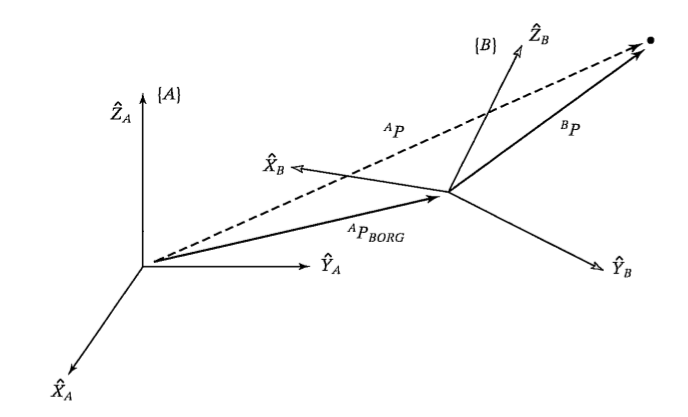
\includegraphics[width=.7\textwidth]{rigidbody/fig/transofrmation.png}
    \caption{Σχετικός μετασχηματισμός}
    \label{fig:transformation}
\end{figure}

Στις περιπτώσεις όπου έχουμε αλυσίδες από πλαίσια που ενώνονται με τους αντίστοιχους σχετικούς μετασχηματισμούς μπορούμε να εκφράσουμε την σχετική θέση ενός πλαισίου πολλαπλασιάζοντας του αντίστοιχους μετασχηματισμούς. Όπως φαίνεται και στην εικόνα \ref{fig:transformation-chain} μπορεί να υπάρχουν εναλλακτικές διαδρομές που περιγράφουν την θέση ενός πλαισίου και οι μετασχηματισμοί που ισχύουν μπορούν να περιγραφούν από τις εξισώσεις \ref{equ:chain}. Σε περίπτωση που υπάρχει κάποιος άγνωστος μετασχηματισμός μπορεί κανείς να λύσει ως προς τον άγνωστο δοσμένου ότι γνωρίζει τους υπόλοιπους.

\begin{figure}[H]
    \centering
    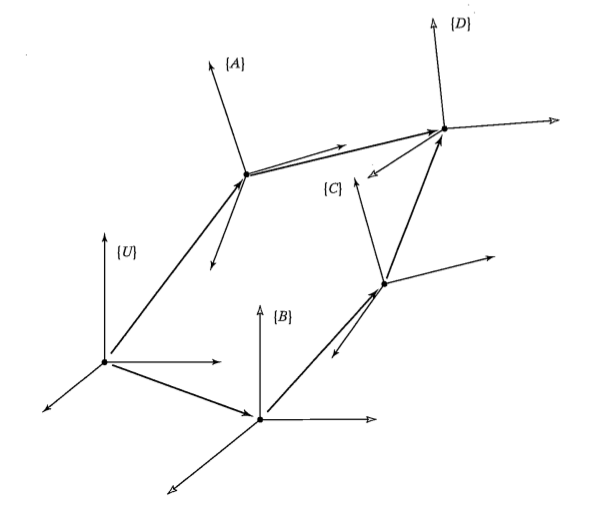
\includegraphics[width=.7\textwidth]{rigidbody/fig/transformation-chain.png}
    \caption{Αλυσίδες μετασχηματισμού}
    \label{fig:transformation-chain}
\end{figure}

\begin{equation}
    \begin{aligned}
        ^UT_D = {}^UT_A \cdot {}^AT_D\\[10pt]
        ^UT_D = {}^UT_B \cdot {}^BT_C \cdot {}^CT_D\\[10pt]
        ^UT_A \cdot ^AT_D = {}^UT_B \cdot {}^BT_C \cdot {}^CT_D
    \end{aligned}
    \label{equ:chain}
\end{equation}

%%%%%%%%%%%%%%%%%%%%%%%%%%%%%%%%%%%%%%%%%%%%%%%%%%%%%%%%%%%%%%%%%%%%%%%%%%%%%%%%
\section{Κινηματική}

Για να κατανοήσουμε το πρόβλημα της κινηματικής, αλλά και της δυναμικής πρέπει να ξεκαθαρίσει τη αλληλεπίδραση των ταχυτήτων σε ένα σύστημα στερεών σωμάτων. Για το λόγο αυτό πριν προχωρήσουμε στην ανάλυση θα γίνει μια μικρή εισαγωγή στο πώς απορρέουν οι εξισώσεις που περιγράφουν την ταχύτητα ενός στερεού με χρήση των σχετικών μετασχηματισμών. Στην συνέχει θα γενικεύσουμε σε συστήματα σωμάτων.

%%%%%%%%%%%%%%%%%%%%%%%%%%%%%%%%%%%%%%%%%%%%%%%%%%%%%%%%%%%%%%%%%%%%%%%%%%%%%%%%
\subsection{Μελέτη της Ταχύτητας}

Έστω ότι θέλουμε να μελετήσουμε την κίνηση ενός σημείου $^BQ$ που ανήκει σε ένα στέρεο σώμα. Στην πιο γενική περίπτωση το σημείο θα έχει μια γραμμική ταχύτητα ως προς κάποιο πλαίσιο $\{Β\}$. Το πλαίσιο $\{Β\}$ θα έχει και αυτό γραμμική και περιστροφική ταχύτητα ως προς κάποιο πλαίσιο παρατήρησης, έστω $\{Α\}$. Θα θέλαμε να εκφράσουμε την ταχύτητα που έχει το σημείο $Q$ ως προς το πλαίσιο παρατήρησης όπως φαίνεται στην εικόνα \ref{fig:velocity}.

\begin{figure}[H]
    \centering
    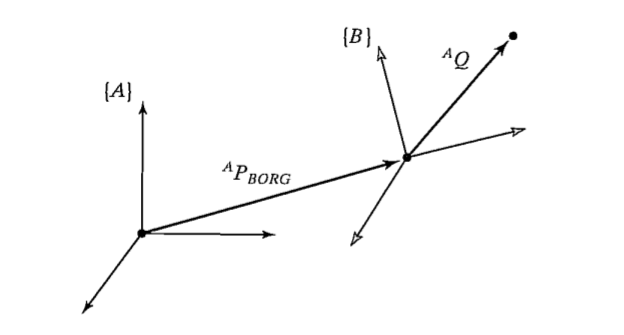
\includegraphics[width=.8\textwidth]{rigidbody/fig/velocity.png}
    \caption{Γενική περίπτωση κίνησης ενός σημείου}
    \label{fig:velocity}
\end{figure}

Έστω ότι η γραμμική ταχύτητα του πλαισίου $\{Β\}$ σε σχέση με το $\{Α\}$ είναι $^AV_{BORG}$ και η γωνιακή ταχύτητα είναι $^A\Omega_{BORG}$. Η γωνιακή ταχύτητα είναι ένα διάνυσμα, όπου η διεύθυνση εκφράζει τον άξονα περιστροφής, ενώ το μέτρο του την γωνία. Επίσης το σημείο $Q$ κινείται με ταχύτητα $^BV_Q$. Η γενική εξίσωση που περιγράφει την κίνηση του σημείου $Q$ δίνεται από την εξίσωση \ref{equ:q-velocity}.

\begin{equation}
    ^AV_Q = {}^AV_{BORG} + {}^AR_B \cdot {}^BV_Q + {}^A\Omega_B \times {}^AR_B
    \cdot {}^BQ
    \label{equ:q-velocity}
\end{equation}

Έστω ότι το σημείο $Q$ είναι αδρανειακό ως προς το πλαίσιο $\{Β\}$. Αν υποθέσουμε ότι το πλαίσιο παρατήρησης $\{Α\}$ συμπίπτει με το πλαίσιο $\{Β\}$, τότε η θέση του σημείο $Q$ ως προς το $\{Α\}$ δίνεται από την εξίσωση \ref{equ:position}.

\begin{equation}
    ^AQ = {}^AR_B \cdot {}^BQ
    \label{equ:position}
\end{equation}

Αν παραγωγίσουμε την σχέση \ref{equ:position} θα πάρουμε την ταχύτητα του σημείου ως προς το $\{Α\}$.

\begin{equation}
    \begin{split}
        ^A\dot{Q} & = {}^A\dot{R}_B \cdot {}^BQ\\
        ^AV_Q & = {}^A\dot{R}_B \cdot {}^AR^{-1}_B \cdot {}^AQ\\
        ^AV_Q & = {}^AS_B \cdot {}^AQ
    \end{split}
    \label{equ:velocity}
\end{equation}

Όπου $^AS_B$ είναι ο αντισυμμετρικός πίνακας και εκφράζεται ως εξής:

\begin{equation}
    ^AS_B  =
    \begin{bmatrix}
        0 & -\Omega_z & \Omega_y\\
        \Omega_z & 0 & -\Omega_x\\
        -\Omega_y & \Omega_x & 0
    \end{bmatrix}
    \label{equ:skew-symmetric}
\end{equation}

%%%%%%%%%%%%%%%%%%%%%%%%%%%%%%%%%%%%%%%%%%%%%%%%%%%%%%%%%%%%%%%%%%%%%%%%%%%%%%%%
\subsection{Μετάδοση της Ταχύτητας}

Ας δούμε το πρόβλημα της μετάδοσης της ταχύτητας από άρθρωση σε άρθρωση όπως φαίνεται στην εικόνα \ref{fig:velocity-transfer}. Θα μελετήσουμε αρχικά την επιρροή της γωνιακής ταχύτητας για την άρθρωση $i+1$ και έπειτα της γραμμικής ταχύτητας. Θα επικεντρωθούμε μόνε σε αρθρώσεις που περιστρέφονται γύρω από τυχαίο άξονα $Ζ$. Η γωνιακή ταχύτητα δίνεται από την σχέση \ref{equ:angular-velocity-propagation}.

\begin{equation}
    ^i\omega_{i+1} = {}^i\omega_i + {}^iR_{i+1} \cdot \dot{q}_{i+1}
    \cdot {}^{i+1}\hat{Z}_{i+1}
    \label{equ:angular-velocity-propagation}
\end{equation}

Αν πολλαπλασιάσουμε την εξίσωση \ref{equ:angular-velocity-propagation} από τις δύο μεριές με $^{i+1}R_i$ μπορούμε να εκφράσουμε το αποτέλεσμα στο πλαίσιο $\{i+1\}$ θα εξάγουμε την εξίσωση \ref{equ:angular-velocity-propagation-final}.

\begin{equation}
    ^{i+1}\omega_{i+1} = {}^{i+1}R_i \cdot {}^i\omega_i + \dot{q}_{i+1}
    \cdot {}^{i+1}\hat{Z}_{i+1}
    \label{equ:angular-velocity-propagation-final}
\end{equation}

Όσον αφορά την γραμμική ταχύτητα η σχέση δίνεται από την εξίσωση \ref{equ:velocity-propagation}.

\begin{equation}
    ^iu_{i+1} = {}^iu_i + {}^i\omega_i \times {}^iP_{i+1}
    \label{equ:velocity-propagation}
\end{equation}

Αν πολλαπλασιάσουμε ξανά την εξίσωση \ref{equ:velocity-propagation} με $^{i+1}R_i$ θα έχουμε την σχέση \ref{equ:velocity-propagation-final}.

\begin{equation}
    ^{i+1}u_{i+1} = {}^{i+1}R_i \cdot (^iu_i + {}^i\omega_i \times
    {}^iP_{i+1})
    \label{equ:velocity-propagation-final}
\end{equation}

\begin{figure}[H]
    \centering
    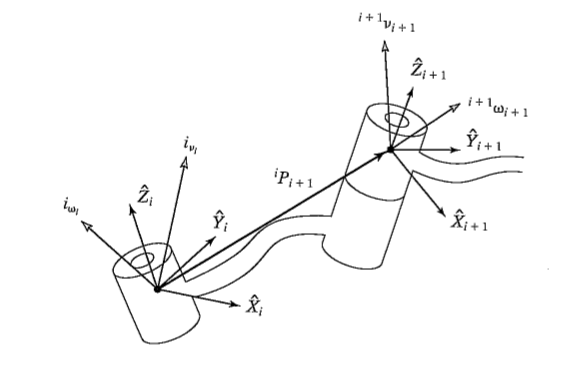
\includegraphics[width=.8\textwidth]{rigidbody/fig/velocity-transfer.png}
    \caption{Μετάδοση της ταχύτητας από άρθρωση σε άρθρωση}
    \label{fig:velocity-transfer}
\end{figure}

%%%%%%%%%%%%%%%%%%%%%%%%%%%%%%%%%%%%%%%%%%%%%%%%%%%%%%%%%%%%%%%%%%%%%%%%%%%%%%%%
\subsection{Αντίστροφη Κινηματική}

Η αντίστροφη κινηματική είναι ένα σημαντικό εργαλείο στα στάδια την διεξαγωγής του πειράματος. Με λίγα λόγια είναι η διαδικασία που μετατρέπει τις θέσεις των αρθρώσεων στο καρτεσιανό τρισδιάστατο χώρο σε γενικευμένες συντεταγμένες του μοντέλου (γωνίες), έτσι ώστε κάθε χρονική στιγμή το μοντέλο να είναι στην ίδια διάταξη με τις μετρήσιμες θέσεις των αντίστοιχων αρθρώσεων. Παρακάτω θα δοθεί η μαθηματική διατύπωση για την λύση του προβλήματος και θα επισημανθούν κάποια λεπτά σημεία που ίσως οδηγήσουν σε λάθος αποτελέσματα.

Δοθέντος ενός συστήματος σωμάτων με $Ν$ βαθμών ελευθερίας με γενικευμένη συντεταγμένη $q^{t}_{j}$ και δοσμένη χρονική ακολουθία από θέσεις για κάθε άρθρωση του μοντέλου $p^{t}_{j}$ με $j \in (1 N)$. Το πρόβλημα της εύρεσης των γενικευμένων συντεταγμένων για κάθε άρθρωση ώστε να ελαχιστοποιηθεί το σφάλμα της απόστασης μεταξύ της παρατήρησης και της στάσης του μοντέλου μπορεί να μοντελοποιηθεί σαν πρόβλημα βελτιστοποίησης \cite{sherman13}. Στόχος είναι η ελαχιστοποίηση του σφάλματος, όπου το σφάλμα είναι η αθροιστική συνάρτηση απόστασης μεταξύ μοντέλου και τις θέσεις των θέσεων. Σαν συνάρτηση απόστασης μπορεί να επιλεγεί η Ευκλείδεια νόρμα $2^{ης}$ τάξης. Επίσης κατά την επίλυση θα πρέπει να ληφθούν υπόψη και οι φυσικοί περιορισμοί της διάταξης για κάθε άρθρωση.

\begin{equation}
    \begin{aligned}
        & \underset{q_{j}}{\text{\eng{minimize}}} 
        & & \sum_{i=1}^{N} w_{j} \cdot \norm{p_{j} - p(q_{j})}^{2} \\
        & \text{\eng{s.t.}}
        & & c_{j}(q_{j}) \leq b_{j}, \; i = 1, \ldots, N.
    \end{aligned}
    \label{equ:ik-optimization}
\end{equation}

Όπως φαίνεται στις εξισώσεις \ref{equ:ik-optimization} οι $c_{j}(q_{j}) \leq b_{j}$ είναι οι περιορισμοί των αρθρώσεων. Που σημαίνει ότι η λύση των \eng{q's} θα πρέπει να την ικανοποιούν. Το $w_{j}$ είναι ο συντελεστής βαρύτητας για την συγκεκριμένη άρθρωση και καθορίζει πόσο σημαντική είναι στον υπολογισμό του σφάλματος.

Προβλήματα που μπορούν να εμφανιστούν κατά την διαδικασία είναι η πολλαπλή λύση όπως φαίνεται στην εικόνα \ref{fig:ik-multiple-solutions}. Αυτό οφείλεται στο αριθμό των βαθμών ελευθερίας, που αν είναι πολλοί τότε δίνουν ευελιξία στην διάταξη. Τρόποι που μπορούν να βελτιώσουν το αποτέλεσμα είναι η ελαχιστοποίηση των βαθμών ελευθερίας της διάταξης ή να εισαχθούν κατάλληλοι περιορισμοί. Για παράδειγμα σε αρθρώσεις που έχουν τρεις βαθμούς ελευθερίας, όπως είναι ο γοφός, υπάρχει μεγάλη ευελιξία με αποτέλεσμα να δίνει πολλαπλές λύσεις και να μην προσανατολίζει σωστά το τμήμα του μηρού.

\begin{figure}[H]
    \centering
    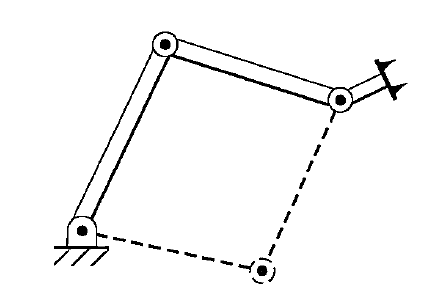
\includegraphics[width=.8\textwidth]{rigidbody/fig/ik-multiple-solutions.png}
    \caption{Πολλαπλότητα λύσεων}
    \label{fig:ik-multiple-solutions}
\end{figure}

Ένα σημαντικό πρόβλημα που έχει να κάνει με τις δυνατότητες του συγκεκριμένου συστήματος καταγραφής είναι ότι το η πληροφορία που σου παρέχει μπορεί να μην αρκεί για να περιγράψει σωστά την διάταξη. Δηλαδή, αν υποθέσουμε ότι έχουμε μια άρθρωση με έξι βαθμούς ελευθερίας (τρεις περιστροφές και τρεις μετατοπίσεις) τότε για να επιλυθεί το σύστημα απαιτούνται τουλάχιστον τρία σημεία πάνω στο τμήμα, που να μην είναι συγγραμμικά μεταξύ τους. Για αυτό το λόγο τα καλά συστήματα όπως είναι το \eng{Vicon} καταγράφουν πολλαπλές θέσεις σε κάθε τμήμα του σώματος.
 
%%%%%%%%%%%%%%%%%%%%%%%%%%%%%%%%%%%%%%%%%%%%%%%%%%%%%%%%%%%%%%%%%%%%%%%%%%%%%%%%
\section{Δυναμική}

Αφού έχει γίνει η ανάλυση της κινηματικής μπορεί κανείς να κάνει ένα βήμα πιο πέρα και να εξάγει σημαντικά συμπεράσματα για το μοντέλο, όπως είναι οι δυνάμεις και οι ροπές που ασκούνται στις αρθρώσεις για την παραγωγή της δοσμένης κίνησης. Η δυναμική είναι η μελέτη του υπολογισμού των δυνάμεων και των ροπών για δεδομένες τροχιές, ταχύτητες και επιταχύνσεις με βάση τον δεύτερο νόμο του Νεύτωνα.

Υπάρχουν διάφοροι μέθοδοι για των υπολογισμό των δυνάμεων και των ροπών. Μια κατηγορία είναι η αναλυτική μέθοδος, η οποία σου δίνει όλη την πληροφορία της διάταξης. Οι πράξεις που απαιτούνται για τον υπολογισμό μιας χρονικής στιγμής όσον αφορά της προσθέσεις και τους πολλαπλασιασμούς είναι της τάξης $O(n^4)$, όπου $n$ οι βαθμοί ελευθερίας της διάταξης. Από την άλλη έχουμε αναδρομικές μεθόδους όπως είναι η \eng{Iterative Newton-Euler}, που είναι πιο αποδοτικές και επιτυγχάνουν πολυπλοκότητα της τάξεως $O(n)$.

Σκοπός όλων των μεθόδων είναι η επίλυση της γενικευμένης δυναμικής εξίσωσης \ref{equ:dynamics-equation} που περιγράφει την διάταξη.

\begin{equation}
    M(q) \cdot \ddot{q} + V(q, \dot{q}) + G(q) + F(q, \dot{q}) = \tau
    \label{equ:dynamics-equation}
\end{equation}

Όπου $\theta$ είναι η γενικευμένη συντεταγμένη των αρθρώσεων και είναι ένα διάνυσμα στήλης μεγέθους $n \times 1$ όσο είναι οι βαθμοί ελευθερίας του συστήματος. Ο $M(q)$ είναι ο πίνακας αδράνειας του συστήματος διαστάσεων $n \times n$ και εξαρτάται από το $q$ (την γενικευμένη θέση). Το διάνυσμα στήλης $V(q, \dot{q})$ μεγέθους $n \times 1$ συμβολίζει τις φυγόκεντρες δυνάμεις και τις δυνάμεις \eng{Coriolis}, που εξαρτιούνται από το τετράγωνο της ταχύτητας και το γινόμενο των συζευγμένων ταχυτήτων αντίστοιχα. Το διάνυσμα στήλης $G(q)$ μεγέθους $n \times 1$ είναι η βαρύτητα που δρα πάνω στα διάφορα τμήματα της διάταξης. Το διάνυσμα $F(q, \dot{q})$ μεγέθους $n \times 1$ έχει να κάνει με τις εξωτερικές δυνάμεις, όπως είναι οι τριβές για παράδειγμα. Τέλος, από την άλλη μεριά της εξίσωσης έχουμε τις γενικευμένες δυνάμεις και ροπές που πρέπει να ασκηθούν στις αρθρώσεις για να παραχθεί η κίνηση με μέγεθος και είναι διάστασης $n \times 1$.

%%%%%%%%%%%%%%%%%%%%%%%%%%%%%%%%%%%%%%%%%%%%%%%%%%%%%%%%%%%%%%%%%%%%%%%%%%%%%%%%
\subsection{Επίλυση με τον Αναδρομικό Αλγόριθμο}

Η περιγραφή των εξισώσεων του αλγορίθμου eng{Iterative Newton-Euler} προϋποθέτουν την γνώση των θέσεων, των ταχυτήτων και των επιταχύνσεων $(q, \dot{q}, \ddot{q})$ για όλες τις αρθρώσεις. Επίσης, είναι απαραίτητη και η γνώση της κατανομής της μάζας των τμημάτων του μοντέλου που υπολογίζονται ως προς το κέντρο μάζας. Ο αλγόριθμος αποτελείται από δύο βήματα. Το πρώτο βήμα ξεκινώντας από την βάση μέχρι την άκρη (τελευταία άρθρωση στην αλυσίδα) του μοντέλου υπολογίζει τις ταχύτητες και τις επιταχύνσεις που διαδίδονται, αλλά και τις δυνάμεις και τις ροπές του κέντρου μάζας με βάση τις εξισώσεις \ref{equ:iterative-NE-first}. Το δεύτερο βήμα ξεκινώντας ανάποδα από την άκρη μέχρι την βάση υπολογίζει τις δυνάμεις και τις ροπές στις αρθρώσεις με βάση τις εξισώσεις \ref{equ:iterative-NE-second}.

\begin{figure}[H]
    \centering
    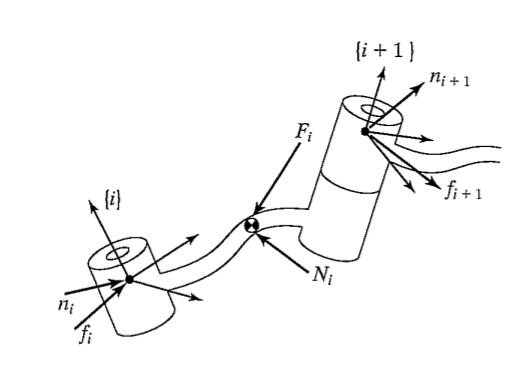
\includegraphics[width=.8\textwidth]{rigidbody/fig/force-balance.png}
    \caption{Διάγραμμα δυνάμεων ισορροπίας}
    \label{fig:force-balance}
\end{figure}

Η πρώτη αναδρομή περιγράφεται από τις εξής σχέσεις για $i : 0 \rightarrow n-1$:

\begin{equation}
    \begin{aligned}
        ^{i+1}\omega_{i+1} = {}^{i+1}R_i \cdot {}^i\omega_i +
        \dot{q}_{i+1} \times {}^{i+1}\hat{Z}_{i+1}\\[10pt]
        ^{i+1}\dot{\omega}_{i+1} = {}^{i+1}R_i \cdot {}^i\dot{\omega}_i +
        {}^{i+1}R_i \cdot {}^i\omega_i \times \dot{q}_{i+1} \cdot
        {}^{i+1}\hat{Z}_{i+1} + \ddot{q}_{i+1} \cdot
        {}^{i+1}\hat{Z}_{i+1}\\[10pt]
        ^{i+1}\dot{u}_{i+1} = {}^{i+1}R_i \cdot (^i\dot{\omega}_i \times
        {}^iP_{i+1} + {}^i\omega_i \times (^i\omega_i \times {}^iP_{i+1}) +
        {}^i\dot{u}_i)\\[10pt]
        ^{i+1}\dot{u}_{C_{i+1}} = {}^{i+1}\dot{\omega}_{i+1} \times
        {}^{i+1}P_{C_{i+1}} + {}^{i+1}\omega_{i+1} \times (^{i+1}\omega_{i+1}
        \times {}^{i+1}P_{C_{i+1}}) + {}^{i+1}\dot{u}_{i+1}\\[10pt]
        ^{i+1}F_{i+1} = m_{i+1} \cdot {}^{i+1}\dot{u}_{C_{i+1}}\\[10pt]
        ^{i+1}N_{i+1} = {}^{C_{i+1}}I_{i+1} \cdot {}^{i+1}\dot{\omega}_{i+1} +
        {}^{i+1}\omega_{i+1} \times {}^{C_{i+1}}I_{i+1} \cdot {}^{i+1}\omega_{i+1}
    \end{aligned}
    \label{equ:iterative-NE-first}
\end{equation}

Η δεύτερη αναδρομή περιγράφεται από τις εξής σχέσεις για $i : n \rightarrow 1$:

\begin{equation}
    \begin{aligned}
        ^if_i = {}^{i}R_{i+1} \cdot {}^{i+1}f_{i+1} + {}^iF_i\\[10pt]
        ^in_i = {}^iN_i + {}^iR_{i+1} \cdot {}^{i+1}n_{i+1} + {}^iP_{C_i} \times
        {}^iF_i + {}^iP_{i+1} \times {}^iR_{i+1} \cdot {}^{i+1}f_{i+1}\\[10pt]
        \tau_i = {}^in^T_i \cdot {}^i\hat{Z}_i
    \end{aligned}
    \label{equ:iterative-NE-second}
\end{equation}



%%%%%%%%%%%%%%%%%%%%%%%%%%%%%%%%%%%%%%%%%%%%%%%%%%%%%%%%%%%%%%%%%%%%%%%%%%%%%%%%
\chapter{Μυοσκελετικό Σύστημα}

Σε αυτό το κεφάλαιο παρουσιάζεται η διαδικασία της δυναμικής σε μυοσκελετικά μοντέλα. Στόχος είναι να εκτιμηθούν οι δυνάμεις που παράγονται από τους μύες, που μετατρέπονται σε  ροπές, οι οποίες με την σειρά τους σε κίνηση που προέρχεται από την νευρική διέγερση των μυών. Η παραπάνω διαδικασία μπορεί να χωριστεί σε τέσσερα βήματα, την μυϊκή ενεργοποίση (\eng{muscle activation dynamics}), την μυϊκή συστολή (\eng{muscle contraction dynamics}), την μυοσκελετική γεωμετρία και τέλος την εξίσωσης της κίνησης, η οποία επιτρέπει την μετατροπή της ροπής των αρθρώσεων σε κίνηση. Η διαδικασία περιγράφεται εποπτικά από την εικόνα \ref{fig:muscle-excitation-force}.

\begin{figure}[H]
    \centering
    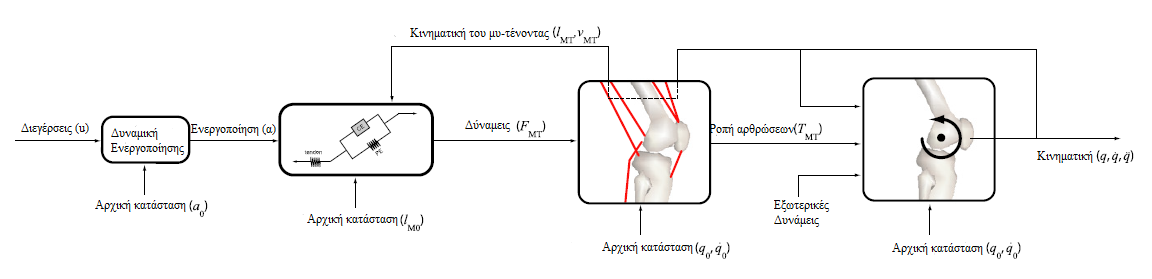
\includegraphics[width=1.0\textwidth]{musculoskeletal/fig/muscle-excitation-force.png}
    \caption{Στάδια από την διέγερση έως την παραγωγή της κίνησης\cite{erdemir07}}
    \label{fig:muscle-excitation-force}
\end{figure}

Στο παρόν κεφάλαιο θα ξεκινήσουμε με μια εισαγωγή στην φυσιολογία του μυ. Στην συνέχει θα γίνει ανάλυση της δυναμικής συμπεριφοράς της ενεργοποίησης και θα δοθεί μια μαθηματική διατύπωση. Έπειτα θα γίνει εισαγωγή στο μοντέλο του μυ και συγκεκριμένα στα \eng{Hill-Type} μοντέλα. Τέλος θα δοθεί εξήγηση πώς η τοποθεσία του μυ επηρεάζει την δυναμική του συμπεριφορά και πως αυτό μοντελοποιείται.

%%%%%%%%%%%%%%%%%%%%%%%%%%%%%%%%%%%%%%%%%%%%%%%%%%%%%%%%%%%%%%%%%%%%%%%%%%%%%%%%
\section{H Φυσιολογία του Μυ}

%%%%%%%%%%%%%%%%%%%%%%%%%%%%%%%%%%%%%%%%%%%%%%%%%%%%%%%%%%%%%%%%%%%%%%%%%%%%%%%%
\subsection{Δομή}

Ο σκελετικός μυς είναι μια συλλογή από μυϊκά κύτταρα (μυϊκές ίνες) \cite{zirinoglou}. Ο αριθμός των μυϊκών ινών εξαρτάται από το μέγεθος του μυός και ποικίλει από μερικές εκατοντάδες έως αρκετές χιλιάδες ίνες. Ολόκληρος ο μυς καλύπτεται και προστατεύεται από ένα συνδετικό περιτοναϊκό ιστό, ο όποιος περιβάλλει κάθε μυϊκή ίνα, τένοντα, οστό, νεύρο και αγγείο. Ο μυς διαιρείται περεταίρω σε αρκετές μυϊκές δεσμίδες. Κάθε δέσμη περιέχει περίπου εκατό μυϊκές ίνες. Κάθε ίνα έχει διάμετρο 50μ\eng{m} με 100μ\eng{m} (χιλιοστά του χιλιοστόμετρου), μήκος 2 με 6 εκατοστά και περιέχει περισσότερα από 1000μ\eng{m} με 2000μ\eng{m} μυϊκά ινίδια, τα οποία με την σειρά τους περιέχουν μια αλυσίδα από σαρκομέριο. Κάθε μυϊκό ινίδιο αποτελείται από αρκετούς τύπους πρωτεϊνών.

\begin{figure}[H]
    \centering
    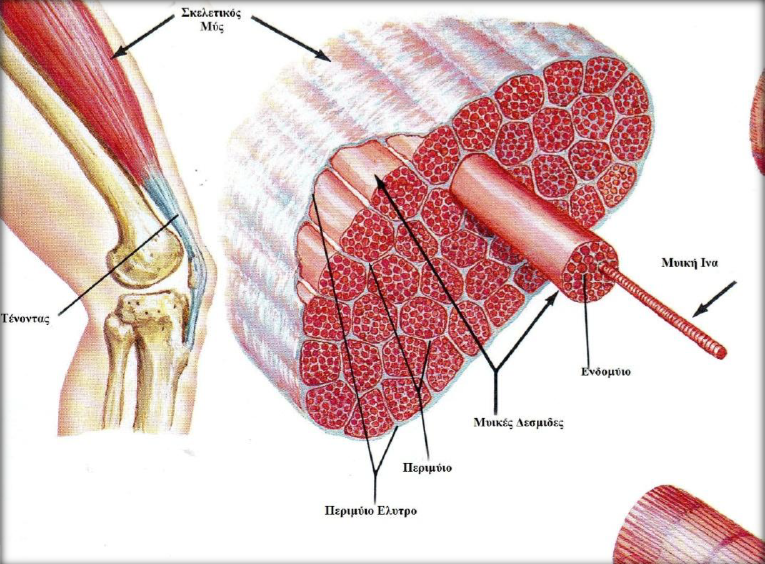
\includegraphics[width=.8\textwidth, height=0.5\textheight]{musculoskeletal/fig/muscle-fysiology.png}
    \caption{Σκελετικός μυς: ανατομική περιγραφή\protect\footnotemark}
    \label{fig:muscle-fysiology}
\end{figure}

Το σαρκομέριο είναι η συσταλτή μονάδα του μυϊκού ινιδίου και αποτελείται από επικαλυπτόμενες εγκάρσιες γέφυρες ακτίνης και μυοσίνης. Το σαρκομέριο δίνει την δυνατότητα στον μυ να συσπάται και να χαλαρώνει. Όταν ο μυς συσπάται, τα λεπτά νημάτια ακτίνης και μυοσίνης ολισθαίνουν μεταξύ τους και ο μυς βραχύνεται. Όταν ο μυς χαλαρώνει, οι εγκάρσιες γέφυρες ολισθαίνουν ήπια και ξεχωριστά, και ο μυς επιστρέφει στο μήκος ηρεμίας.

\begin{figure}[H]
    \centering
    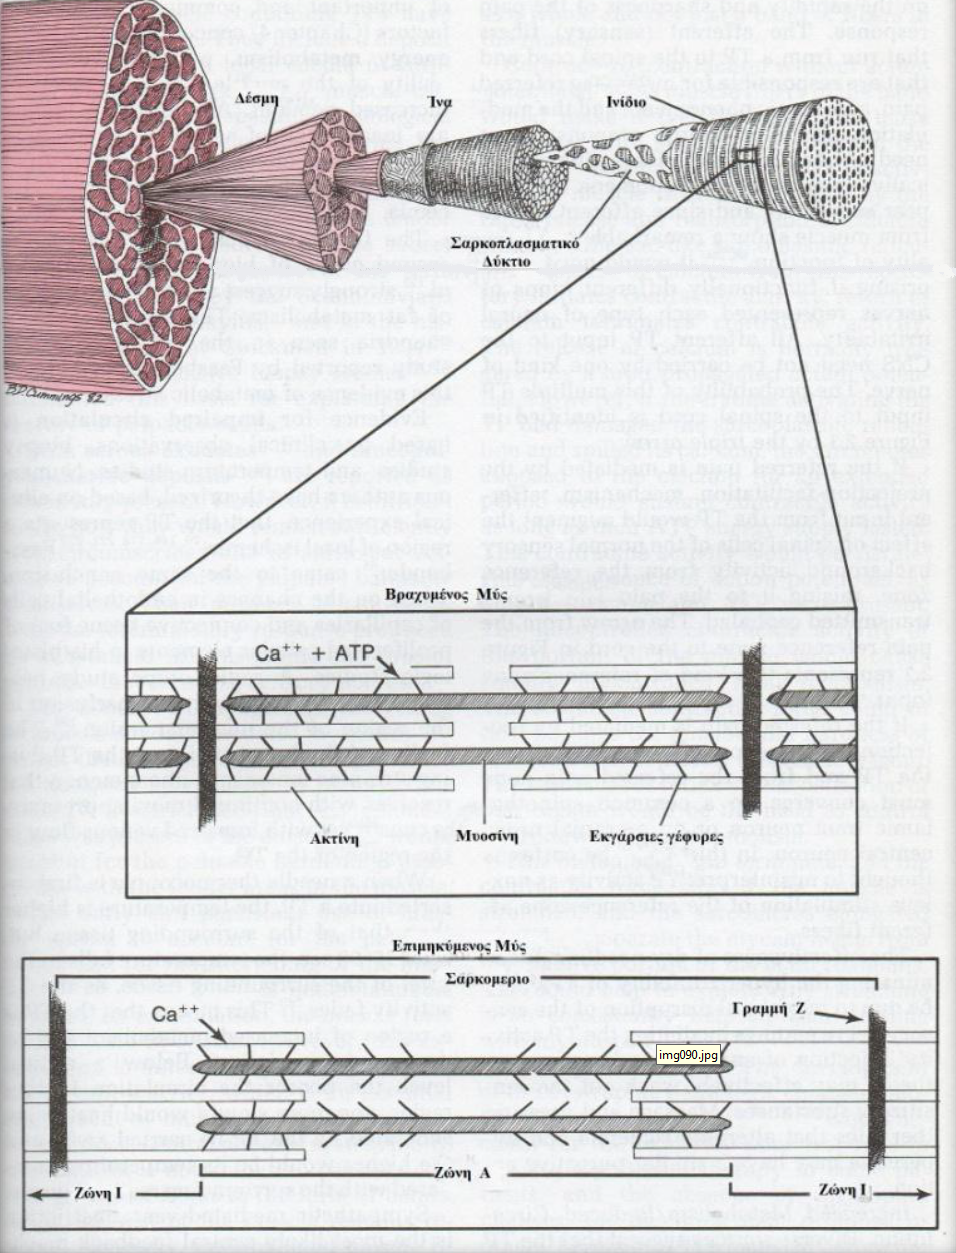
\includegraphics[width=.8\textwidth, height=0.5\textheight]{musculoskeletal/fig/muscle-fysiology2.png}
    \caption{Δομή και συσταλτικός μηχανισμός του φυσιολογικού σκελετικού μυός\protect\footnotemark}
    \label{fig:muscle-fysiology2}
\end{figure}
\footnotetext{Εικόνα από το βιβλίο \eng{Travell \& Simons} 1999}

%%%%%%%%%%%%%%%%%%%%%%%%%%%%%%%%%%%%%%%%%%%%%%%%%%%%%%%%%%%%%%%%%%%%%%%%%%%%%%%%
\subsection{Σαρκοπλασματικό Δίκτυο}

Το σαρκοπλασματικό δίκτυο είναι ένα δίκτυο σωληνοειδούς μορφής το οποίο εκτείνεται σε ολόκληρο τον μυ. Τα επιμήκη σαρκοπλασματικά σωληνάρια καταδύονται σε μια σχετικά μεγάλη τελική δεξαμενή σε οποιαδήποτε άκρη του σαρκομερίου. Δυο τελικές δεξαμενές σε συνδυασμό με ένα εγκάρσιο σωληνάριο (\eng{T-tubule}) σχηματίζουν μια τριάδα. Η τριάδα είναι τοποθετημένη σε καίρια θέση δίπλα από το τμήμα της μυϊκής ίνας, το οποίο παράγει τις απαραίτητες δυνάμεις για την συστολή. Το εγκάρσιο σωληνάριο παίζει ένα σημαντικό ρόλο στη διέλευση του δυναμικού ενέργειας βαθιά μέσα στον μυ. Ο ρόλος του σαρκοπλασματικου δικτύου είναι να αποθηκεύει $Ca^{2+}$, το οποίο είναι απαραίτητο για την συστολή του μυός.

\begin{figure}[H]
    \centering
    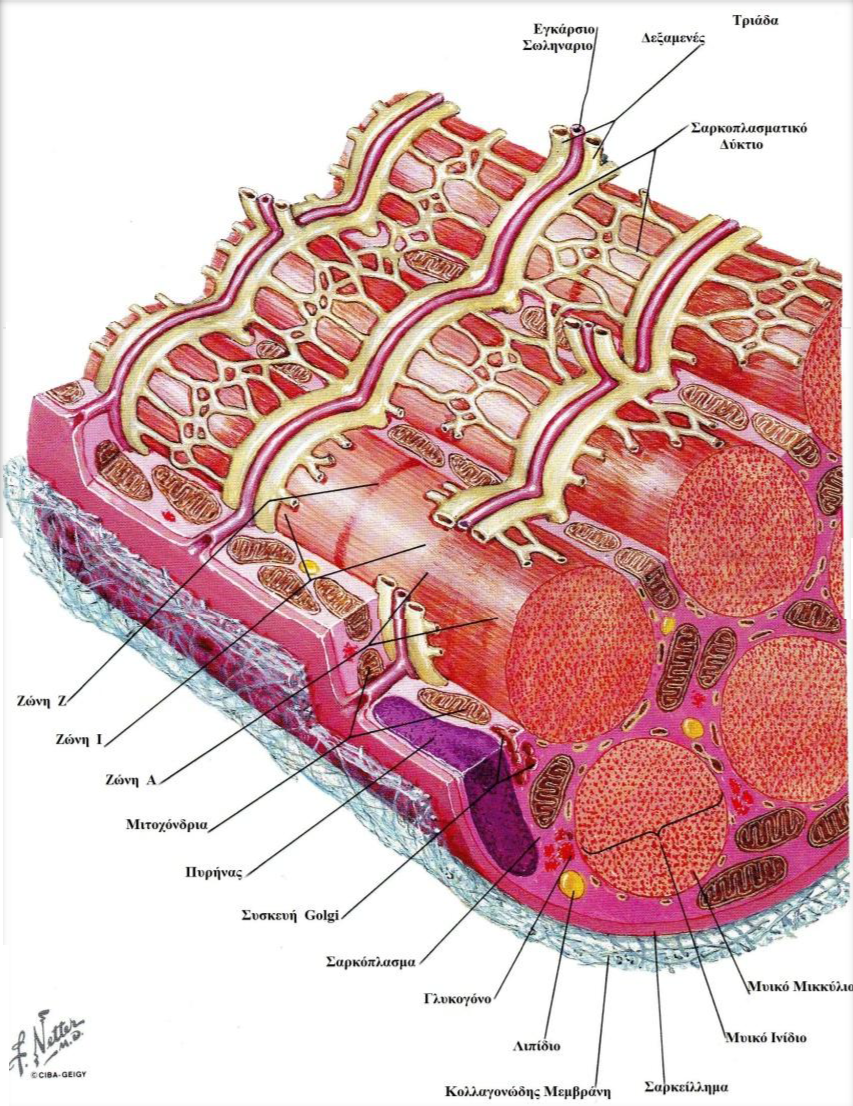
\includegraphics[width=.7\textwidth, height=0.6\textheight]{musculoskeletal/fig/muscle-fysiology3.png}
    \caption{Σαρκοπλασματικό δίκτυο\protect\footnotemark}
    \label{fig:muscle-fysiology3}
\end{figure}
\footnotetext{Εικόνα από το βιβλίο \eng{Netter} 1987}

%%%%%%%%%%%%%%%%%%%%%%%%%%%%%%%%%%%%%%%%%%%%%%%%%%%%%%%%%%%%%%%%%%%%%%%%%%%%%%%%
\subsection{Το Νευρικό Σύστημα}

Η κύρια εργασία του κινητικού νευρικού συστήματος είναι να ελέγχει και να συντονίζει τη λειτουργία των συσταλτών στοιχείων σε όλους τους μύες ταυτόχρονα, έτσι ώστε να εφαρμόζεται η κατάλληλη τάση στον σκελετό για να παραχθεί η επιθυμητή κίνηση.

\begin{figure}[H]
    \centering
    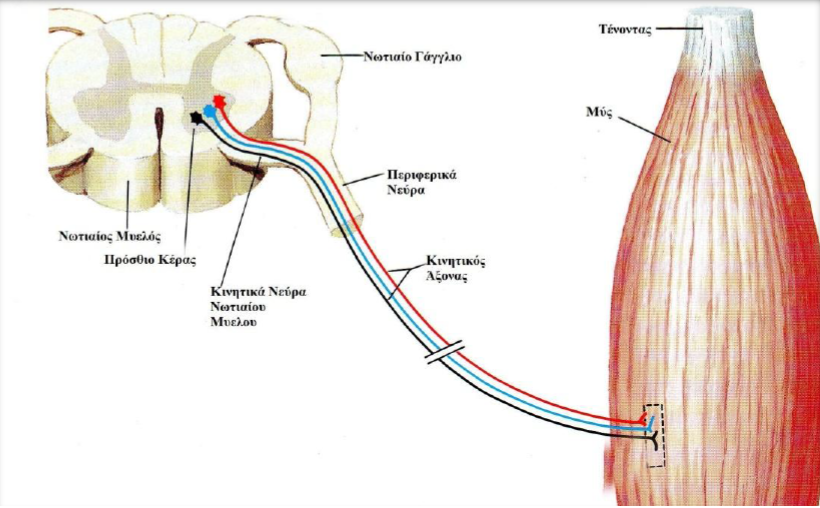
\includegraphics[width=.8\textwidth]{musculoskeletal/fig/muscle-fysiology4.png}
    \caption{Κινητικοί νευρώνες του νωτιαίου μυελού\protect\footnotemark}
    \label{fig:muscle-fysiology4}
\end{figure}
\footnotetext{Εικόνα από το βιβλίο \eng{Netter} 1987}

Ο κινητικός νευρώνας θεωρείται ως η λειτουργική μονάδα του κινητικού νευρικού συστήματος. Τα κυτταρικά σώματα των κινητικών νευρώνων είναι στοιβαγμένα σε έναν κινητικό πυρήνα μέσα στο κοιλιακό τμήμα της σπονδυλικής στήλης. Ο άξονας κάθε κινητικού νευρώνα εκφύεται από την σπονδυλική στήλη διαμέσου μιας κοιλιακής ρίζας (ή ενός κρανιακού νεύρου από το εγκεφαλικό στέλεχος) και διαιρείται σε μικρότερους κλάδους περιφερικών νεύρων μέχρι να εισέλθει στον μυ που ελέγχεται από αυτό το νεύρο. Οι άξονες των κινητικών νευρώνων είναι εμμύελοι. Δύνανται έτσι να μεταδίδουν δυναμικά ενέργειας με υψηλή ταχύτητα, επιτρέποντας ώσεις από το κεντρικό νευρικό σύστημα να μεταφέρονται στις μυοσκελετικές ίνες με ελάχιστη καθυστέρηση. Με την άφιξη του στο μυ, ο άξονας του κινητικού νευρώνα διακλαδίζεται πολλαπλά, με κάθε διακλάδωση να σχηματίζει μια απλή σύναψη με μια μυϊκή ίνα.

Το απόλυτο μυϊκό μήκος και οι αλλαγές του μυϊκού μήκους ανιχνεύονται από διατατικούς αισθητήρες που είναι στρωμένοι μέσα στο μυ. Οι αισθητήρες αυτοί αποτελούνται από απολήξεις προσαγωγών νευρικών ινών που είναι τυλιγμένες γύρω από τροποποιημένες μυϊκές ίνες, αυτή η δομή ονομάζεται μυϊκή άτρακτος. Είναι απαραίτητες για την γνώση της θέσης και της κίνησης των μελών, αλλά επίσης συντελεί στο λεπτό κινητικό έλεγχο.

\begin{figure}[H]
    \centering
    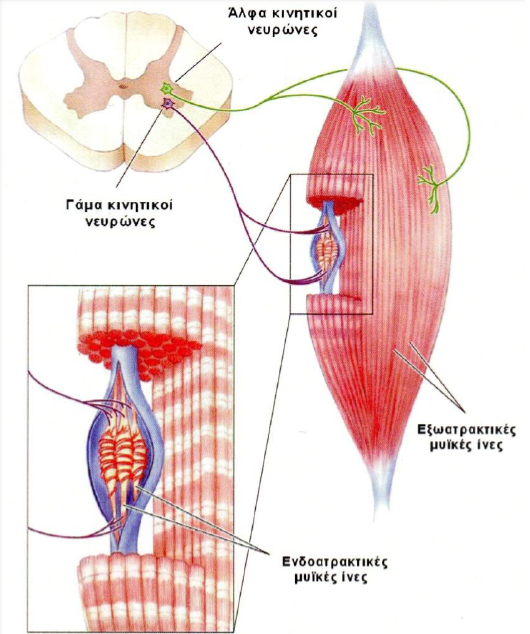
\includegraphics[width=.8\textwidth, height=0.5\textheight]{musculoskeletal/fig/muscle-fysiology5.png}
    \caption{Κινητική μονάδα (μυϊκή άτρακτος)}
    \label{fig:muscle-fysiology5}
\end{figure}

Οι τροποποιημένες μυϊκές ίνες που ένγκεται μέσα στην άτρακτο είναι γνωστές ως ενδοατράκτικες ίνες, ενώ οι μυοσκελετικές ίνες, οι οποίες αποτελούν την πλειονότητα των ινών ενός μυός και παράγουν δύναμη και κίνηση, ονομάζονται εξωατράκτιες ίνες. Μέσα στην μυϊκή άτρακτο υπάρχουν δύο διατατικοί αισθητήρες. Το ένα είδος ανταποκρίνεται άριστα στο πόσο ο μυς έχει διαταθεί και το άλλο στο μέγεθος και στην ταχύτητα διάτασης. Πρωταγωγείς (τύπου Ια) και δευτεραγωγείς (τύπου ΙΙ) κεντρομόλες ίνες ανέρχονται από τις μυϊκές ατράκτους, συνάπτονται με άλφα ή γάμα κινητικούς νευρώνες αντίστοιχα και διευκολύνουν τη σύσπαση των εξωατρακτικων και ενδοατρακτικων ινών.

%%%%%%%%%%%%%%%%%%%%%%%%%%%%%%%%%%%%%%%%%%%%%%%%%%%%%%%%%%%%%%%%%%%%%%%%%%%%%%%%
\subsection{\texorpdfstring{Το Αισθητήριο Όργανο \eng{Golgi}}{}}

Το όργανο του \eng{Golgi} βρίσκεται κοντά στην μυοτενόντια σύναψη, τυλίγεται γύρω από τα άκρα των εξωατρακτικών ινών του μυός και είναι ευαίσθητο στην τάση που προκαλείται στον μυ από παθητική διάταση ή από ενεργητική σύσπαση του. Το όργανο του \eng{Golgi} είναι ένας προστατευτικός μηχανισμός που αναστέλλει την σύσπαση του μυός στον όποιο βρίσκεται. Η ουδός πυροδότησης είναι πολύ χαμηλή (ενεργοποιείται εύκολα), μετά από ενεργητική μυϊκή σύσπαση και πολύ υψηλή, μετά από μια παθητική διάταση. Όταν αναπτύσσεται υπερβολική τάση στον μυ, το όργανο του \eng{Golgi} πυροδοτεί, αναστέλλει τη δραστηριότητα του άλφα κινητικού νευρώνα και μειώνει την τάση του μυός. Κατά την διάρκεια των διαδικασιών της διάτασης, η τάση στον τένοντα καθορίζει αν το κάθε σαρκομέριο του μυός είναι επιμηκυμένο.

Κατά την διάρκεια όμως της ισοτονικής και της ισομετρικής συστολής του μυός η κατάσταση διαφοροποιείται. Ενώ σταματά να διατείνεται η μυϊκή άτρακτος, το τενόντιο όργανο συνεχίζει να βρίσκεται σε διάταση και στην πραγματικότητα ο ρυθμός της πυροδότησης του αυξάνεται σε όλη τη διάρκεια της συστολής. Ο δυναμικός κώδικας του ενάντιου οργάνου σηματοδοτεί το ρυθμό αύξησης της έντασης κατά την διάρκεια της συστολής και το ρυθμό της μείωσης της διέγερσης κατά την διάρκεια της χαλάρωσης. Το πρότυπο διέγερσης των τενόντιων οργάνων κατά την διάρκεια της συστολής δείχνει ότι ο κύριος ρόλος τους είναι να ελέγχουν το ρυθμό της αλλαγής της έντασης σε έναν συστελλόμενο μυ καθώς σηματοδοτούν το ποσοστό της έντασης που υπάρχει σε έναν ισομετρικά συστελλόμενο μυ.

%%%%%%%%%%%%%%%%%%%%%%%%%%%%%%%%%%%%%%%%%%%%%%%%%%%%%%%%%%%%%%%%%%%%%%%%%%%%%%%%
\section{Μοντέλο του Μυ}

Ένα μοντέλο του μυ περιγράφει την διαδικασία παραγωγής της δύναμης κάτω από μια νευρική διέγερση και μπορούν να καταταχθούν σε μικροσκοπικά και μακροσκοπικά μοντέλα. Τα μικροσκοπικά μοντέλα ανήκουν στην κατηγορία \eng{Huxley-Type} προς τιμή του \eng{Huxley 1957}, ενώ το πιο διάσημο μακροσκοπικό μοντέλο είναι το \eng{Hull-Type} προς τιμή του \eng{Hill 1938}. Τα δύο αυτά μοντέλα χρησιμοποιούνται ευρέως στην επιστημονική κοινότητα. Όσον αφορά τα μοντέλα \eng{Hill-Type} είναι καταλληλότερα σε εφαρμογές προσομοίωσης, γιατί είναι πιο απλά και έχουν λιγότερους παραμέτρους που πρέπει να προσδιορισθούν. Για αυτό το λόγο, η ανάλυση που θα γίνει στην συνέχεια αφορά την δεύτερη κατηγορία μοντέλων.

%%%%%%%%%%%%%%%%%%%%%%%%%%%%%%%%%%%%%%%%%%%%%%%%%%%%%%%%%%%%%%%%%%%%%%%%%%%%%%%%
\subsection{Μοντέλο Ενεργοποίησης}

Η αλληλεπίδραση μεταξύ ινιδίων μυοσίνης και ακτίνης ενεργοποιείται, όταν το μυϊκό κύτταρο δεχτεί ένα κατάλληλο σήμα από το νευρικό σύστημα. Το σήμα πυροδοτεί ένα δυναμικό ενέργειας στην κυτταρική μεμβράνη του κυττάρου. Αυτή η ηλεκτρική διέγερση διαδίδεται κατά μήκος μιας σειράς μεμβρανικών σωλήνων, τα εγκάρσια σωληνάρια, και το σήμα μεταφέρεται στο σαρκοπλασματικό δίκτυο, το οποίο περιέχει υψηλή συγκέντρωση ασβεστίου. Σαν αντίδραση στην εισερχόμενη ηλεκτρική διέγερση, μεγάλο ποσό $Ca^{+2}$ απελευθερώνεται στο κυτταροδιάλυμα μέσω ιοντικών διαύλων της μεμβράνης του σαρκοπλασματικού δικτύου που ανοίγουν εξαιτίας της ηλεκτρικής διέγερσης.

Το ιόν του ασβεστίου αλληλεπιδρά με εξειδικευμένες πρωτεΐνες που συνδέονται ισχυρά με τα ινίδια ακτίνης. Μια από αυτές τις πρωτεΐνες είναι η τροπομυοσίνη, ένα άκαμπτο ραβδόμορφο πρωτεϊνικό μόριο που προσδένεται στο αυλάκι της έλικας της ακτίνης και δεν την αφήνει να αντιδράσει με τις κεφαλές μυοσίνης. Η άλλη είναι η τροπονίνη, ένα πρωτεϊνικό σύμπλοκο που περιλαμβάνει μια πρωτεΐνη ευαίσθητη στο ασβέστιο, την τροπονίνη \eng{C}. Όταν αυξηθεί η συγκέντρωση του ασβεστίου στο κυτταροδιάλυμα, το ιόν ασβεστίου προσδένεται στη τροπονίνη και προκαλεί μια αλλαγή στο σχήμα της και έτσι οι κεφαλές μυοσίνης μπορούν να προσδεθούν στο ινίδιο ακτίνης και να αρχίσει η συστολή.

Η αύξηση του $Ca^{+2}$ στο κυτταροδιάλυμα σταματά αμέσως μετά τη διακοπή του νευρικού σήματος, επειδή το ιόν του ασβεστίου αντλείται γρήγορα πίσω στο σαρκοπλασματικό δίκτυο. Μόλις η συγκέντρωση ασβεστίου επανέλθει σε επίπεδα ηρεμίας, η τροπονίνη και η τροπομυοσίνη επιστρέφουν στις αρχικές τους θέσεις και σταματούν τη συστολή.

Ένας μυς δεν μπορεί να παράξει δύναμη ή να χαλαρώσει ακαριαία. Πειραματικά έχει αποδειχτεί ότι η καθυστέρηση από την στιγμή της διέγερσης μέχρι την ανάπτυξη της δύναμης ξεκινά από 5\eng{ms} για την παραγωγή της δύναμης από τους γρήγορους μύες του οφθαλμού, και από 40\eng{ms} έως 50\eng{ms} από μύες με πιο μεγάλα ποσοστά βραδείας σύσπασης \cite{zajac89}. Η διαδικασία της χαλάρωσης είναι πιο αργή με αποτέλεσμα να χρειαστεί περισσότερο χρόνο. Η ενεργοποίηση των μυών μπορεί να μοντελοποιηθεί με μια διαφορική εξίσωση πρώτης τάξεως.

\begin{equation}
    \begin{gathered}
        \hat{a} = \frac{a - a_{min}}{1 - a_{min}}\\[10pt]
        \frac{da}{dt} = \frac{u - \hat{a}}{\tau (\hat{a}, u)}\\[10pt]
        \tau (\hat{a}, u) =
        \begin{cases}
            t_{act} \cdot (0.5 +1.5 \cdot \hat{a}), & u > \hat{a} \\
            t_{deact}/(0.5 +1.5 \cdot \hat{a}), & u \leq \hat{a}
        \end{cases}
    \end{gathered}
    \label{equ:activation-dynamics}
\end{equation}

Όπου $u$ η διέγερση και $a$ η ενεργοποίηση. Το παραπάνω μοντέλο παρουσιάστηκε από \cite{millard13} και ακολουθεί με μικρές αλλαγές τα μοντέλα \cite{thelen03, winters95}, όπου η χρονική μεταβολή $\frac{da}{dt}$ ισούται με την διαφορά $u - a$ δια μια συνάρτηση. Η διαφορά του μοντέλου από τα προηγούμενα είναι ο παράγοντας $\hat{a}$ που κάνει την εξίσωση \ref{equ:activation-dynamics} κατάλληλη για προσομοιώσεις, κρατώντας το αποτέλεσμα στα όρια $(0.01, 1), a_{min} = 0.01$.

%%%%%%%%%%%%%%%%%%%%%%%%%%%%%%%%%%%%%%%%%%%%%%%%%%%%%%%%%%%%%%%%%%%%%%%%%%%%%%%%
\subsection{Μοντέλο Συστολής}

Αφότου έχει εκτιμηθεί η ενεργοποίση $a$ του μυ, το επόμενο βήμα είναι ο προσδιορισμός της δύναμης που θα παράξει. Όπως αναφέραμε τα μοντέλα \eng{Huxley-Type} περιγράφονται από πολύπλοκες εξισώσεις, με πολλούς παραμέτρους, που πρέπει στην πορεία της προσομοίωσης να ολοκληρωθούν, με αποτέλεσμα να έχουν μεγάλο υπολογιστικό κόστος.

\begin{figure}[H]
    \centering
    \begin{subfigure}[Η]{.5\textwidth}
        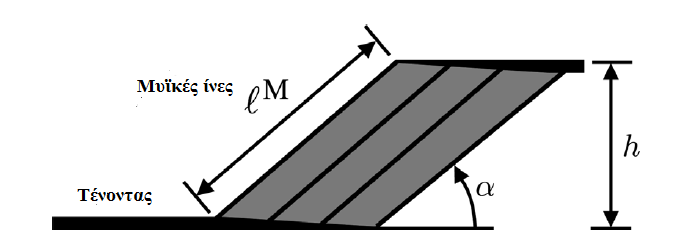
\includegraphics[width=\textwidth]{musculoskeletal/fig/simple-muscle-model.png}
        \caption{Απλοποιημένο μοντέλο\cite{millard13}}
        \label{fig:simple-mascle-model}
    \end{subfigure} ~
    \begin{subfigure}[Η]{.4\textwidth}
        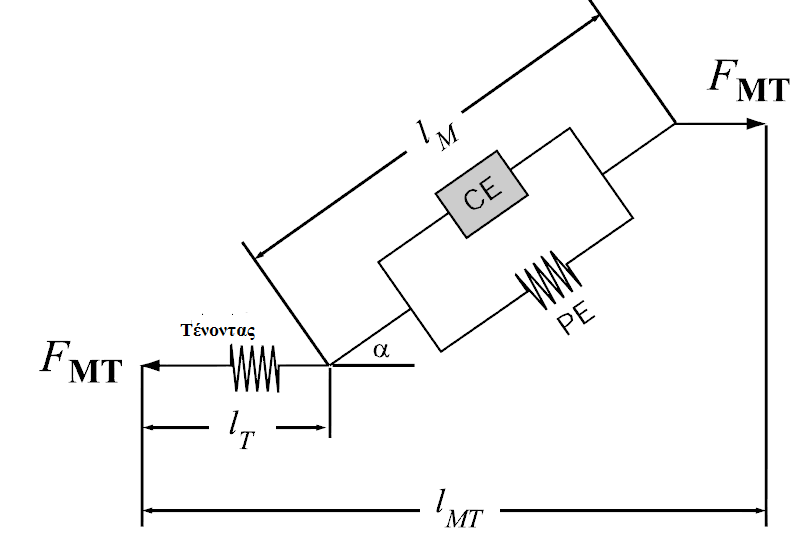
\includegraphics[width=\textwidth]{musculoskeletal/fig/muscle-model.png}
        \caption{Μαθηματικό μοντέλο\cite{erdemir07}}
        \label{fig:muscle-model}
    \end{subfigure}
    \caption{Μοντέλο του μυ}
\end{figure}
%\footnotetext{Εικόνες από την δημοσίευση \cite{millard13}}

Όπως φαίνεται στην εικόνα \ref{fig:simple-mascle-model} οι μυικές ίνες συνδέονται με τον τένοντα υπό μια γωνιά α (\eng{pennation angle}). Η μοντελοποίηση της συστολής αποτελείται από τρία μέρη: το παθητικό (\eng{passive element}) που είναι μια δύναμη που ασκείται όταν ο μυς τεντωθεί πάνω από ένα συγκεκριμένο όριο, ο συστολικός μηχανισμός (\eng{contractile element}) που αφορά την παραγωγή της κύριας μυικής δύναμης και το σειριακό μέρος που έχει να κάνει με τις δυνάμεις που ασκούνται από το τένοντα.

Πριν περιγράψουμε τις συναρτήσεις, μπορούμε να δούμε την καμπύλη κανονικοποιημένης δύναμης σε σχέση με το μήκος του μυ \ref{fig:active-force-legnth}. Στον άξονα \eng{x} έχουμε το κανονικοποιημένο μήκος με βάση το βέλτιστο μήκος του μυ $l^{M}_{o}$ (\eng{optimal fiber length}), ενώ στο άξονα \eng{y} έχουμε την κανονικοποιημένη δύναμη με βάση την μέγιστη ισομετρική δύναμη $f^{M}_{o}$ (\eng{maximum isometric force}). Οι καμπάνες συμβολίζουν την δύναμη που παράγει ο μυς και διαφοροποιούνται για διαφορετικές τιμές ενεργοποίησης $a$, που κυμαίνονται από $a_{min}$ μέχρι 1. Όταν το μήκος του μυ βρίσκεται σε μικρότερη ή μεγαλύτερη τιμή από την $l^{M}_{o}$ δεν μπορεί να παράξει την μέγιστη δύναμη, εξαιτίας της μειωμένης επικάλυψης μεταξύ της ακτίνης και της μυοσίνης. Πρέπει να προσέξουμε ότι το βέλτιστο της καμπάνας δεν βρίσκεται για $l = 100\%$ όσο μειώνεται η τιμή του \eng{a}. Επίσης, βλέπουμε ότι όταν ξεπεράσουμε ένα όριο επιμήκυνσης εμφανίζεται μια εκθετική δύναμη, που συμβολίζει την παθητική λειτουργία του μυ. Τέλος, η σύνθεση των δύο δυνάμεων παράγουν την καμπύλη δύναμη-μήκους για δεδομένη διέγερση.

\begin{figure}[H]
    \centering
    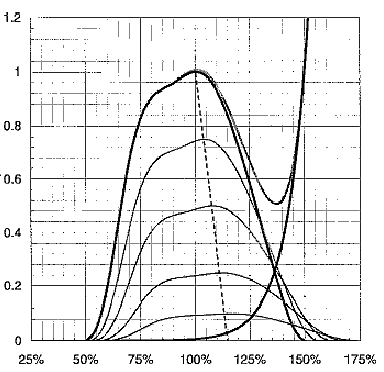
\includegraphics[width=.5\textwidth, height=.35\textheight]{musculoskeletal/fig/active-force-legnth.png}
    \caption{Καμπύλη δύναμη-μήκους για διαφορετικές τιμές ενεργοποιήσης\cite{buchanan04}}
    \label{fig:active-force-legnth}
\end{figure}
%\footnotetext{Εικόνα από την δημοσίευση \cite{buchanan04}}

\begin{figure}[H]
    \centering
    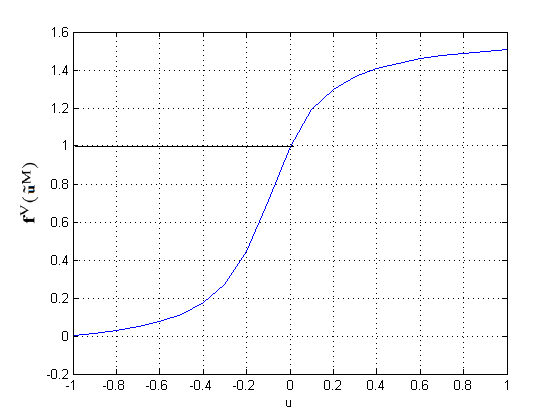
\includegraphics[width=.6\textwidth]{musculoskeletal/fig/force-velocity.png}
    \caption{Καμπύλη δύναμη-ταχύτητας}
    \label{fig:force-velocity}
\end{figure}
%\footnotetext{Εικόνα από την δημοσίευση \cite{millard13}}

Πέραν της σχέσης δύναμης-μήκους έχουμε και έναν άλλο παράγοντα που συνεισφέρει και σχετίζεται με την καμπύλη δύναμης-ταχύτητας \ref{fig:force-velocity}. Αυτή η δύναμη μοντελοποιεί την μη γραμμικότητα του ρυθμού επιμήκυνσης ή συστολής. Η δύναμη που παράγεται από τον μυ δίνεται από την εξίσωση της δύναμης.

\begin{equation}
    f^{M} = f^{M}_{o} \cdot (a \cdot f^{L}(\tilde{l}^{M}) \cdot f^{V}(\tilde{v}^{M}) + f^{PE}(\tilde{l}^{M}))
    \label{equ:muscle-force}
\end{equation}

Όπου οι παράμετροι $\tilde{l}^{M}, \tilde{l}^{V}$ συμβολίζουν τις κανονικοποιημένες ποσότητες, η $f^{L}$ συμβολίζει την δύναμη-μήκους μυ, η $f^{V}$ την δύναμη-ταχύτητας και η $f^{PE}$ την παθητική δύναμη. Δεν πρέπει να ξεχνάμε την επίδραση του τένοντα στην μοντελοποίηση, έχοντας ελαστικά χαρακτηριστικά λαμβάνοντας ρόλο της αντίδρασης στην δύναμη που ασκεί ο μυς. Αν θεωρήσουμε την μάζα του μυ αμελητέα χωρίς να εισάγουμε μεγάλο σφάλμα και γνωρίζοντας από την διάταξη \ref{fig:simple-mascle-model} ότι ο μυς βρίσκεται υπό γωνιά \eng{a} σε σχέση με τον τένοντα, τότε έχουμε την εξίσωση ισορροπίας με $f^{T}$ η δύναμη που ασκεί ο τένοντας.

\begin{equation}
    f^{M} \cdot \cos{a} - f^{M}_{o} \cdot f^{T}(\tilde{l}^{T}) = 0
    \label{equ:muscle-force-equilibrioum}
\end{equation}

Κατά την διαδικασία της ορθής δυναμικής η παραγωγή δύναμης από τον μυ εξαρτάται από $f^{M}(a, l^{m}, v^{M})$, οι οποίες πρέπει να προσδιοριστούν. Επίσης, η εξίσωση \ref{equ:muscle-force-equilibrioum} θα δώσει πολλαπλές λύσεις, για αυτό το λόγο η μοναδική λύση μπορεί να εξασφαλιστεί λύνοντας ως προς $\tilde{v}^{M}$.

\begin{equation}
    \tilde{v}^{M} = f^{V}_{inv} \bigg(\frac{f^{T}(\tilde{l}^{T})/\cos{a} - f^{PE}(\tilde{l}^{M})}{a \cdot f^{L}(\tilde{l}^{M})} \bigg)
    \label{equ:velocity-solution}
\end{equation}

Η παραπάνω εξίσωση, λαμβάνει απροσδιοριστία τιμή στις εξής τέσσερις περιπτώσεις: $a\rightarrow 90^{o}$, $a\rightarrow 0^{o}$, $f^{L}(\tilde{l}^{M})\rightarrow 0$ και $\frac{\partial f^{V}(\tilde{v}^{M})}{\partial \tilde{v}^{M}}\rightarrow 0$. Επειδή αυτές οι απροσδιοριστίες επηρεάζουν την προσομοίωση, λαμβάνονται κατάλληλες συνθήκες έτσι ώστε να αποφευχθούν. Αν δεν τροποποιηθεί το μοντέλο κατάλληλα, ο μυς είναι σε θέση να φθάσει σε αφύσικα μικρά μήκη και δεν μπορεί να προσομοιωθεί. Για να αποφευχθεί το παραπάνω πρόβλημα μπορεί να τροποποιηθεί με μια υποψήφια τιμή $\tilde{v}^{M*}$.

\begin{equation}
    \tilde{v}^{M} =
    \begin{cases}
        0, & \text{Αν } \tilde{l}^{M} \leq \tilde{l}^{M}_{min} \text{ και } \tilde{v}^{M*} < 0\\
        \tilde{v}^{M*}, & \text{αλλιώς}
    \end{cases}
    \label{equ:velocity-solution-adjustment}
\end{equation}

Παρακάτω δίνονται ενδεικτικά οι συναρτήσεις που θα μπορούσαν να χρησιμοποιηθούν για τον προσδιορισμό των δυνάμεων: $f^{L}$, $f^{V}$, $f^{PE}$, $f^{T}$. Υπάρχουν πολλές μορφές συναρτήσεων που πληρούν τις ίδιες ιδιότητες και είναι δυνατών να χρησιμοποιηθούν \cite{dinguo13}. Στην βιβλιογραφία πολλές φορές γίνεται εκτίμηση των παραμέτρων των συναρτήσεων με παλινδρόμηση απευθείας από τις πειραματικές μετρήσεις.

\begin{equation}
    \begin{gathered}
        f^{L}(\tilde{l}^{M}) = \exp \bigg[-\bigg( \frac{\tilde{l}^{M}-1}{\epsilon} \bigg)^{2}\bigg]\\[10pt]
        f^{V}(\tilde{v}^{M}) = 0.54 \cdot \arctan (5.69 \cdot \tilde{v}^{M} + 0.51) + 0.745\\[10pt]
        f^{PE}(\tilde{l}^{M}) = \frac{e^{10 \cdot (\tilde{l}^{M} - 1)}}{e^{5}}\\[10pt]
        f^{T}(\tilde{l}^{T}) =
        \begin{cases}
            0, & \epsilon \leq 0\\
            1480.3 \cdot \epsilon^{2}, & 0 < \epsilon < 0.0127\\
            37.5 \cdot \epsilon − 0.2375, & \epsilon \geq 0.0127
        \end{cases}
        , \quad \epsilon = \frac{l^{T} - l^{T}_{S}}{l^{T}_{S}}
    \end{gathered}
    \label{equ:force-functions}
\end{equation}

%%%%%%%%%%%%%%%%%%%%%%%%%%%%%%%%%%%%%%%%%%%%%%%%%%%%%%%%%%%%%%%%%%%%%%%%%%%%%%%%
\subsection{Μυοσκελετική Συσχέτιση}

Για να γίνει κατανοητή η συνεισφορά των μυών στην κίνηση θα περιγράψουμε πως μετατρέπονται οι δυνάμεις που παράγονται από τους μύες σε ροπές στις αρθρώσεις. Κοιτώντας την εξίσωση \ref{equ:forward-dynamics}, ο όρος $\tau$ συμβολίζει τις ροπές στις αρθρώσεις. Αν αντικαταστήσουμε το όρο $\tau = R(q) \cdot f^{M}$, ουσιαστικά έχουμε εισάγει έναν μετασχηματισμό μεταξύ δυνάμεων μυ με ροπές στις αρθρώσεις, όπου ο πίνακας $R(q)$ ονομάζεται μυϊκή ροπή αδράνειας (\eng{muscle moment arm}). Ο πίνακας αυτός έχει αριθμό γραμμών ίσο με τον αριθμό των βαθμών ελευθερίας του συστήματος, ενώ σαν αριθμό στηλών έχει τον συνολικό αριθμό μυών του συστήματος. Κάθε στοιχείο του πίνακα εκφράζει την μεταβολή του αρχικού μήκους του μυ σε σχέση με την διάταξη της συγκεκριμένης άρθρωσης.

\begin{figure}[H]
    \centering
    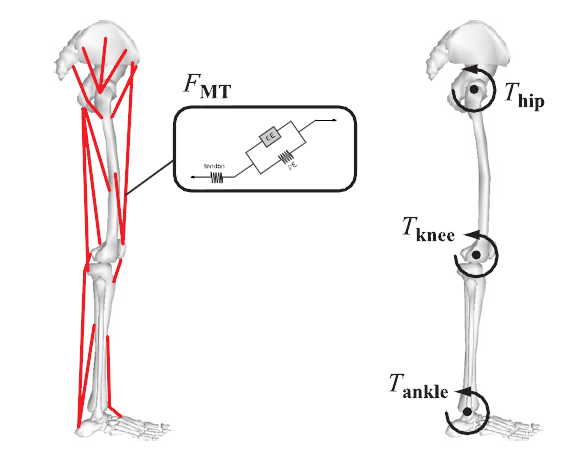
\includegraphics[width=.6\textwidth, height=.30\textheight]{musculoskeletal/fig/muscle-skeleton-torque.png}
    \caption{Συσχέτιση παραγόμενης δύναμης από τον μυ με ροπές στις αρθρώσεις\cite{erdemir07}}
    \label{fig:force-torques}
\end{figure}

\begin{equation}
    R_{ij} = - \frac{\partial L_{j}(q)}{\partial q_{i}}
    \label{equ:muscle-moment-arm}
\end{equation}

Είναι φανερό, ότι υπολογισμός της δύναμης που ασκεί ο μυς είναι απαραίτητη η γνώση της διάταξης την συγκεκριμένη χρονική στιγμή. Κάτι που πρέπει να τονίσουμε είναι ότι κάθε μυς έχει μια συγκεκριμένη γεωμετρία και τυλίγεται με διαφορετικό τρόπο πάνω στον σκελετό. Δεν μπορούμε να θεωρήσουμε ότι ένας μυς απλά ξεκινάει σε ένα σημείο Α και καταλήγει σε ένα άλλο σημείο Β. Είναι απαραίτητη η περιγραφή της διαδρομής που ακολουθεί από μια ακολουθία σημείων, αλλά και τον τρόπο με τον οποίο τυλίγεται στην διάταξη \cite{delp95}. Για να βρεθεί το μήκος του μυ αθροίζονται τα επιμέρους ευθύγραμμα τμήματα που τον δημιουργούν.




\chapter{Υλικά και Μέθοδοι}

Σε αυτή την ενότητα θα περιγράψουμε την διαδικασία με την οποία συλλέχθηκαν τα δεδομένα αλλά και την πορεία της επεξεργασίας τους ώστε να εξαχθούν τα επιθυμητά αποτελέσματα. Όπως φαίνεται στην εικόνα \ref{fig:methods-process1} αρχικά συλλέγονται τα δεδομένα με την βοήθεια της συσκευής \eng{Kinect}, αλλά και των εξωτερικών δυνάμεων αν είναι υπαρκτές. Τα δεδομένα αυτά προτού επεξεργαστούν στα μετέπειτα στάδια φιλτράρονται κατάλληλα ώστε να μειωθούν οι ανεπιθύμητες παρεμβολές του θορύβου. Έπειτα ακολουθεί η διαδικασία της αντίστροφης κινηματικές, που με την βοήθεια ενός μοντέλου εξάγονται οι γενικευμένες συντεταγμένες (γωνίες) στις αρθρώσεις. Με χρήση αριθμητικών μεθόδων παραγογίζουμε δύο φορές το αποτέλεσμα ώστε να έχουμε στην διάθεση μας τις γενικευμένες ταχύτητες και επιταχύνσεις των αρθρώσεων του μοντέλου. Εφαρμόζουμε αντίστροφη δυναμική και εξάγουμε τις γενικευμένες ροπές στις αρθρώσεις που απαιτούνται για να παράξουν την δοσμένη κίνηση. Τέλος, έχοντας προσδώσει τους κατάλληλους μύες στο μοντέλο με βάση την γεωμετρία, αλλά και της δυναμικής τους, μπορούν να εκτιμηθούν οι δυνάμεις που ασκεί ο κάθε μυς.

\begin{figure}[H]
    \centering
    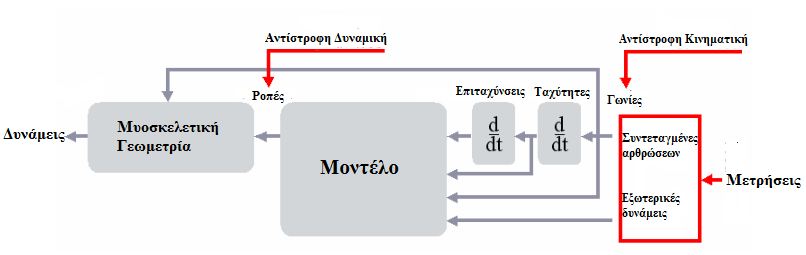
\includegraphics[width=1.0\textwidth]{methods/fig/process.png}
    \caption{Διαδικασία εξαγωγής των δυνάμενων\protect\footnotemark}
    \label{fig:methods-process1}
\end{figure}
\footnotetext{Εικόνα από την ιστοσελίδα \eng{\url{http://simtk-confluence.stanford.edu:8080/display/OpenSim/Overview+of+the+OpenSim+Workflow}}}

%%%%%%%%%%%%%%%%%%%%%%%%%%%%%%%%%%%%%%%%%%%%%%%%%%%%%%%%%%%%%%%%%%%%%%%%%%%%%%%%
\section{Καταγραφή της Κίνησης}

Όπως αναφέραμε χρησιμοποιούμε το \eng{Kinect} για την συλλογή των τροχιών των αρθρώσεων για μια δοσμένη κίνηση. Για την ανίχνευση του σκελετού εκμεταλλευόμαστε τον αλγόριθμο που είναι υλοποιημένος εσωτερικά στην συσκευή και έχουμε στην διάθεση μας στις τρισδιάστατες συντεταγμένες των αρθρώσεων. Το λογισμικό που χρησιμοποιείται για την καταγραφή της κίνησης έχει υλοποιηθεί στην \eng{C++} και βασίζεται στην βιβλιοθήκη της \eng{Microsoft} για το \eng{Kinect} (\eng{Microsoft Kinect SDK}). Επιπλέον, γίνεται χρήση φίλτρων για την εξομάλυνση του θορύβου και του τρέμουλο (\eng{jitter}). Τα αποτελέσματα μπορούν να καταγραφούν σε διαφορετικούς τύπους αρχείων, ώστε να χρησιμοποιηθούν στα μετέπειτα στάδια της ανάλυσης.

Το πρόγραμμα καταγραφής που υλοποιήθηκε έχει σαν στόχο την καταγραφή της χρονικής μεταβολής των θέσεων των αρθρώσεων και την βελτίωση των μετρήσεων. Για να ελαχιστοποιηθούν οι καθυστερήσεις και να μην ελαττωθεί ο ρυθμός επεξεργασίας των πακέτων που εισέρχονται από το \eng{Kinect}, έχουν ενεργοποιηθεί μόνο οι δυνατότητες παρακολούθησης του σκελετού και την πρόσληψη έγχρωμου βίντεο, για να μπορούμε να αντιληφθούμε το ορατό πεδίο του αισθητήρα όπως φαίνεται στην εικόνα \ref{fig:motion-capture}.

\begin{figure}[H]
    \centering
    \includegraphics[width=.9\textwidth]{methods/fig/motion-capture.png}
    \caption{Επίδειξη του συστήματος καταγραφής της κίνησης που υλοποιήθηκε}
    \label{fig:motion-capture}
\end{figure}

Πρέπει να σημειωθεί ότι η υλοποίηση έγινε με χρήση της βιβλιοθήκη \eng{OpenGL}. Υπάρχουν δύο παράθυρα, όπου στο ένα αναπαριστάται η τελευταία ακολουθία θέσεων του σκελετού, ενώ στο άλλο γίνεται αποτύπωση της έγχρωμης εικόνας που λαμβάνουμε ανά τακτικά χρονικά διαστήματα σαν εικόνα υφής, με αποτέλεσμα να έχουμε μια ανανέωση του περιεχομένου (δηλαδή βίντεο). Η περιήγηση στο τρισδιάστατο χώρο του αριστερού παραθύρου μπορεί να γίνει με την βοήθεια του ποντικιού και του πληκτρολογίου, δίνοντας την δυνατότητα αναπαράστασης του μοντέλου από διαφορετικές οπτικές γωνίες.

Εσωτερικά αποθηκεύονται οι παρελθοντικές τιμές των θέσεων σε ειδικές δομές μαζί με όλη την πληροφορία που διαθέτει το \eng{Kinect}. Παρέχεται η δυνατότητα αποθήκευσης των δεδομένων σε δυαδική, μορφή η οποία είναι εύκολη στην ανάγνωση και δεν απαιτεί υλοποίηση πολύπλοκων συναρτήσεων ανάγνωσης. Επίσης υπάρχουν επιλογές για αποθήκευση των τροχιών σε μορφή \lq \eng{.dat}\rq\; της \eng{Matlab} και σε μορφή \lq \eng{.trc}\rq  , που είναι συμβατή με το εργαλείο \eng{OpenSim}.

%%%%%%%%%%%%%%%%%%%%%%%%%%%%%%%%%%%%%%%%%%%%%%%%%%%%%%%%%%%%%%%%%%%%%%%%%%%%%%%%
\section{Δημιουργία του Μοντέλου}

Πριν περιγράψουμε την διαδικασία της δημιουργίας του μοντέλου θα ήθελα να αναφερθώ στα εργαλεία που χρησιμοποιήθηκαν. Για την μοντελοποίηση αλλά και την διεξαγωγή των αναλύσεων χρησιμοποιήθηκε το ανοιχτό εργαλείο-βιβλιοθήκη \eng{OpenSim}. Το \eng{OpenSim} είναι μια πλατφόρμα που βασίζεται στην μηχανή \eng{SimTK Simbody} για την μοντελοποίηση, προσομοίωση και ανάλυση νευρομυοσκελετικών συστημάτων \cite{delp07}. Το εργαλείο διαθέτει γραφική διεπαφή, αλλά και διεπαφή για τον προγραμματιστή σε γλώσσα \eng{C++}. Είναι δυνατή η επέκταση του λογισμικού με την βοήθεια \eng{plugins}. Το \eng{OpenSim} χρησιμοποιείται ευρέως από την επιστημονική κοινότητα κυρίως σε βιοϊατρικές εφαρμογές. Η κοινότητα διαθέτει μεγάλο αριθμό από έτοιμα μοντέλα, πειραματικά δεδομένα και επιπρόσθετα εργαλεία για την διεξαγωγή των αναλύσεων.

\begin{figure}[H]
    \centering
    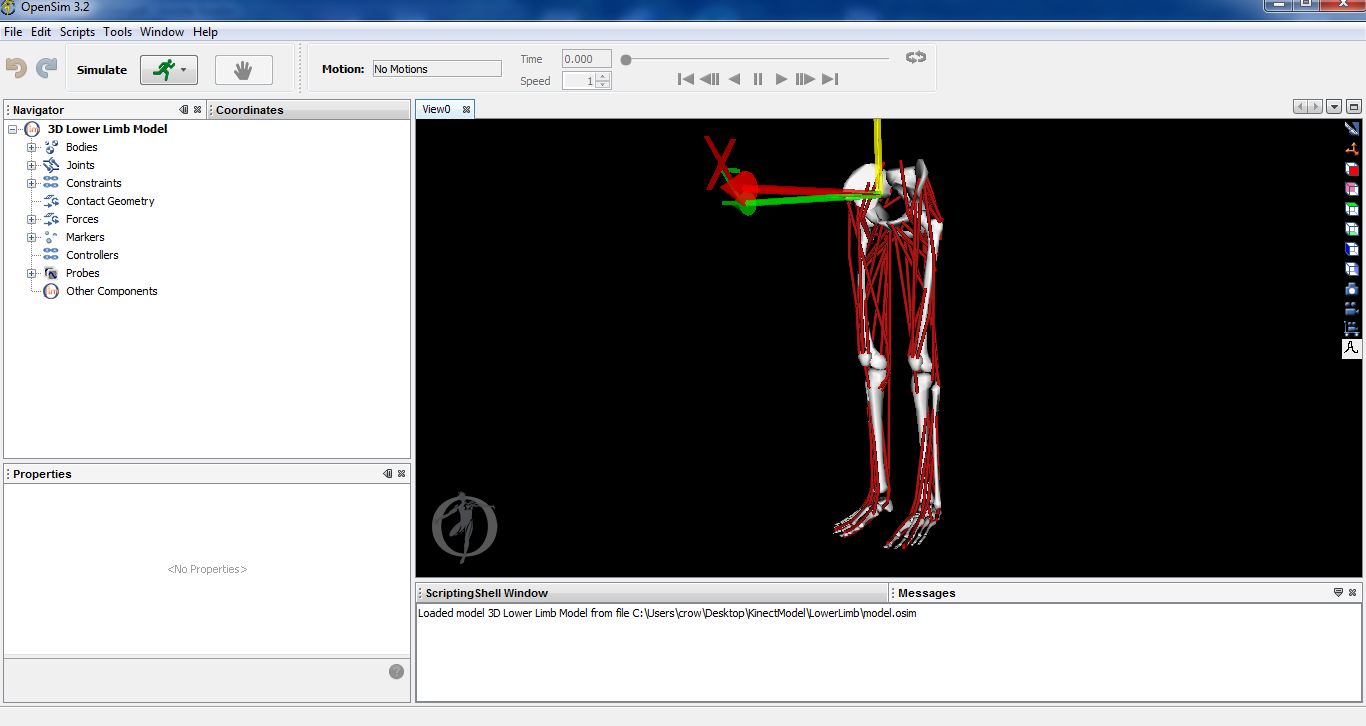
\includegraphics[width=0.8\textwidth]{methods/fig/opensim.png}
    \caption{Γραφική διεπαφή του \eng{OpenSim}}
    \label{fig:opensim-gui}
\end{figure}

Δεν θα μπορούσα να παραλείψω βέβαια και το \eng{Simbody}, το οποίο είναι η καρδιά της πλατφόρμας. Σαν μηχανή φυσικής, δίνει την δυνατότητα περιγραφής πολύπλοκων διατάξεων με έναν μεγάλο αριθμό από έτοιμα στοιχεία όπως είναι η μοντελοποίηση δυνάμενων, εισαγωγή περιορισμών στην κίνηση, περιγραφή της διάταξης, ποικίλα τύπων βαθμών ελευθερίας και άλλα πολλά. Έχει σχεδιαστεί κατάλληλα ώστε να ωθεί την αποδοτικότητα και παράλληλα να μην μειώνει την ευελιξία. Είναι ένα εργαλείο που σου δίνει την δυνατότητα να περιγράφεις και να προσομοιώσεις τα φαινόμενα που μελετάς.

Όσον αφορά τις δυνατότητες που προσφέρει η προγραμματιστική βιβλιοθήκη του \eng{OpenSim} μπορούμε να διακρίνουμε κάποια βασικά χαρακτηριστικά \ref{fig:opensim-architecture}. Βλέπουμε ότι στην βάση βρίσκεται το \eng{Simbody}. Επιπλέον, έχει δοθεί η δυνατότητα περιγραφής του μοντέλου και επιπρόσθετα στοιχεία που βοηθούν στο να γίνει η ανάλυση. Το \eng{OpenSim} βοηθάει στο να γίνει η περιγραφής της σκελετικής διάταξης, να προδοθούν βαθμοί ελευθερίας και περιορισμοί στην κίνηση. Ακόμη υπάρχει η δυνατότητα μοντελοποίησης των μυών και η προσθήκη τους στην διάταξη. Όπως θα δούμε και στην συνέχει μπορούν να εξαχθούν πληθώρα είδη αναλύσεων, που μπορούν να χρησιμοποιηθούν ακόμη και σε ιατρικές εφαρμογές, αλλά και όχι μόνο.

\begin{figure}[H]
    \centering
    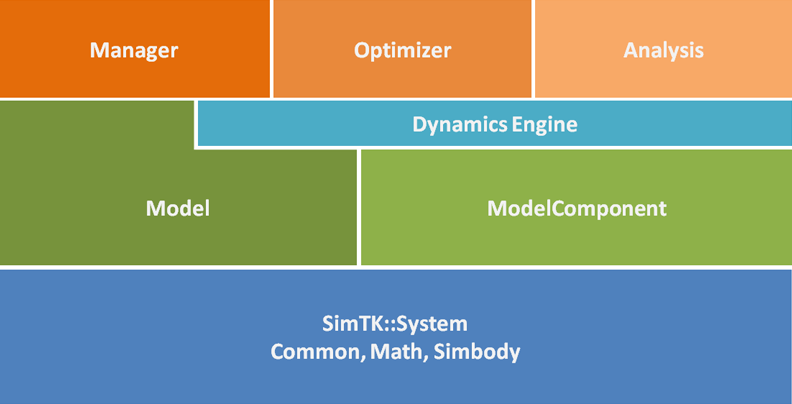
\includegraphics[width=0.8\textwidth]{methods/fig/opensim-architecture.png}
    \caption{Συνοπτική αρχιτεκτονική της βιβλιοθήκης του \eng{OpenSim}\protect\footnotemark}
    \label{fig:opensim-architecture}
\end{figure}
\footnotetext{Εικόνα από την ιστοσελίδα \eng{\url{http://simtk-confluence.stanford.edu:8080/display/OpenSim/The+OpenSim+API}}}


%%%%%%%%%%%%%%%%%%%%%%%%%%%%%%%%%%%%%%%%%%%%%%%%%%%%%%%%%%%%%%%%%%%%%%%%%%%%%%%%
\subsection{Επεξήγηση του Μοντέλου}

Για την διεξαγωγή των προσομοιώσεων είναι αναγκαία η σχεδίαση ενός μοντέλου που θα είναι όσο το δυνατών πιο αντιπροσωπευτικό σε σχέση με το πραγματικό. Η διαδικασία είναι πολύπλοκη και απαιτεί γνώσεις όχι της μόνο φυσιολογίας του ανθρώπου, αλλά και γνώσεις ώστε να περιγραφεί η λειτουργία του μοντέλου. Στην παρούσα μελέτη έχει μοντελοποιηθεί το τμήμα των κάτω άκρα του ανθρώπου, ώστε να γίνει η μελέτη κατά την διεξαγωγή κινήσεων.

Το μοντέλο αποτελείται από 20 βαθμούς ελευθερίας, από τους οποίους οι 6 έχουν να κάνουν με τον προσανατολισμού και την περιστροφή της λεκάνης, που είναι και η ρίζα της ιεραρχίας. Οπότε έχουμε άλλους 7 βαθμούς ελευθερίας για κάθε πόδι. Επίσης το μοντέλο διαθέτει 43 μύες για κάθε πόδι οι οποίοι είναι τοποθετημένοι με βάση την πραγματική τους γεωμετρία γύρω από τα οστά. Οι μύες είναι σε θέσει να παράξουν έργο στις καθαρισμένες αρθρώσεις ώστε να παραχθεί η επιθυμητή κίνηση. Επίσης, λόγο της έλλειψης δεδομένων που αφορούν τις εξωτερικές δυνάμεις αντίδρασης από το δάπεδο κατά την κίνηση έχει γίνει η κατάλληλη μοντελοποίηση τους με χρήση δυνάμεων επαφής. Το μοντέλο έχει δημιουργηθεί στα πλαίσια μελέτης πως μπορεί μια εγχείρηση να αλλάξει τις παραμέτρους των μυών και κατά συνέπεια το αποτέλεσμα της βάδισης με βάση το \cite{delp90} και τροποποιήθηκε κατάλληλα στην παρούσα εργασία.

\begin{figure}[H]
    \centering
    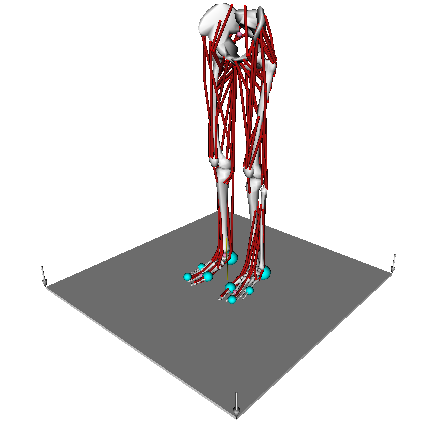
\includegraphics[height=0.38\textheight]{methods/fig/lower-limb-model.png}
    \caption{Μυοσκελετικό μοντέλο μαζί και δάπεδο αντίδρασης}
    \label{fig:lower-limb-model}
\end{figure}

\begin{center}
    \begin{tabular}{ccc}
        \toprule
        % after \\: \hline or \cline{col1-col2} \cline{col3-col4} ...
        Άρθρωση & Κάτω όριο & Πάνω όριο\\
        \midrule
        \eng{pelvis\_till (z)} & $-90^{o}$ & $+90^{o}$\\
        \eng{pelvis\_list (x)} & $-90^{o}$ & $+90^{o}$\\
        \eng{pelvis\_rotation (y)} & $-90^{o}$ & $+90^{o}$\\
        \eng{pelvis\_tx} & $-5$ & $+5$\\
        \eng{pelvis\_ty} & $-1$ & $+2$\\
        \eng{pelvis\_tz} & $-3$ & $+3$\\
        \eng{hip\_flexion} & $-95^{o}$ & $+95^{o}$\\
        \eng{hip\_adduction} & $-50^{o}$ & $+15^{o}$\\
        \eng{hip\_rotation} & $-20^{o}$ & $+20^{o}$\\
        \eng{knee\_angle} & $-120^{o}$ & $+0^{o}$\\
        \eng{ankle\_angle} & $-30^{o}$ & $+30^{o}$\\
        \eng{subtalar\_angle} & $-20^{o}$ & $+20^{o}$\\
        \eng{mtp\_angle} & $-30^{o}$ & $+30^{o}$\\
        \bottomrule
    \end{tabular}
    \captionof{table}{Βαθμοί ελευθερίας με τους αντίστοιχους περιορισμούς}
    \label{tab:model-dof}
\end{center}

Όπως φαίνεται και στον πίνακα \ref{tab:model-dof} παρουσιάζονται οι βαθμοί ελευθερίας του μοντέλου μαζί με τους περιορισμούς στην επιτρεπτή κίνηση. Ο γοφός έχει τρις περιστροφικούς βαθμούς, το γόνατο έναν, ο αστράγαλος δύο και τα δάχτυλα των ποδιών έναν. Η λεκάνη φροντίζει να προσανατολίσει και να τοποθετήσει κατάλληλα το μοντέλο στο χώρο και στην πραγματικότητα δεν παίζει κάποιο ρόλο στην κίνηση. Αυτός ο πλεονασμός της λεκάνη είναι μια από της τροποποιήσεις του αρχικού μοντέλου ώστε να μπορεί να βρεθεί το κάτω τμήμα σε διαφορετικές διατάξεις στον χώρο.

Η έλλειψη εξωτερικών δυνάμεων αντίδρασης από το δάπεδο είναι σοβαρό μειονέκτημα που οδηγεί σε προσεγγίσεις της πραγματικότητας. Αναγκαστικά υιοθετήθηκαν τεχνικές εκτίμησης των δυνάμεων με μοντελοποίηση της επαφής με το δάπεδο \cite{seitha11}. Το \eng{OpenSim} χρησιμοποιεί δύο τύπων δυνάμεων επαφής που έχουν υλοποιηθεί από το \eng{Simbody}. Η πρώτη είναι η \eng{Hunt Crossley Force} που βασίζεται στην θεωρία επαφής του \eng{Hertz} \cite{hunt75}. Αυτή η μέθοδος υπολογίζει την ελαστική παραμόρφωση αναλυτικά και το \eng{Simbody} υποστηρίζει κάποια βασικά γεωμετρικά σχήματα. Στην μοντελοποίηση που κάναμε έχει χρησιμοποιηθεί μια επιφάνεια για το δάπεδο και έχουν τοποθετηθεί σφαίρες στις πατούσες. Η εναλλακτική λύση είναι η αναπαράσταση της γεωμετρίας με πλέγματα (\eng{mesh}) τα οποία αποτελούνται από ελατήρια για την μοντελοποίηση της ελαστικότητας \cite{hertz82}.

\begin{figure}[H]
    \centering
    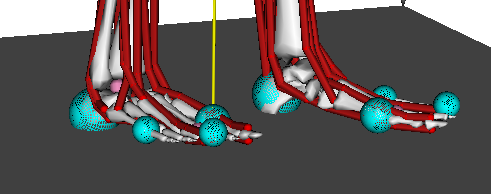
\includegraphics[width=0.8\textwidth]{methods/fig/foot-contact.png}
    \caption{Εποπτική αναπαράσταση των σφαιρών αντίδρασης στα πόδια}
    \label{fig:foot-contact}
\end{figure}

Όσον αφορά τους μύες, έχουν τροποποιηθεί ώστε να χρησιμοποιούν το έτοιμο μοντέλο μυ \eng{Millard2013EquilibriumMuscle} που είναι υλοποιημένο στην βιβλιοθήκη του \eng{OpenSim}. Οι παράμετροι των μυών (μέγιστη παραγόμενη δύναμη, βέλτιστο μήκος μυ, μήκος χαλαρότητας του τένοντα, σχετική γωνία μεταξύ μυ και τένοντα, γεωμετρία) έχουν προσδιοριστεί από το αρχικό μοντέλο και είναι συμβατά με το νέο μοντέλο μυ.

%%%%%%%%%%%%%%%%%%%%%%%%%%%%%%%%%%%%%%%%%%%%%%%%%%%%%%%%%%%%%%%%%%%%%%%%%%%%%%%%
\section{Προετοιμασία για την Αντίστροφη Κινηματική}

Αφού έχει καταγραφεί μια κίνηση και υπάρχει το αντίστοιχο μοντέλο μπορεί να λυθεί το πρόβλημα της αντίστροφης κινηματικής ώστε να προσδιορισθούν οι γενικευμένες συντεταγμένες (συνήθως γωνίες) για την δοσμένη κίνηση. Προτού όμως εκτελέσουμε την αντίστροφη κινηματική πρέπει να γίνουν κάποια επιπλέον βήματα.

%%%%%%%%%%%%%%%%%%%%%%%%%%%%%%%%%%%%%%%%%%%%%%%%%%%%%%%%%%%%%%%%%%%%%%%%%%%%%%%%
\subsection{Τοποθέτηση Ενδείξεων}

Αρχικά πρέπει να προσδιοριστούν αντιστοιχίες μεταξύ της καταγεγραμμένης κίνησης και του μοντέλου. Ωστόσο μην ξεχνάμε ότι το πρόβλημα της αντίστροφης κινηματικής προσπαθεί να βρει τις γωνίες που πρέπει να τροφοδοτήσει το μοντέλο ώστε να ταιριάξει με την δοσμένη διάταξη της κίνησης. Αφού τα πειράματα έγινα με την βοήθεια του \eng{Kinect}, έχουμε στην διάθεση μας τις θέσεις των αρθρώσεων. Συνεπώς, πρέπει να τοποθετηθούν οι αντίστοιχες ενδείξεις και στο μοντέλο.

\begin{figure}[H]
    \centering
    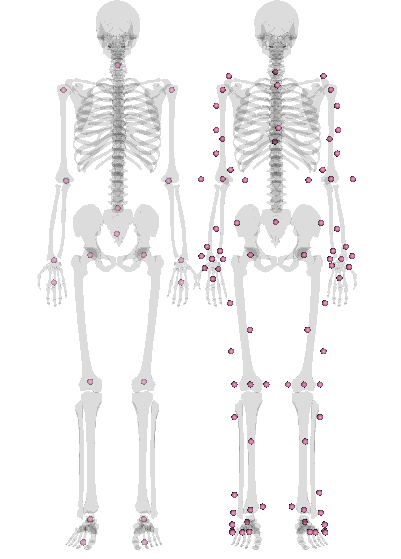
\includegraphics[height=0.6\textheight]{methods/fig/kinect-vicon-markers.png}
    \caption{Σύγκριση συστήματος ενδείξεων του \eng{Kinect} και του \eng{Vicon} δεξιά}
    \label{fig:kinect-vicon-markers}
\end{figure}

Στην εικόνα \ref{fig:kinect-vicon-markers} με ροζ χρώμα συμβολίζεται οι ενδείξεις (\eng{marker}). Από αριστερά βλέπουμε τις ενδείξεις που απαιτούνται για να συνδεθεί η καταγεγραμμένη κίνηση από το \eng{Kinect}, ενώ από δεξιά βλέπουμε τους δείκτες που απαιτούνται για να γίνει μια καταγραφή από ένα επαγγελματικό σύστημα της εταιρίας \eng{Vicon}. Οι ενδείξεις προσδιορίζονται με βάση την εφαρμογή, ωστόσο λόγο ότι ο προσανατολισμός και η θέση στο χώρο ενός τμήματος του σώματος, όπως είναι τα οστά, απαιτεί ώστε να βρεθεί μοναδική λύση τουλάχιστον τρία μη συνευθειακά σημεία σε κάθε τμήμα. Αυτός είναι και ο λόγος για τον οποίον ο δεξής σκελετός έχει πιο πολλές ενδείξεις. Αυτό είναι και ένα βασικό μειονέκτημα του συστήματος μας σε σχέση με επαγγελματικά συστήματα, δηλαδή για κάποιες κινήσεις μπορεί να μην βρεθεί ο σωστός προσανατολισμός. Ωστόσο για απλές κινήσεις το αποτέλεσμα της αντίστροφης κινηματικής δίνει ικανοποιητικά αποτελέσματα για την διάταξη μας, αν συγκρίνουμε και το αντίστοιχο κόστος το να έχει κανείς ένα επαγγελματικό σύστημα.

%%%%%%%%%%%%%%%%%%%%%%%%%%%%%%%%%%%%%%%%%%%%%%%%%%%%%%%%%%%%%%%%%%%%%%%%%%%%%%%%
\subsection{Κανονικοποίησης του Μοντέλου}

Το τελευταίο πράγμα που πρέπει να γίνει είναι η κανονικοποίησης του γενικού μοντέλου που έχουμε στην διάθεση μας, ώστε να αρμόζει σε διαφορετικά σωματότυπα. Το \eng{OpenSim} διαθέτει δυνατότητα μετατροπής του μοντέλου αλλά και την θέση των ενδείξεων από το γενικό στο ειδικό μοντέλο. Η διαδικασία είναι σχετικά απλή και βελτιώνει σημαντικά το αθροιστικό σφάλμα της αντίστροφης κινηματικής. Με βάση τις ενδείξεις που έχουν τοποθετηθεί στο γενικό μοντέλο γίνεται μια δημιουργία ζευγαριών που αντιπροσωπευθούν κάποιο τμήμα του σώματος (π.χ. η ένδειξη του γοφού και του γονάτου αντιστοιχεί στο μηριαίο οστό) και θα ληφθούν υπόψη ώστε να γίνει ομαλή μεταβολή του τμήματος, για να ταιριάξει στις μετρήσεις.

Έχει γίνει κατάλληλη επιλογή των τμημάτων και των ζευγαριών ενδείξεων ώστε να μεταβληθούν κατάλληλα όλα τα τμήματα του σώματος. Επίσης δίνεται η δυνατότητα να διατηρηθεί η μάζα του γενικού μοντέλου. Το γενικό μοντέλο αντιπροσωπευθεί άντρα ύψους 1.80\eng{cm} και ζυγίζει 75\eng{kg}. Το κάτω τμήμα που έχει παρθεί ζυγίζει 41\eng{kg}. Η μάζα και η αδράνεια κάθε οστού έχει προσδιοριστεί για το γενικό μοντέλο και τροποποιείται ανάλογα με βάση τις μετρήσεις.

\begin{center}
    \begin{tabular}{ccc}
        \toprule
        Τμήμα του σώματος & 1η ένδειξη & 2η ένδειξη\\
        \midrule
        \eng{pelvis} & \eng{HIP\_RIGHT} & \eng{HIP\_LEFT}\\
        \eng{femru} & \eng{HIP} & \eng{KNEE}\\
        \eng{tibia} & \eng{KNEE} & \eng{ANKLE}\\
        \eng{calcn} & \eng{ANKLE} & \eng{FOOT}\\
        \bottomrule
    \end{tabular}
    \captionof{table}{Τμήματα του σώματος και τα ζευγάρια των ενδείξεων για τα κάτω άκρα}
    \label{tab:scale-pairs}
\end{center}

%%%%%%%%%%%%%%%%%%%%%%%%%%%%%%%%%%%%%%%%%%%%%%%%%%%%%%%%%%%%%%%%%%%%%%%%%%%%%%%%
\subsection{Διεξαγωγή της Αντίστροφης Κινηματικής}

Αφού έχουν γίνει τα παραπάνω πλέων μπορεί να εκτελεστεί η αντίστροφη κινηματική και να παραχθούν οι γωνίες που απαιτούνται για την παραγωγή της δοσμένης κίνησης από το μοντέλο. Το αποτέλεσμα την αντίστροφης κινηματικής είναι ζωτικής σημασίας για τα μετέπειτα στάδια της ανάλυσης. Οι υπολογισμένες γωνίες αν αναπαρασταθούν δεν θα πρέπει να έχουν απότομες μεταβολές από μια στιγμή σε άλλη, ώστε να μην παράγουν μη φυσιολογικές επιταχύνσεις και με αποτέλεσμα δυνάμεις. Κατά την εύρεση λύσεων υπάρχουν γωνίες για τις οποίες η διάταξη βρίσκεται σε απροσδιοριστία μορφή. Το τελευταίο μπορεί να αποφευχθεί αν εισαχθούν οι κατάλληλοι περιορισμοί στις κινήσεις της διάταξης αφότου έχει μελετηθεί εκ των προτέρων.

Κατά την διεξαγωγή της αντίστροφης κινηματικής μαζί με το κανονικοποιημένο μοντέλο τροφοδοτούμε και τις συντεταγμένες που έχουμε καταγράψει από το \eng{Kinect}, οι οποίες βρίσκονται σε κατάλληλη μορφή (*.\eng{trc}) που υποστηρίζεται από το \eng{OpenSim}.

%%%%%%%%%%%%%%%%%%%%%%%%%%%%%%%%%%%%%%%%%%%%%%%%%%%%%%%%%%%%%%%%%%%%%%%%%%%%%%%%
\section{Προσδιορισμός Δυνάμενων και Διεγέρσεων Μυών}

Αφού έχουμε στην διάθεση μας τα αποτελέσματα της αντίστροφης κινηματικής το επόμενο βήμα είναι ο προσδιορισμός των γενικευμένων ροπών στις αρθρώσεις του μοντέλου, αλλά και η εκτίμηση των δυνάμεων που συνεισφέρει ο κάθε μυς. Ας υπενθυμίσουμε την σχέση που περιγράψαμε \ref{equ:dynamics-equation}, η οποία αποτελεί την λύση του προβλήματος του προσδιορισμού των ροπών στις αρθρώσεις. Η διαδικασία ονομάζεται αντίστροφη δυναμική (\eng{inverse dynamics}). Τα απαραίτητα στοιχεί είναι οι εξωτερικές δυνάμεις, το αποτέλεσμα από την αντίστροφη κινηματική, οι ταχύτητες και οι επιταχύνσεις.

Αν θέλαμε να υπολογίσουμε τις δυνάμεις των μυών πρέπει να συνδυάσουμε διαφορετικές τεχνικές που βασίζονται στην θεωρία της βελτιστοποίησης, αφού για μια δοσμένη κίνηση υπάρχουν πολλές λύσεις (δυνάμεις μυών) που μπορούν να παράξουν την κίνηση. Για το λόγο αυτό στην ανάλυση μπαίνουν κάποια κριτήρια που θα περιορίσουν τις επιτρεπτές λύσεις και θα παράξουν μια βέλτιστη με βάση αυτών. Στην βιβλιογραφία αυτή η τεχνική αποκαλείται στατική βελτιστοποίηση (\eng{static optimization}).

Ένα βήμα πιο πέρα στην ανάλυση είναι, αφού έχουν προσδιοριστεί οι δυνάμεις που ασκεί κάθε μυς κάθε χρονική στιγμή να βρεθεί η απαραίτητη διέγερση που πρέπει να τροφοδοτηθεί στον μυ ώστε να παράξει την απαιτούμενη δύναμη. Με αυτή την διαδικασία πλέων μπορούμε να φτάσουμε σε επίπεδο νευρικών διεγέρσεων και να ελέγχουμε την κίνηση από αυτές. Η μέθοδος που προσδιορίζει τις διεγέρσεις αποκαλείται υπολογισμός των μυϊκών διεγέρσεων (\eng{computed muscle control}).

Μια τυπική ροή ώστε να φτάσουμε σε νευρικό επίπεδο διεγέρσεων περιγράφεται από την εικόνα \ref{fig:ik-to-excitation}. Η διεργασία πριν τον υπολογισμό των μυϊκών διεγέρσεων ονομάζεται αλγόριθμος υπολειμματικής μείωσης (\eng{residual redaction algorithm}) και μπορεί να παραληφθεί, αλλά γενικά βελτιώνει το αποτέλεσμα.

\begin{figure}[H]
    \centering
    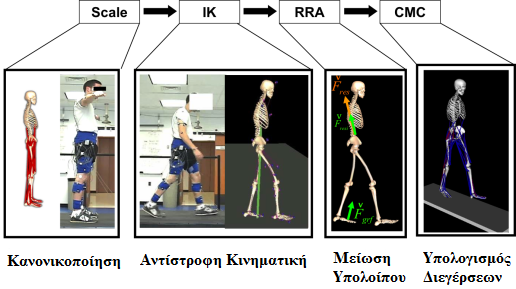
\includegraphics[width=0.8\textwidth]{methods/fig/ik-to-excitation.png}
    \caption{Τυπική ροή υπολογισμού των μυϊκών διεγέρσεων\protect\footnotemark}
    \label{fig:ik-to-excitation}
\end{figure}
\footnotetext{Εικόνα από την ιστοσελίδα \eng{\url{http://simtk-confluence.stanford.edu:8080/display/OpenSim/Overview+of+the+OpenSim+Workflow}}}

%%%%%%%%%%%%%%%%%%%%%%%%%%%%%%%%%%%%%%%%%%%%%%%%%%%%%%%%%%%%%%%%%%%%%%%%%%%%%%%%
\subsection{Εκτίμηση των Μυϊκών Δυνάμεων}

Όπως αναφέραμε η διαδικασία προσδιορισμού των μυϊκών δυνάμεων βασίζεται στην βελτιστοποίηση. Ξέρουμε για κάθε άρθρωση την χρονική ακολουθία των ροπών από την αντίστροφη δυναμική. Επίσης ξέρουμε από την γεωμετρία του μοντέλου την τοποθεσία κάθε μυ και σε ποια άρθρωση συνεισφέρει έργο. Σε μια άρθρωση μπορούν να συνεισφέρουν έργο παραπάνω από ένας μύες. Ένα κριτήριο βελτιστοποίησης μπορεί να είναι το να ελαχιστοποιηθεί η ενέργεια ώστε να παραχθεί η δοσμένη κίνηση. Το κριτήριο αυτό, ανάλογα και την εφαρμογή, είναι λογικό αφού για κάθε κίνηση προσπαθούμε να καταβάλουμε όσον το δυνατών λιγότερη προσπάθεια στην πράξη, όταν βέβαια δεν υπάρχει κάποια σοβαρή ασθένεια. Συμπερασματικά το πρόβλημα μπορεί να διατυπωθεί μαθηματικά ως εξής.

\begin{equation}
    \begin{gathered}
        \underset{q_{j}}{\text{\eng{minimize}}} \sum_{i=1}^{N} a_{i}^{p} \\
        \text{\eng{s.t.}} \quad
        \sum_{i=1}^{N} (a_{i} \cdot f(f^{o}_{i}, l_{i}, v_{i})) \cdot  R_{ij} = \tau_{j}, \quad \forall j
    \end{gathered}
    \label{equ:static-optimization}
\end{equation}

Όπου $a_i$ είναι το επίπεδο ενεργοποίησης του μυ $i$, η συνάρτηση $f(f^{o}_{i}, l_{i}, v_{i})$ είναι η δύναμη που παράγει ο μυς χωρίς να λάβουμε υπόψη τον τένοντα με $f^{o}_{i}, l_{i}, v_{i}$ να είναι ή μέγιστη ισομετρική δύναμη, το μήκος και τη ταχύτητα του μυ αντίστοιχα. Το $R_{ij}$ είναι η μυϊκή ροπή αδράνειας και το $\tau_{j}$ είναι η ροπή στην άρθρωση $j$.

%%%%%%%%%%%%%%%%%%%%%%%%%%%%%%%%%%%%%%%%%%%%%%%%%%%%%%%%%%%%%%%%%%%%%%%%%%%%%%%%
\subsection{Προσδιορισμός των Μυϊκών Διεγέρσεων}

Η διαδικασία προσδιορισμού των διεγέρσεων είναι σχετικά πολύπλοκη και συνδυάζει πολλές μεθόδους μαζί και για διευκόλυνση θα περιγράψουμε την διαδικασία ιεραρχικά. Η διαδικασία παίρνει σαν ορίσματα τις πειραματικές τροχαίες των αρθρώσεων, μαζί μαι τις δύο πρώτες παραγώγους και τις εξωτερικές δυνάμεις. Το αποτέλεσμα είναι οι διεγέρσεις για κάθε μυ σε κάθε χρονική στιγμή.

Όπως περιγράφεται και στην εικόνα \ref{fig:cmc-diagram}, βλέπουμε ότι όλη η διαδικασία είναι κλειστού βρόγχους, που σημαίνει ότι κάθε στιγμή το σύστημα τροφοδοτείται κατάλληλα ώστε η παραγόμενη κίνηση να είναι όσο το δυνατών ταυτόσημη με την πειραματική. Χρησιμοποιείται \eng{PD} ελεγκτής και οι σταθερές επιλέγονται ώστε να πετύχουμε κρίσιμη απόσβεση ($\overrightarrow{k}_v = 2 \cdot \sqrt{\overrightarrow{h}_p}$). Επίσης βλέπουμε ότι η επιθυμητή επιτάχυνσή $\ddot{\overrightarrow{q}}^{*}$ υπολογίζεται για μελλοντική τιμή $t + \tau $. Αυτό γιατί οι μύες έχουν μια καθυστέρηση, οπότε η διέγερση θα πρέπει να προηγείται κατά μια μικρή χρονική στιγμή (συνήθως $\tau = 0.01$. Έπειτα εκτελείται στατική βελτιστοποίηση για να υπολογιστούν οι απαιτούμενες διεγέρσεις που στην συνέχει τροφοδοτούνται στον σύστημα με την βοήθεια της ορθής δυναμικής, η οποία θα παράξει την κίνηση με βάση αυτών.

\begin{figure}[H]
    \centering
    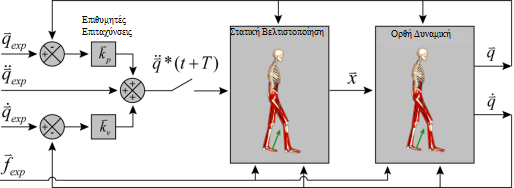
\includegraphics[width=0.8\textwidth]{methods/fig/cmc-diagram.png}
    \caption{Διάγραμμα της διαδικασίας υπολογισμού μυϊκών διεγέρσεων\cite{thelen06}}
    \label{fig:cmc-diagram}
\end{figure}

Η διαδικασία είναι σύνθετη και στην πράξει έχει μεγάλες καθυστερήσεις, που ανάλογα από τον υπολογιστή μπορεί να κυμαίνονται από 15 λεπτά για έναν σύγχρονο υπολογιστή έως και πάνω από μισή ώρα για πιο παλιούς ώστε να παραχθεί ένα αποτέλεσμα διάρκειας μισού λεπτού. Επίσης η διαδικασία μπορεί να διακοπεί αν δεν πληρούνται τα επιτρεπτά όρια ανοχής σε σφάλματα. Συχνά για την βελτίωση της διαδικασίας εισάγονται επιπλέον εφεδρικοί κινητήρες στις αρθρώσεις για να παρέχουν την απαραίτητη ροπή ώστε να παραχθεί η κίνηση, καθώς οι μύες μπορεί να μην είναι σε θέση να οδηγήσουν το σύστημα στην επιθυμητή κατάσταση. Το τελευταίο οφείλεται συνήθως σε απλοποιήσεις στο μοντέλο, μειώνοντας τους μύες με αποτέλεσμα να μην επαρκεί η κινητική τους δύναμη. Επειδή συνήθως δεν μπορούν να αποφευχθούν οι εφεδρικοί κινητήρες, αν δούμε ότι η προσομοίωση τρέχει ήμαστε σε θέση να ελαττώσουμε την επιρροή τους και να βασιστούμε στους μύες του μοντέλου.

%%%%%%%%%%%%%%%%%%%%%%%%%%%%%%%%%%%%%%%%%%%%%%%%%%%%%%%%%%%%%%%%%%%%%%%%%%%%%%%%
\section{Ορθή Δυναμική}

Η προσέγγιση της μελέτης της ανθρώπινης κίνησης με την βοήθεια της ορθή δυναμική έχει σαν στόχο την επαλήθευση των αποτελεσμάτων από τις προηγούμενες διαδικασίες, αλλά και δίνεται η δυνατότητα μελέτης της απόκρισης του μοντέλου σε μεταβολές των παραμέτρων. Στην παρούσα εργασία απλά επαληθεύουμε το αποτέλεσμα των μυϊκών διεγέρσεων που υπολογίστηκαν, είναι σε θέση να παράξει ταυτόσημη κίνηση με αυτή που καταγράφτηκε. Το τελευταίο είναι γενικά ένα δύσκολο πρόβλημα και συνήθως το αποτέλεσμα φεύγει στην αστάθεια μετά από ένα μικρό χρονικό διάστημα, αφού συσσωρεύονται σφάλματα κατά τις προηγούμενες διαδικασίες.

\begin{figure}[H]
    \centering
    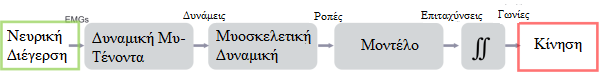
\includegraphics[width=0.8\textwidth]{methods/fig/forward-simulation.png}
    \caption{Στάδια της παραγωγής κίνηση με ορθή δυναμική\protect\footnotemark}
    \label{fig:forward-simulation}
\end{figure}
\footnotetext{Εικόνα από την ιστοσελίδα \eng{\url{http://simtk-confluence.stanford.edu:8080/display/OpenSim/Overview+of+the+OpenSim+Workflow}}}

Όπως φαίνεται και στην εικόνα \ref{fig:forward-simulation} η διαδικασία ξεκινά με τις νευρικές διεγέρσεις. Στην συνέχει με βάση κάποιου μοντέλου ενός μυ υπολογίζεται η δύναμη που παράγει. Κατόπιν οι μυϊκές δυνάμεις μετατρέπονται σε ροπές με βάση την γεωμετρία, την τοποθεσία και την διάταξη στην οποία βρίσκεται το μοντέλο, αφού η παραγωγή δύναμης από τον μυ εξαρτάται από αρκετούς παράγοντες. Τέλος με βάση την δομή του μοντέλου και την εξίσωση \ref{equ:forward-dynamics} υπολογίζονται οι επιταχύνσεις που στην συνέχει ολοκληρώνονται και παράγουν τις γενικευμένες γωνίες, που με την σειρά τους δημιουργούν την κίνηση.

Η διαδικασία είναι σχετικά ευθείς και απλή, αλλά κρύβει πολλά προβλήματα, ιδιαίτερα σε πολύπλοκες διατάξεις όπως είναι το ανθρώπινο σώμα. Άλλωστε αυτός ήταν και ο λόγος για την δημιουργία πολύπλοκων μεθόδων υπολογισμού των μυϊκών διεγέρσεων (μέθοδος υπολογισμού μυϊκών διεγέρσεων) ώστε να μειωθούν τα σφάλματα και να παραχθεί μια ικανοποιητική κίνηση.


%%%%%%%%%%%%%%%%%%%%%%%%%%%%%%%%%%%%%%%%%%%%%%%%%%%%%%%%%%%%%%%%%%%%%%%%%%%%%%%%%
\chapter{Αποτελέσματα}

%%%%%%%%%%%%%%%%%%%%%%%%%%%%%%%%%%%%%%%%%%%%%%%%%%%%%%%%%%%%%%%%%%%%%%%%%%%%%%%%
\section{Καταγραφή της Κίνησης}

Ως αποτελέσματα της καταγραφής της κίνησης επιλέχθηκε αρχικά να παρουσιαστεί η ικανότητα καταγραφής του μήκους των τμημάτων του ανθρώπινου σώματος. Στο πείραμα συμμετείχαν δύο δείγματα τα οποία εκτέλεσαν διαφορετικές κινήσεις, όπου για κάθε κίνηση υπολογίστηκε το μέσο μήκος των τμημάτων του σώματος. Αφού συγκεντρώθηκαν τα αποτελέσματα, κατασκευάστηκαν τα αντίστοιχα διαγράμματα που δείχνουν το μέσο μήκος από όλες τις καταγεγραμμένες κινήσεις για κάθε τμήμα μαζί με τις αντίστοιχες τυπικές αποκλίσεις σε σύγκριση με τα πραγματικά μήκη.

\begin{figure}[H]
    \centering
    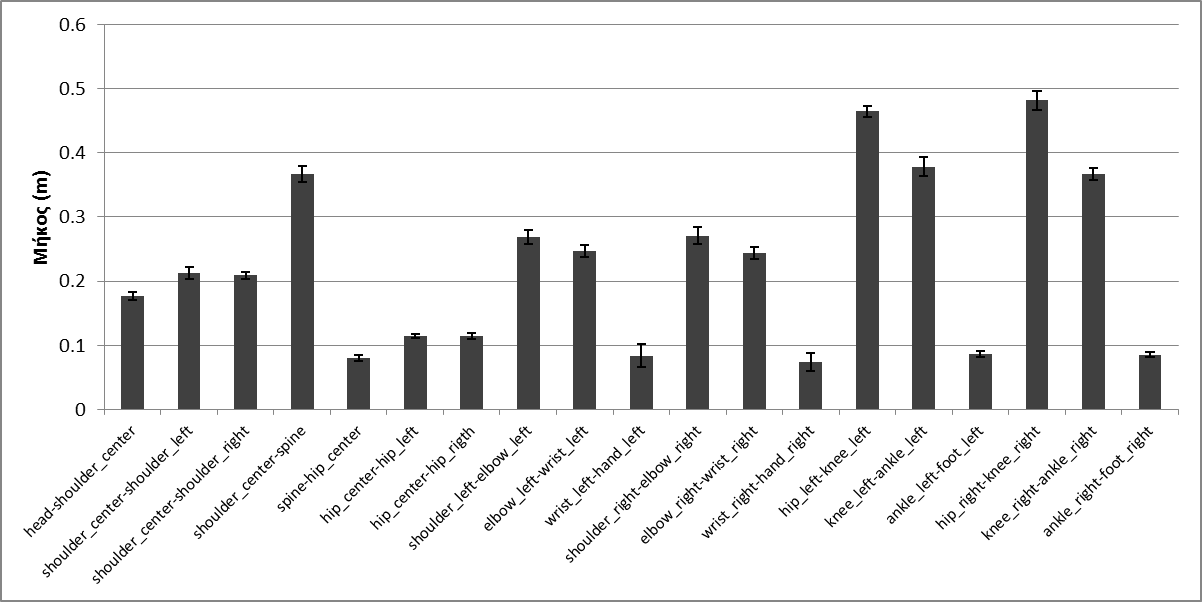
\includegraphics[width=.8\textwidth]{fig/subject01-segments.png}
    \caption{Εκτιμώμενη μέση τιμή σε σύγκριση με την πραγματική τιμή για το μήκος των τμημάτων του σώματος για το πρώτο δείγμα (14 διαφορετικές κινήσεις)}
    \label{fig:subject01-segments}
\end{figure}

Παρατηρούμε ότι οι τυπικές αποκλίσεις είναι μικρές με ελάχιστη για το πρώτο δείγμα στα $std_{min} = 0.003m$ και με μέγιστη τιμή στα $std_{max} = 0.018m$ (Σχήμα \ref{fig:subject01-segments}). Όσον αφορά το δεύτερο δείγμα οι αντίστοιχες τυπικές αποκλίσεις είναι $std_{min} = 0.0002m$, $std_{max} = 0.015m$ αντίστοιχα (Σχήμα \ref{fig:subject02-segments}). Επίσης και για τα δυο δείγματα παρουσιάζονται τα πραγματικά μήκη των τμημάτων του σώματος με σφάλμα μετρήσεων $\pm 1cm$.

\begin{figure}[H]
    \centering
    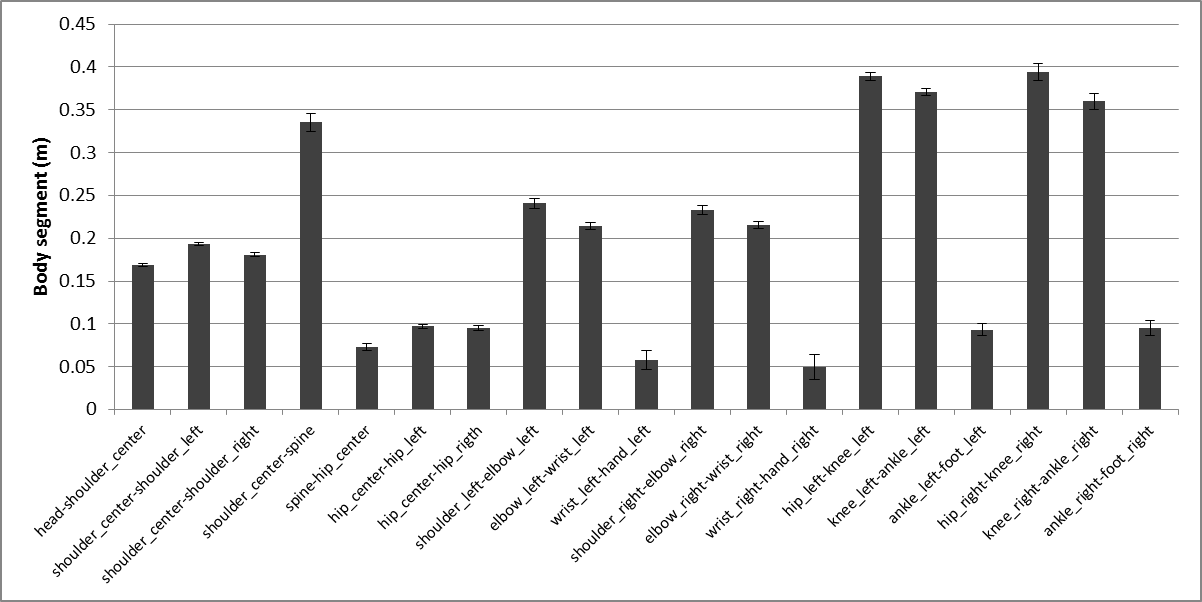
\includegraphics[width=.8\textwidth]{fig/subject02-segments.png}
    \caption{Εκτιμώμενη μέση τιμή σε σύγκριση με την πραγματική τιμή για το μήκος των τμημάτων του σώματος για το δεύτερο δείγμα (5 κινήσεις)}
    \label{fig:subject02-segments}
\end{figure}

\begin{equation}
    \begin{gathered}
        \text{Πρόβλεψη} \\
        \hat{p}_{t} = p_{t-1} + u_{t}, \quad u_{t} = \frac{p_{t-1} - p_{t-2}}{t_{t-1} - t_{t-2}} \\
        \hat{P} = P_{t-1} + Q \\[.5cm]
        \text{Διόρθωση} \\
        Κ = \frac{\hat{P}}{\hat{P} + R}\\
        p_{t} = \hat{p}_{t} + K \cdot (p_{t} - \hat{p}_{t}) \\
        P_{t} = (1 - K) \cdot \hat{P}
    \end{gathered}
    \label{equ:kalman-predict-update}
\end{equation}

Ως δεύτερη σύγκριση του συστήματος, καταγράφτηκε μια κίνηση χωρίς την χρήση κάποιου φίλτρου και στην συνέχεια καταγράφτηκε μια όμοια κίνηση με χρήση φίλτρου και ως παράμετροι επιλέχθηκαν οι τιμές για δυνατό φιλτράρισμα από το Πίνακα \ref{tab:filter-parameters}. Επίσης έγινε μια απλή υλοποίηση ενός φίλτρου \eng{Kalman} με βάση την αναδρομική σχέση \ref{equ:kalman-predict-update} και επιλέχθηκαν τιμές για τα $R = 0.05,\; Q = 0.05$. Στο Σχήμα \ref{fig:no-filter-filter-kalman} στην αριστερή στήλη βρίσκονται οι συντεταγμένες του δεξιού χεριού χωρίς την χρήση κάποιου φίλτρου, ενώ στην δεξιά στήλη με χρήση του δυνατού φίλτρου. Με διακεκομμένες γραμμές φαίνεται η απόκριση του φίλτρου \eng{Kalman}. Στην περίπτωση που επιλέξουμε να χρησιμοποιήσουμε δυνατό φίλτρο δεν διακρίνεται βελτίωση αν χρησιμοποιήσουμε το φίλτρου \eng{Kalman}, όπως έχει υλοποιηθεί. Φαίνεται όμως η ανάγκη για εξομάλυνση, οπότε απλά φίλτρα που φιλτράρουν τις απότομες μεταβολές βελτιώνουν πολύ το αποτέλεσμα.

%\begin{center}
%    \begin{tabular}{cc}
%        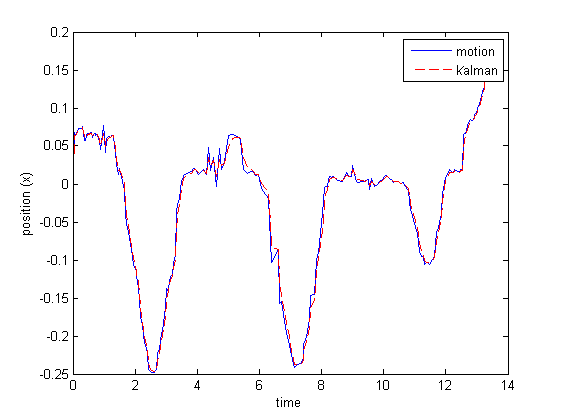
\includegraphics[width=.5\textwidth, height = 0.22\textheight, keepaspectratio]{fig/filter0-x.png} & 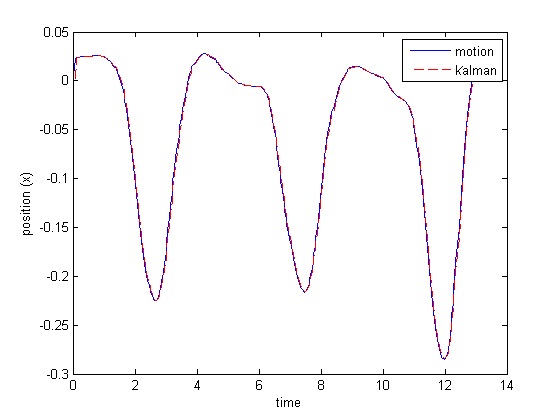
\includegraphics[width=.5\textwidth, height = 0.22\textheight, keepaspectratio]{fig/filter3-x.png}\\
%        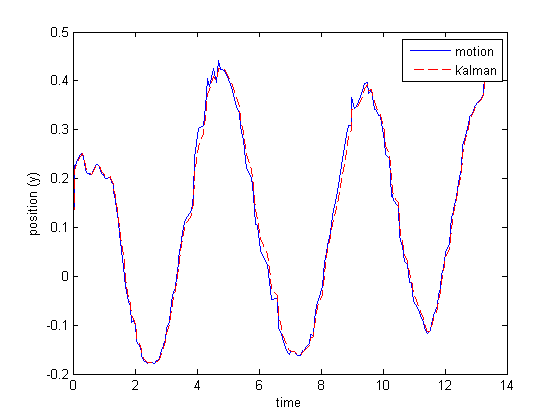
\includegraphics[width=.5\textwidth, height = 0.22\textheight, keepaspectratio]{fig/filter0-y.png} & 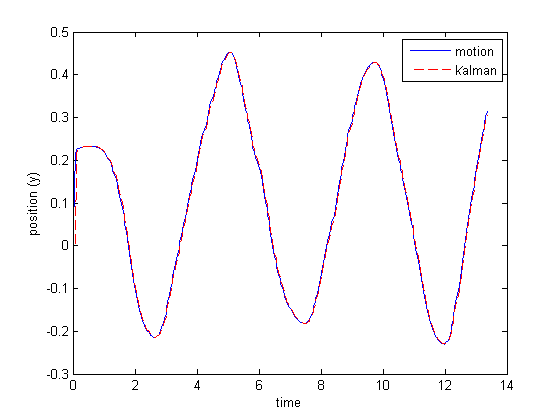
\includegraphics[width=.5\textwidth, height = 0.22\textheight, keepaspectratio]{fig/filter3-y.png}\\
%        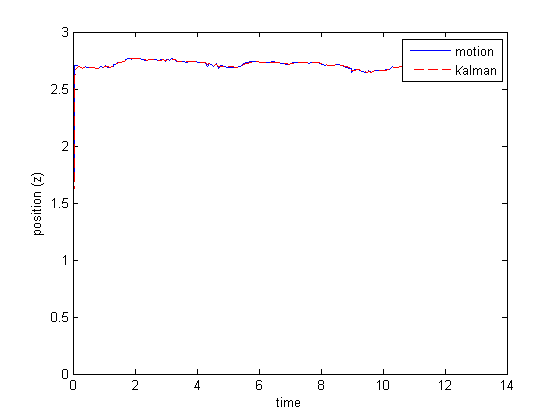
\includegraphics[width=.5\textwidth, height = 0.22\textheight, keepaspectratio]{fig/filter0-z.png} & 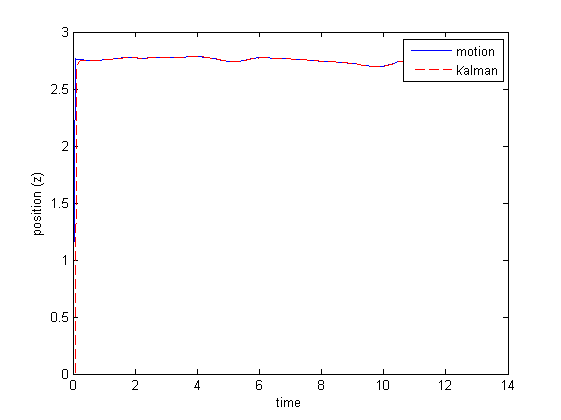
\includegraphics[width=.5\textwidth, height = 0.22\textheight, keepaspectratio]{fig/filter3-z.png}\\
%        \includegraphics[width=.5\textwidth, height = 0.22\textheight, keepaspectratio]{fig/filter0-xyz.png} & \includegraphics[width=.5\textwidth, height = 0.22\textheight, keepaspectratio]{fig/filter3-xyz.png}
%    \end{tabular}
%    \captionof{table}{Συντεταγμένες του δεξιού χεριού στις επιμέρους συνιστώσες (\eng{x, y, z, xyz}) χωρίς φιλτράρισμα (αριστερή στήλη) και με φιλτράρισμα (δεξιά στήλη) με βάση την υλοποίηση μας. Σύγκριση και στις δυο περιπτώσεις με το φίλτρο \eng{Kalman}}
%    \label{tab:no-filter-filter-kalman}
%\end{center}

\begin{figure}[H]
    %\captionsetup[subfigure]{position=b}
    \centering
    \begin{subfigure}[t]{.48\textwidth}
        \includegraphics[width=\textwidth, keepaspectratio]{fig/filter0-x.png}
        \caption{Συντεταγμένη στον \eng{x} άξονα χωρίς φιλτράρισμα}
        \label{fig:filter0-x}
    \end{subfigure}
    \begin{subfigure}[t]{.48\textwidth}
        \includegraphics[width=\textwidth, keepaspectratio]{fig/filter3-x.png}
        \caption{Συντεταγμένη στον \eng{x} άξονα με φιλτράρισμα}
        \label{fig:filter3-x}
    \end{subfigure}

    \centering
    \begin{subfigure}[t]{.48\textwidth}
        \includegraphics[width=\textwidth, keepaspectratio]{fig/filter0-y.png}
        \caption{Συντεταγμένη στον \eng{y} άξονα χωρίς φιλτράρισμα}
        \label{fig:filter0-y}
    \end{subfigure}
    \begin{subfigure}[t]{.48\textwidth}
        \includegraphics[width=\textwidth, keepaspectratio]{fig/filter3-y.png}
        \caption{Συντεταγμένη στον \eng{y} άξονα με φιλτράρισμα}
        \label{fig:filter3-y}
    \end{subfigure}

    \centering
    \begin{subfigure}[t]{.48\textwidth}
        \includegraphics[width=\textwidth, keepaspectratio]{fig/filter0-z.png}
        \caption{Συντεταγμένη στον \eng{z} άξονα χωρίς φιλτράρισμα}
        \label{fig:filter0-z}
    \end{subfigure}
    \begin{subfigure}[t]{.48\textwidth}
        \includegraphics[width=\textwidth, keepaspectratio]{fig/filter3-z.png}
        \caption{Συντεταγμένη στον \eng{z} άξονα με φιλτράρισμα}
        \label{fig:filter3-z}
    \end{subfigure}
    \caption{Συντεταγμένες του δεξιού χεριού στις επιμέρους συνιστώσες (\eng{x, y, z}) χωρίς φιλτράρισμα (αριστερή στήλη) και με φιλτράρισμα (δεξιά στήλη) με βάση την υλοποίηση μας. Σύγκριση και στις δυο περιπτώσεις με το φίλτρο \eng{Kalman}.}
    \label{fig:no-filter-filter-kalman}
\end{figure}

%%%%%%%%%%%%%%%%%%%%%%%%%%%%%%%%%%%%%%%%%%%%%%%%%%%%%%%%%%%%%%%%%%%%%%%%%%%%%%%%
\section{Αντίστροφη Κινηματική}

\begin{figure}[H]
    \centering
    \begin{subfigure}[t]{.48\textwidth}
        \includegraphics[width=\textwidth, keepaspectratio]{fig/ik-reg1.png}
        \caption{Κίνηση μπροστά-πίσω}
        \label{fig:forth-back1}
    \end{subfigure}
    \begin{subfigure}[t]{.48\textwidth}
        \includegraphics[width=\textwidth, keepaspectratio]{fig/ik-reg6.png}
        \caption{Κίνηση μπροστά-πίσω}
        \label{fig:forth-back2}
    \end{subfigure}

    \begin{subfigure}[t]{.48\textwidth}
        \includegraphics[width=\textwidth, keepaspectratio]{fig/ik-reg5.png}
        \caption{Τυχαία κίνηση}
        \label{fig:random-walk1}
    \end{subfigure}
    \begin{subfigure}[t]{.48\textwidth}
        \includegraphics[width=\textwidth, keepaspectratio]{fig/ik-reg4.png}
        \caption{Τυχαία κίνηση}
        \label{fig:random-walk1}
    \end{subfigure}

    \begin{subfigure}[t]{.48\textwidth}
        \includegraphics[width=\textwidth, keepaspectratio]{fig/ik-reg2.png}
        \caption{Κανονική βάδιση}
        \label{fig:noraml-walk}
    \end{subfigure}
    \begin{subfigure}[t]{.48\textwidth}
        \includegraphics[width=\textwidth, keepaspectratio]{fig/ik-reg3.png}
        \caption{Εμπρόσθια προέκταση του ποδιού}
        \label{fig:knee-hip-extension}
    \end{subfigure}
    \caption{Τα τρία είδη σφαλμάτων της αντίστροφης κινηματικής για τις έξι διαφορετικές κινήσεις. Για τα τρία σφάλματα παρουσιάζονται η μέγιστη τιμή, η μέση τιμή και η τυπική απόκλιση που υπολογίστηκε με βάση την χρονοσειρά των σφαλμάτων.}
    \label{fig:ik-error-regions}
\end{figure}

Για να υπάρξουν σωστά αποτελέσματα κατά την αντίστροφη κινηματική είναι αναγκαία η διαδικασία της κανονικοποίησης, ώστε το γενικό μοντέλο να πάρει τις διαστάσεις του δείγματος, οπότε η διαδικασία της κανονικοποίησης θεωρείται δεδομένη κάθε φορά. Αυτό που μπορούμε να εκθέσουμε ως αποτέλεσμα της διαδικασίας είναι τα σφάλματα της αντίστροφης κινηματικής. Για το πείραμα εκτελέστηκε η αντίστροφη κινηματική για 6 διαφορετικές κινήσεις (Σχήμα \ref{fig:ik-error-regions}) του ίδιου δείγματος και καταγράφηκε το συνολικό αθροιστικό σφάλμα (\eng{total RMS error}), το σφάλμα λόγω ενδείξεων (\eng{marker error}) και το μέγιστο σφάλμα από όλες τις αρθρώσεις (\eng{max joint error}). Το συνολικό αθροιστικό σφάλμα λαμβάνεται ως το σφάλμα που οφείλεται στην διαφορά των συντεταγμένων του μοντέλου και της πειραματικής κίνησης. Το σφάλμα λόγω ενδείξεων υπολογίζεται με βάση την Ευκλείδεια απόσταση των ενδείξεων του μοντέλου και των αντίστοιχων πειραματικών. Όσον αφορά το μέγιστο σφάλμα άρθρωσης αφορά την άρθρωση που συνεισφέρει περισσότερο στο σφάλμα. Τα τρία αυτά σφάλματα ήταν διαθέσιμα για κάθε χρονική στιγμή που υπολογίζονταν η αντίστροφη κινηματική. Ως εκ τούτο για κάθε ένα από αυτά τα σφάλματα υπολογίστηκε η μέση τιμή, η τυπική απόκλιση και η μέγιστη τιμή από όλες τις χρονικές στιγμές για κάθε κίνηση ξεχωριστά. Με βάση την βιβλιογραφία αναφέρεται ότι το συνολικό αθροιστικό σφάλμα πρέπει να είναι μικρότερο του $0.01cm$ και για το σφάλμα λόγω ενδείξεων να κυμαίνεται στα όρια $[0.02-0.04cm]$, ώστε να έχουμε ικανοποιητική ανοχή στα αποτέλεσμα της αντίστροφης κινηματικής. Και για τα δυο σφάλματα ήμαστε αρκετά εντός του ορίου.

%\begin{center}
%    \begin{tabular}{cc}
%        \includegraphics[width=.48\textwidth, keepaspectratio]{fig/ik-reg1.png} & \includegraphics[width=.48\textwidth, keepaspectratio]{fig/ik-reg2.png}\\[3pt]
%        \includegraphics[width=.48\textwidth, keepaspectratio]{fig/ik-reg3.png} & \includegraphics[width=.48\textwidth, keepaspectratio]{fig/ik-reg4.png}\\[3pt]
%        \includegraphics[width=.48\textwidth, keepaspectratio]{fig/ik-reg5.png} & \includegraphics[width=.48\textwidth, keepaspectratio]{fig/ik-reg6.png}
%    \end{tabular}
%    \captionof{table}{Τα τρία είδη σφαλμάτων της αντίστροφης κινηματικής για τις έξι διαφορετικές κινήσεις. Για τα τρία σφάλματα παρουσιάζονται η μέγιστη τιμή, η μέση τιμή και η τυπική απόκλιση που υπολογίστηκε με βάση την χρονοσειρά των σφαλμάτων.}
%    \label{tab:ik-error-regions}
%\end{center}

\begin{figure}[H]
    \centering
    \includegraphics[width=0.8\textwidth, keepaspectratio]{fig/ik-no-scale-with-scale.png}
    \caption{Σύγκριση της βελτίωσης των σφαλμάτων της αντίστροφης κινηματικής με ή χωρίς την εκτέλεση της κανονικοποίησης}
    \label{fig:ik-no-scale-with-scale}
\end{figure}

Στο Σχήμα \ref{fig:ik-no-scale-with-scale} έγινε σύγκριση της αποτελεσματικότητας της διαδικασία κανονικοποίησης στο αποτέλεσμα της αντίστροφης κινηματικής. Η πρώτη τριάδα των μετρήσεων αφορά τα σφάλματα της αντίστροφης κινηματικής χωρίς την διεξαγωγή κανονικοποίησης, ενώ η δεύτερη τριάδα με διεξαγωγή της κανονικοποίησης. Παρατηρείται μεγάλη βελτίωση των σφαλμάτων και ιδιαίτερα στα σφάλματα μέσης τιμής. Ωστόσο δεν παρατηρείται σημαντική βελτίωση στα σφάλματα της μέγιστης τιμής σφάλματος της άρθρωσης. Δηλαδή υπάρχουν κάποιες αρθρώσεις που δίνουν μεγάλο σφάλμα, αλλά γενικά έχουμε βελτίωση ως προς το μέσο όρο των αρθρώσεων.

%%%%%%%%%%%%%%%%%%%%%%%%%%%%%%%%%%%%%%%%%%%%%%%%%%%%%%%%%%%%%%%%%%%%%%%%%%%%%%%%
\section{Αντίστροφη Δυναμική}

\begin{figure}[H]
    \centering
    \begin{subfigure}[t]{.48\textwidth}
        \includegraphics[width=\textwidth, keepaspectratio]{fig/id-hip.png}
        \caption{Ροπή στο γοφό για έναν κύκλο βάδισης (πειραματικά)}
        \label{fig:hip-moment}
    \end{subfigure}
    \begin{subfigure}[t]{.48\textwidth}
        \includegraphics[width=\textwidth, keepaspectratio]{fig/id-hip-ref.png}
        \caption{Ροπή του γοφό για έναν κύκλο βάδισης (βιβλιογραφία)}
        \label{fig:hip-moment-ref}
    \end{subfigure}

    \centering
    \begin{subfigure}[t]{.48\textwidth}
        \includegraphics[width=\textwidth, keepaspectratio]{fig/id-knee.png}
        \caption{Ροπή στο γόνατο για έναν κύκλο βάδισης (πειραματικά)}
        \label{fig:knee-moment}
    \end{subfigure}
    \begin{subfigure}[t]{.48\textwidth}
        \includegraphics[width=\textwidth, keepaspectratio]{fig/id-knee-ref.png}
        \caption{Ροπή στο γονάτο για έναν κύκλο βάδισης (βιβλιογραφία)}
        \label{fig:knee-moment-ref}
    \end{subfigure}

    \centering
    \begin{subfigure}[t]{.48\textwidth}
        \includegraphics[width=\textwidth, keepaspectratio]{fig/id-ankle.png}
        \caption{Ροπή στο αστράγαλο για έναν κύκλο βάδισης (πειραματικά)}
        \label{fig:ankle-moment}
    \end{subfigure}
    \begin{subfigure}[t]{.48\textwidth}
        \includegraphics[width=\textwidth, keepaspectratio]{fig/id-ankle-ref.png}
        \caption{Ροπή στον αστράγαλο για έναν κύκλο βάδισης (βιβλιογραφία)}
        \label{fig:ankle-moment-ref}
    \end{subfigure}
    \caption{Σύγκριση εκτιμώμενων ροπών και των αντίστοιχων ροπών με βάση την βιβλιογραφία \cite{whittlesey} για ένα κύκλο βάδισης}
    \label{fig:id-hip-knee-ankle-moments}
\end{figure}

Με την αντίστροφη δυναμική έχουμε στην διάθεση μας τις ροπές που ασκούνται στις αρθρώσεις κάθε χρονική στιγμή. Λόγω της δυσκολίας υπολογισμού των εξωτερικών δυνάμεων, χρησιμοποιήθηκαν δεδομένα βάδισης και καταγεγραμμένη αντίδραση εδάφους που βρέθηκε στο διαδίκτυο, ώστε να επιβεβαιωθεί η ισχύς της ανάλυσης, αλλά και την ακρίβεια του μοντέλου που μελετάμε. Στην μελέτη των δυνάμεων, παρουσιάζονται οι ροπές του γοφού, του γονάτου και του αστράγαλου για ένα κύκλο βάδισης και συγκρίνονται με την βιβλιογραφία \cite{whittlesey}. Στο Σχήμα \ref{fig:id-hip-knee-ankle-moments} αριστερά βρίσκονται οι πειραματικές ροπές για έναν κύκλο βάδισης και δεξιά τα αντίστοιχα με βάση τη βιβλιογραφία. Τα αποτελέσματα συμβαδίζουν με εκείνα της βιβλιογραφίας αν λάβουμε υπόψιν τις ενδείξεις πάνω στα διαγράμματα. Επίσης παρατηρείται απόκλιση στις μέγιστες και ελάχιστες τιμές με εκείνες τις βιβλιογραφίας, επειδή για τα αποτελέσματα της βιβλιογραφίας χρησιμοποιείται το μοντέλο όλου του σώματος, ενώ στα δικά μας χρησιμοποιείται μόνο το κάτω μέρος του σώματος με αποτέλεσμα να ζυγίζει λιγότερο και η απαιτούμενη ροπή στις αρθρώσεις να είναι μικρότερη. Ωστόσο ποιοτικά τα αποτελέσματα μας συμβαδίζουν με τα προβλεπόμενα.

%\begin{center}
%    \begin{tabular}{cc}
%        \includegraphics[width=.48\textwidth, keepaspectratio]{fig/id-hip.png} & \includegraphics[width=.48\textwidth, keepaspectratio]{fig/id-hip-ref.png}\\[3pt]
%        \includegraphics[width=.48\textwidth, keepaspectratio]{fig/id-knee.png} & \includegraphics[width=.48\textwidth, keepaspectratio]{fig/id-knee-ref.png}\\[3pt]
%        \includegraphics[width=.48\textwidth, keepaspectratio]{fig/id-ankle.png} & \includegraphics[width=.48\textwidth, keepaspectratio]{fig/id-ankle-ref.png}
%    \end{tabular}
%    \captionof{table}{Σύγκριση εκτιμώμενων ροπών και των αντίστοιχων ροπών με βάση την βιβλιογραφία \cite{whittlesey} για ένα κύκλο βάδισης.}
%    \label{tab:id-hip-knee-ankle-moments}
%\end{center}

%%%%%%%%%%%%%%%%%%%%%%%%%%%%%%%%%%%%%%%%%%%%%%%%%%%%%%%%%%%%%%%%%%%%%%%%%%%%%%%%
\section{Μυϊκή Συσχέτιση}

Στο παρακάτω Σχήμα \ref{fig:iber-length-vs-knee-angle} φαίνεται η μεταβολή του μήκους των δυο μυών συναρτήσει την αλλαγή της γωνίας της άρθρωσης δράσεως. Οι δύο μύες ο \eng{rectus femoris} και \eng{vastus intermedius} δρουν στο γόνατο ως καμπτήρες. Ο \eng{rectus femoris} είναι ένας μυς που ξεκινά από την λεκάνη και καταλήγει στην επιγονατίδα, ενώ  ο \eng{vastus intermedius} ξεκινά από την μέση του μηρού και καταλήγει πάλι στην επιγονατίδα. Είναι προφανές ότι όταν το πόδι είναι τεντωμένο τα μήκη των δύο μυών είναι ελάχιστα, ενώ όταν το γόνατο λυγίζει τότε μεγαλώνει το μήκος τους.

\begin{figure}[H]
    \centering
    \includegraphics[width=0.8\linewidth, keepaspectratio]{fig/fiber-length-vs-knee-angle.png}
    \caption{Μήκη των δυο μυών του τετρακέφαλου συναρτήσει της γωνίας της άρθρωσης του γονάτου}
    \label{fig:iber-length-vs-knee-angle}
\end{figure}

Στο δεύτερο Σχήμα \ref{fig:moment-arm-vs-knee-angle} γίνεται μια γεωμετρική ερμηνεία που σχετίζεται με την τοποθέτηση των μυών. Η παράμετρος είναι η ποσότητα που μετατρέπει την δύναμη που παράγει ο μυς σε ροπή στην άρθρωση, η λεγόμενη \eng{muscle moment arm}, για την οποία έγινε συζήτηση στην Παράγραφο \ref{subsec:muscle}. Το σημείο ασυνέχειας ($-85^{\circ}$) που παρατηρείται, οφείλεται στο γεγονός ότι για την συγκεκριμένη γωνία οι μύες ξεκινούν να τυλίγονται γύρω από την επιγονατίδα και το μήκος τους διαμερίζεται κατάλληλα με αποτέλεσμα να υπάρχουν ασυνέχειες στους υπολογισμούς.

\begin{figure}[H]
    \centering
    \includegraphics[width=0.8\linewidth, keepaspectratio]{fig/moment-arm-vs-knee-angle.png}
    \caption{Η ποσότητα \eng{moment arm} των δυο μυών του τετρακέφαλου συναρτήσει της γωνίας της άρθρωσης του γονάτου}
    \label{fig:moment-arm-vs-knee-angle}
\end{figure}

Μια άλλη σημαντική ποσότητα είναι η παραγόμενη δύναμη του μυ συναρτήσει της γενικευμένης συντεταγμένης στην άρθρωση. Παρόλο που η μυϊκή δύναμη εξαρτάται από πολλούς παράγοντες μπορεί να γίνει μια ποιοτική αναπαράσταση την κυματομορφής της. Με βάση την θεωρία (Παράγραφος \ref{subsec:muscle-model}) ο μυς έχει ένα παθητικό μέρος που παράγει μια δύναμη όταν αυτός επιμηκύνεται πάνω από ένα όριο και έναν συσταλτικό μηχανισμό που παράγει την δύναμη του μυ, όπου η κυματομορφή της δύναμης έχει κωδωνοειδείς μορφή. Όπως φαίνεται στο Σχήμα \ref{fig:total-fiber-force}, όπου βλέπουμε το άθροισμα των δυο δυνάμεων, για $-60^{\circ}$ ξεκινά να επιδρά η παθητική δύναμη όσο μικρύνει η γωνία, ενώ για διάστημα $[-60^{\circ},\quad 0^{\circ}]$ έχουμε την κωδωνοειδείς μορφή της ενεργητικής δύναμης του μυ.

\begin{figure}[H]
    \centering
    \includegraphics[width=0.8\linewidth, keepaspectratio]{fig/total-fiber-force.png}
    \caption{Η συνολική δύναμη των δυο μυών του τετρακέφαλου συναρτήσει της γωνίας της άρθρωσης του γονάτου}
    \label{fig:total-fiber-force}
\end{figure}

%%%%%%%%%%%%%%%%%%%%%%%%%%%%%%%%%%%%%%%%%%%%%%%%%%%%%%%%%%%%%%%%%%%%%%%%%%%%%%%%
\section{Εκτέλεση Ορθής Δυναμικής}

\begin{figure}[H]
    \centering
    \begin{subfigure}[t]{.48\textwidth}
        \includegraphics[width=\textwidth, keepaspectratio]{fig/hip-ik-cmc.png}
        \caption{Συντεταγμένη του γοφού}
        \label{fig:hip-cmc}
    \end{subfigure}
    \begin{subfigure}[t]{.48\textwidth}
        \includegraphics[width=\textwidth, keepaspectratio]{fig/knee-ik-cmc.png}
        \caption{Συντεταγμένη του γονάτου}
        \label{fig:knee-cmc}
    \end{subfigure}

    \centering
    \begin{subfigure}[t]{.48\textwidth}
        \includegraphics[width=\textwidth, keepaspectratio]{fig/hip-ik-cmc-na.png}
        \caption{Συντεταγμένη του γοφού}
        \label{fig:hip-cmc-na}
    \end{subfigure}
    \begin{subfigure}[t]{.48\textwidth}
        \includegraphics[width=\textwidth, keepaspectratio]{fig/ankle-ik-cmc-na.png}
        \caption{Συντεταγμένη του γονάτου}
        \label{fig:knee-cmc-na}
    \end{subfigure}

    \centering
    \begin{subfigure}[t]{.48\textwidth}
        \includegraphics[width=\textwidth, keepaspectratio]{fig/hip-ik-id.png}
        \caption{Συντεταγμένη του γοφού}
        \label{fig:hip-id}
    \end{subfigure}
    \begin{subfigure}[t]{.48\textwidth}
        \includegraphics[width=\textwidth, keepaspectratio]{fig/knee-ik-id.png}
        \caption{Συντεταγμένη του γονάτου}
        \label{fig:knee-id}
    \end{subfigure}
    \caption{Σύγκριση της ευστάθειας της ορθής δυναμικής για δυο αρθρώσεις (γοφός, γόνατο). Τροφοδοτούμε την ορθή δυναμική με το αποτέλεσμα της διαδικασία υπολογισμού μυϊκών διεγέρσεων με χρήση εφεδρικών κινητήρων στις αρθρώσεις \ref{fig:hip-cmc}, \ref{fig:knee-cmc}, το ίδιο αλλά χωρίς εφεδρικούς κινητήρες \ref{fig:hip-cmc-na}, \ref{fig:knee-cmc-na} και τέλος συγκρίνουμε με το αν χρησιμοποιήσουμε το αποτέλεσμα της αντίστροφης δυναμικής \ref{fig:hip-id}, \ref{fig:knee-id}.}
    \label{fig:fd-cmc-id}
\end{figure}

Σε αυτή την παράγραφο θα αναφερθούμε για την ευστάθεια που επιτυγχάνεται ανάλογα με την κατηγορία μεθόδων που χρησιμοποιούνται. Η ευστάθεια ανταποκρίνεται στη συσσώρευση σφαλμάτων στα στάδια μέχρι τον υπολογισμό των διεγέρσεων, που μπορεί να είναι είτε ροπές, είτε νευρικές διεγέρσεις. Στο πρώτο πείραμα μετά την αντίστροφη κινηματική εκτελούμε την διαδικασία του υπολογισμού των μυϊκών διεγέρσεων (Σχήμα \ref{fig:hip-cmc-na}, Σχήμα \ref{fig:knee-cmc-na}), όπου υπολογίζουμε τις διεγέρσεις των μυών που απαιτούνται για την παραγωγή της καταγεγραμμένης κίνησης και κατόπιν εκτελούμε ορθή δυναμική. Πρέπει να αναφέρουμε ότι κατά την διεξαγωγή των πειραμάτων εισάγονται εφεδρικοί κινητήρες (Σχήμα \ref{fig:hip-cmc}, Σχήμα \ref{fig:knee-cmc}), οι οποίοι είναι σε θέση να τροφοδοτήσουν επιπλέον ροπή στις αρθρώσεις όταν οι μύες δεν την διαθέτουν. Για το λόγο αυτό στα αποτελέσματα γίνεται σύγκριση μεταξύ χρήση ή μη των εφεδρικών κινητήρων. Στο δεύτερο πείραμα μετά την αντίστροφη κινηματική εκτελούμε αντίστροφη δυναμική και τροφοδοτούμε στη συνέχεια τις υπολογισμένες ροπές στην διαδικασία της ορθής δυναμικής ώστε να γίνει σύγκριση (Σχήμα \ref{fig:hip-id}, Σχήμα \ref{fig:knee-id}). Στο Σχήμα \ref{fig:fd-cmc-id} εξετάζονται οι γενικευμένες συντεταγμένες για τον γοφό και το γόνατο. Με κόκκινο είναι η επιθυμητή τροχιά με βάση το αποτέλεσμα της αντίστροφης κινηματικής ενώ με μπλε το αποτέλεσμα των γενικευμένων συντεταγμένων από την ορθή δυναμική. Παρατηρούμε τη μεγάλη σύγκλιση που επιτυγχάνεται με χρήση της μεθόδου υπολογισμού των μυϊκών διεγέρσεων σε συνδυασμό με χρήση εφεδρικών κινητήρων σε σχέση με την αντίστροφη δυναμική. Ωστόσο μετά από κάποια χρονική στιγμή η προτεινόμενη μέθοδος μπαίνει και αυτή στην αστάθεια, γεγονός επίσης αναμενόμενο.

%\begin{center}
%    \begin{tabular}{cc}
%        \includegraphics[width=.48\textwidth, keepaspectratio]{fig/hip-ik-cmc.png} & \includegraphics[width=.48\textwidth, keepaspectratio]{fig/knee-ik-cmc.png}\\[3pt]
%        \includegraphics[width=.48\textwidth, keepaspectratio]{fig/hip-ik-cmc-na.png} & \includegraphics[width=.48\textwidth, keepaspectratio]{fig/ankle-ik-cmc-na.png}\\[3pt]
%        \includegraphics[width=.48\textwidth, keepaspectratio]{fig/hip-ik-id.png} & \includegraphics[width=.48\textwidth, keepaspectratio]{fig/knee-ik-id.png}
%    \end{tabular}
%    \captionof{table}{Σύγκριση της ευστάθειας της ορθής δυναμικής}
%    \label{tab:fd-cmc-id}
%\end{center}

Στο Σχήμα \ref{fig:rf-vasint-activation} παρουσιάζεται το αποτέλεσμα των νευρικών διεγέρσεων για τους δυο μύες \eng{rectus femoris} και \eng{vastus intermedius}. Η επιβεβαίωση μπορεί να γίνει ποιοτικά με μετρήσεις από τα \eng{EMG}, ωστόσο δεν τις έχουμε στην διάθεση μας.

\begin{figure}[H]
    \centering
    \includegraphics[width=0.8\linewidth, keepaspectratio]{fig/rf-vasint-activation.png}
    \caption{Μυϊκή ενεργοποίηση για τους δυο μύες του τετρακέφαλου}
    \label{fig:rf-vasint-activation}
\end{figure}

%\vfill
%%%%%%%%%%%%%%%%%%%%%%%%%%%%%%%%%%%%%%%%%%%%%%%%%%%%%%%%%%%%%%%%%%%%%%%%%%%%%%%%
\section{Εφαρμογές και Μελλοντική Επέκταση της Εργασίας}

Αρχικά θα αναφερθούμε σε συγκεκριμένα σημεία της παρούσας εργασίας που απαιτούν βελτίωση και είναι ενεργό πεδίο έρευνας, ενώ στην συνέχεια θα γίνει μια συζήτηση για πιθανά ενδιαφέρουσες εφαρμογές. Κατά τα στάδια της ανάλυσης έγιναν πολλές προσεγγίσεις που οδηγούν σε εσφαλμένη εκτίμηση της δυναμικής συμπεριφοράς του δείγματος κατά την διεξαγωγή των κινήσεων.

Ξεκινώντας από το στάδιο της καταγραφής της κίνησης, η υλοποίηση που δώσαμε, πάσχει από αρκετά προβλήματα που είναι αναπόφευκτα. Ενδεικτικά δυο σημεία που θα μπορούσαν να βελτιώσουν κατά πολύ το αποτέλεσμα είναι η αντιμετώπιση της παρεμπόδισης και η προσπάθεια καταγραφής πολλαπλών σημείων του σώματος πέραν των αρθρώσεων. Το πρώτο μπορεί να λυθεί αν χρησιμοποιηθούν πολλαπλές συσκευές καταγραφής τοποθετημένες σε διαφορετικές οπτικές γωνίες σε σχέση με το δείγμα. Όσον αφορά το δεύτερο πρόβλημα θα μπορούσε να υλοποιηθεί κατάλληλος αλγόριθμος καταγραφής της κίνησης ο οποίος θα ανιχνεύει περισσότερα σημεία πάνω στο σώμα, με αποτέλεσμα να μπορούμε να έχουμε μοναδική λύση στο πρόβλημα της θέσης και του προσανατολισμού των τμημάτων του σώματος. Επαγγελματικά συστήματα καταγραφής ασχολούνται με το πως θα εκτιμήσουν την θέση των ενδείξεων λαμβάνοντας υπόψιν και την κίνηση του δέρματος. Συμπερασματικά, αντιλαμβανόμαστε την πολυπλοκότητα του προβλήματος αλλά και την απαίτηση για τη μείωση του σφάλματος της καταγεγραμμένης κίνησης.

Όσον αφορά το μοντέλο που χρησιμοποιήθηκε έχουν γίνει πολλές προσεγγίσεις. Είναι γνωστό ότι κάθε άνθρωπος έχει τις ιδιαιτερότητες του, τόσο στην δυνατότητα κίνησης, όσο και στην γεωμετρική διάταξη του σκελετού, αλλά και στην γεωμετρική τοποθέτηση των μυών. Έχουμε εισάγει τρομερές προσεγγίσεις στους βαθμούς ελευθερίας της διάταξής, οι οποίες δεν αντιπροσωπεύουν αποτελεσματικά την πραγματική κίνησης των ανθρώπινων τμημάτων. Για παράδειγμα το γόνατο πέραν της περιστροφικής του ικανότητας εκτελεί και μετατοπίσεις, κάτι που δεν λάβαμε. Τα τελευταία χρόνια γίνεται μια προσπάθεια σάρωσης του δείγματος πριν το πείραμα, χρησιμοποιώντας μαγνητικό τομογράφο και άλλες συσκευές, συνεπώς με βάση το αποτέλεσμα τους δημιουργείται ένα μοντέλο του σκελετού αλλά και της μυϊκής διάταξης. Όσον αφορά τους μύες με βάση το τελευταίο γίνεται μια προσπάθεια, έτσι ώστε ο μυς να μην θεωρείται ένα ευθύγραμμο τμήμα, αλλά να έχει το δικό του όγκο και να αλληλεπιδρά με το γύρω περιβάλλον του. Ωστόσο όλες αυτές οι βελτιώσεις αυξάνουν την πολυπλοκότητα του μοντέλου.

Ενδιαφέρουσα εφαρμογή θα ήταν η συλλογή αποτελεσμάτων που θα μπορούσαν να βοηθήσουν τους ερευνητές, ώστε να κατανοήσουν τα αίτια των ασθενειών με βάση του εικονικού μοντέλου, δίνοντας αποτελέσματα που δεν είναι εύκολα μετρήσιμα. Ακόμη οι τεχνικές που αναπτύχθηκαν στα πλαίσια της παρούσας διπλωματικής εργασίας να εφαρμοστούν στην πράξη και να είναι ένα καθημερινό εργαλείο-ρουτίνα στην εξέταση του ασθενή. Επίσης μπορούν να αναπτυχθούν λύσεις οι οποίες θα παρέχουν την εξέταση μια δυσλειτουργίας ακόμη και από το σπίτι, αλλά και να ενημερώνεται ο υπεύθυνος ιατρό ηλεκτρονικά για την κατάσταση του ασθενή. Όπως αναφέρθηκε και στην εισαγωγή ενδιαφέρον παρουσιάζει και η εφαρμογή τεχνικών προσομοίωσης κατά την παρασκευή φαρμάκων για την θεραπεία του ασθενή.

Τέλος, κάτι που ανήκει σε διαφορετικό κλάδο από την ιατρική είναι η δημιουργία ενός εικονικού προφίλ του δείγματος με βάση την φυσιολογία του κατά την διεξαγωγή κάποιας κίνησης και η εκτίμηση των παραμέτρων που συμβάλουν σε αυτήν. Ως εκ τούτου ανοίγεται ένας μεγάλος ορίζοντας εφαρμογών που μπορούν να βασιστούν στις εικονικές παραμέτρους. Ένα παράδειγμα είναι η ρεαλιστική αναπαράσταση του ανθρώπινου σώματος κατά την διεξαγωγή κάποιας δραστηριότητας που θα μπορούσε να αναπαραστήσει ακόμα και τις νευρικές απολήξεις, ωστόσο απαιτείται βαθιά γνώση και μοντελοποίηση του ανθρώπινου σώματος. Επίσης είναι εφικτή η σύνθεση διαφορετικών δραστηριοτήτων με χρήση μόνο μιας καταγεγραμμένης κίνησης η οποία θα φέρει τα χαρακτηριστικά του δείγματος, καθιστώντας το χρήσιμο εργαλείο για τους \eng{animators}.

%%%%%%%%%%%%%%%%%%%%%%%%%%%%%%%%%%%%%%%%%%%%%%%%%%%%%%%%%%%%%%%%%%%%%%%%%%%%%%%%
\section{Συμπεράσματα}

Στην παρούσα εργασία δείξαμε τη δυνατότητα καταγραφής της ανθρώπινης κίνησης με μια φθηνή συσκευή (συγκριτικά με άλλα συστήματα καταγραφής) όπως είναι το \eng{Kinect} για την επίτευξη αξιόλογων αποτελεσμάτων με ελάχιστο κόπο από την πλευρά του προγραμματιστή. Επιπλέον δείξαμε πώς με απλές μεθόδους φιλτραρίσματος μπορεί να βελτιωθεί κατά πολύ το αποτέλεσμα της καταγεγραμμένης κίνησης, ώστε να είναι κατάλληλο για επεξεργασία στα μετέπειτα στάδια. Επίσης κατέστη σαφής η δυνατότητα του \eng{Kinect} να προσδιορίζει τα μορφομετρικά χαρακτηριστικά του ανθρώπου με μεγάλη ακρίβεια.

Στην συνέχεια αποδείξαμε ότι μαζί με την καταγεγραμμένη κίνηση και ένα αξιόπιστο μοντέλο μπορούν να γίνουν πολλές και διάφορες αναλύσεις, που είναι σε θέση να βοηθήσουν τους αναλυτές να εξάγουν συμπεράσματα για το δείγμα. Ως εκ τούτου, απαραίτητο στάδιο της ανάλυσης είναι η αντίστροφη κινηματική, ενώ η μείωση των σφαλμάτων είναι κομβικό σημείο στην ανάλυση. Τονίσαμε την σημασία της αντίστροφης δυναμικής ως εργαλείο ανάλυσης και παρουσιάσαμε τα αποτελέσματα της βάδισης τα οποία συμφωνούν με τη βιβλιογραφία. Παρουσιάσαμε τα αποτέλεσμα της μεθοδολογίας παραγωγής μεγαλύτερης διάρκειας ευσταθούς βάδισης που συμβάδιζαν με μικρή απόκλιση από την επιθυμητή κίνηση. Στα πλαίσια των αναλύσεων μπορούν να εξαχθούν και άλλα αποτελέσματα, όπως είναι οι νευρικές διεγέρσεις, οι δυνάμεις που ασκούν οι μύες, τα μήκη τους κατά την βάδιση και δυνάμεις αντίδρασης μεταξύ των οστών, ωστόσο η πειραματική τους επιβεβαίωση είναι δύσκολη στην πράξη.

Κατά την περιγραφή των μεθόδων ανάλυσης έγιναν συγκρίσεις και αναφέρθηκαν τα μειονεκτήματα και τα πλεονεκτήματα τους. Κατά την σχεδίαση του μοντέλου έγιναν κάποιες παραδοχές που αφορούσαν στην κινητικότητα του, την γεωμετρική τοποθέτηση των μυών και την κατανομή της μάζας. Όλα αυτά οδηγούν σε σφάλματα στις εκτιμώμενες ποσότητες και ανάλογα με τις ανοχές που έχουμε θέσει με βάση το πρόβλημα ίσως απαιτείται εναλλακτική προσέγγιση. Ωστόσο οι προσεγγίσεις που υιοθετήσαμε οδηγούν σε ορθά αποτελέσματα με μικρές αποκλίσεις από την πραγματικότητα.

Υπάρχει μεγάλο περιθώριο βελτίωσης για την εφεύρεση νέων, πιο γρήγορων, πιο ακριβών μεθόδων. Ειδικά το θέμα του χρόνου που απαιτούν κάποιες αναλύσεις είναι απαγορευτικό πολλές φορές, αλλά και αναπόφευκτο για ένα τόσο δύσκολο πρόβλημα. Η πρόοδος των μεθόδων προσομοίωσης σε συνδυασμό με συστήματα καταγραφής και μεθόδους ανάλυσης μπορούν να χρησιμοποιηθούν στην ιατρική και σε άλλους κλάδους και να γίνουν δεδομένα εργαλεία στην καθημερινότητα, βελτιώνοντας την ποιότητα των υπηρεσιών.


\bibliographystyle{acm}
\bibliography{bibliography/bibliography}

\end{document} 